%  ========================================================================
%  Copyright (c) 1985-2014 The University of Washington
%
%  Licensed under the Apache License, Version 2.0 (the "License");
%  you may not use this file except in compliance with the License.
%  You may obtain a copy of the License at
%
%      http://www.apache.org/licenses/LICENSE-2.0
%
%  Unless required by applicable law or agreed to in writing, software
%  distributed under the License is distributed on an "AS IS" BASIS,
%  WITHOUT WARRANTIES OR CONDITIONS OF ANY KIND, either express or implied.
%  See the License for the specific language governing permissions and
%  limitations under the License.
%  ========================================================================
%

% Documentation for University of Washington thesis LaTeX document class
% by Jim Fox
% fox@washington.edu
%
%    Revised for version 2015/03/03 of uwthesis.cls
%
%    This document is contained in a single file ONLY because
%    I wanted to be able to distribute it easily.  A real thesis ought
%    to be contained on many files (e.g., one for each chapter, at least).
%
%    To help you identify the files and sections in this large file
%    I use the string '==========' to identify new files.
%
%    To help you ignore the unusual things I do with this sample document
%    I try to use the notation
%
%    % --- sample stuff only -----
%    special stuff for my document, but you don't need it in your thesis
%    % --- end-of-sample-stuff ---


%    Printed in twoside style now that that's allowed
%

\documentclass [11pt, proquest] {uwthesis}[2015/03/03]

% The following line would print the thesis in a postscript font
\usepackage{natbib}
\usepackage{bibentry}
\nobibliography*
\def\bibpreamble{\protect\addcontentsline{toc}{chapter}{Bibliography}}

\setcounter{tocdepth}{1}  % Print the chapter and sections to the toc


% ==========   Local defs and mods
\usepackage{mdframed} % box for science questions
\usepackage{textcomp} % copyright symbol
\usepackage{amsmath} % equations on ch4
\usepackage[final]{graphicx} % graphics
\usepackage{hanging} % hanging bib entry
\DeclareGraphicsExtensions{.pdf, .png, .jpg, .eps}
\graphicspath{{./figs/ch1/}{./figs/ch2/}{./figs/ch3/}{./figs/ch4/}{./figs/ch5/}}
\newcommand\hangbibentry[1]{%
    \smallskip\par\hangpara{1em}{1}\bibentry{#1}.\smallskip\par %{indent}{afterline}
}
% --- sample stuff only -----
% These format the sample code in this document

\usepackage{alltt}  %
\newenvironment{demo}
  {\begin{alltt}\leftskip3em
     \def\\{\ttfamily\char`\\}%
     \def\{{\ttfamily\char`\{}%
     \def\}{\ttfamily\char`\}}}
  {\end{alltt}}

% metafont font.  If logo not available, use the second form
%
% \font\mffont=logosl10 scaled\magstep1
\let\mffont=\sf
% --- end-of-sample-stuff ---


\begin{document}

\prelimpages
%
% ----- copyright and title pages
%
\Title{Understanding the Arctic Hydroclimate Using the Regional Arctic System Model}
\Author{Joseph J. Hamman}
\Year{2016}
\Program{Department of Civil \& Environmental Engineering, University of Washington}

\Chair{Bart Nijssen}{Associate Professor WOT}{Department of Civil \& Environmental Engineering}
\Signature{Erkan Istanbulluoglu}
\Signature{Dennis Lettenmaier}
\Signature{Andrew Roberts}
\Signature{Abigail Swann}

\copyrightpage

\titlepage

\setcounter{page}{-1}
\abstract{
The importance of understanding the Arctic climate system is underscored by the recent and unprecedented observed changes in key climatic processes across the region, and the potential for these changes to impact natural and human activities in coming decades.
Warming associated with global climate change is expected to bring further changes to the Arctic cryosphere as well as the broader regional and global climate systems.
My research has focused on the development and application of the Regional Arctic System Model (RASM).
RASM is a fully-coupled regional Earth system model (ESM) applied over the Pan-Arctic domain.
The development of RASM has been motivated by the need to improve multi-decadal simulations of high-latitude climate and to advance our understanding of the coupled interactions between individual components within the Arctic climate system.
In this dissertation, I present analysis related to the development, evaluation, and application of the components of RASM that simulate land surface processes with the overarching goal of better understanding the Arctic hydroclimate.

This dissertation is made up of three core chapters.
In Chapter \ref{chap:land_surface}, I introduce a novel coupling of the Variable Infiltration Capacity (VIC) model within RASM, evaluating the performance of VIC compared to observations and other model based datasets.
In Chapter \ref{chap:streamflow}, I present a new river routing scheme (RVIC) for earth system models, again evaluating the model in comparison to in situ observations and model based datasets.
This chapter also presents the development of a new coastal streamflow dataset for ocean modeling applications.
Finally, in Chapter \ref{chap:fall_prec}, RASM was used to evaluate how changes in the sea ice cover in the Arctic Ocean impact precipitation patterns over land.
}

%
% ----- contents & etc.
%
\tableofcontents
\listoffigures
\listoftables

\chapter*{Glossary}      % starred form omits the `chapter x'
\addcontentsline{toc}{chapter}{Glossary}
\thispagestyle{plain}
%
\begin{glossary}
\item[VIC] Variable Infiltration Capacity model
\item[RASM] Regional Arctic System Model
\item[ESM] Earth System Model
\item[GCM] Global Climate Model
\item[RVIC] ``Route-VIC'' streamflow routing model
\item[AMT] Atmospheric moisture transport
\item[WRF] Weather Research and Forecasting
\item[CICE] Los Alamos Sea Ice model
\item[POP] Parallel Ocean Program model
\item[CESM] Community Earth System Model
\end{glossary}

%
% ----- acknowledgments
%
\acknowledgments{

I would like to thank my academic advisor Dr. Bart Nijssen for his encouragement, support, and guidance.
I am truly thankful for the opportunity to have been a member of his research group.
I would also like to thank the members of my dissertation committee, Dr. Erkan Istanbulluoglu, Dr. Dennis Lettenmaier, Dr. Andrew Roberts, and Dr. Abigail Swann for their insights and encouragement.
Thank you also to the members of the Computational Hydrology Group, it has been a pleasure working alongside all of you.
Much of the research included in this dissertation was made possible by the productive collaboration of the Regional Arctic System Model (RASM) team.
The RASM team was led by Dr. Wieslaw Maslowski (PI), Dr. John Cassano (co-PI), Dr. William Gutowski, Dr. Bart Nijssen (co-PI), and Dr. Andrew Roberts (co-PI).
I am thankful to have been a member of the RASM team and to have had the opportunity to experience such a productive interdisciplinary collaboration.

Thank you to my family for their incredible support throughout my graduate studies - especially to Lauren for her unending encouragement.

My research associated with the RASM project was funded by the U.S. Department of Energy (DOE) Grants DE-FG02-07ER64460 and DE-SC0006856 to the University of Washington.
Supercomputing resources were provided through the Department of Defense (DOD) High Performance Computing Modernization Program at the Army Engineer Research and Development Center and the Air Force Research Laboratory.

At the time of writing, Chapter \ref{chap:rasm} has been published as \citet{Hamman_2016a} in the \textit{Journal of Climate}.
I would like to thank the \textit{Journal of Climate}, published by the American Meteorological Society, for granting the rights to include this article as part of this dissertation.

}
%
% ----- dedication
%
\dedication{\begin{center}For my family.\end{center}}

%
% end of the preliminary pages


\textpages
\chapter{Introduction}
\label{chap:intro}

\section{Background}

The Arctic is a complex and integral part of the global climate system.
It is made up of a diverse landscape that includes open ocean, sea ice, permafrost, ice sheets, tundra, and taiga.
The seasonal cycle of temperature in the Arctic is largely driven by the seasonal cycle in solar radiation, with the highest latitudes receiving no solar radiation in the winter and more than 200 W m$^{-2}$ averaged over the summer months.
Annual average net radiation across the tundra and much of the Arctic Ocean is negative, indicating that the Arctic also acts as a heat sink, balancing poleward heat fluxes from the lower latitudes of the Northern Hemisphere \citep{Serreze_2007}.
The hydrologic cycle in the Arctic is closely tied to the seasonal energy budget.
In the fall and winter, most of the land surface in the region is continuously snow covered.
In the spring and summer, rapid increases in incident radiation lead to ablation of seasonal snow packs and a prominent spring streamflow freshet.

A key motivating factor for studying the Arctic climate system is global climate change and its associated warming.
Global averaged warming caused by increased greenhouse gas emissions is expected to exceed 3 degrees Celsius \citep{IPCC_2014} bu 2100.
The Arctic region is expected to warm at a rate faster than the global average as a result of processes related to ``Polar Amplification'' \citep[e.g.][]{Serreze_2006c,Holland_2003}.
This warming is expected to bring significant changes to the Arctic cryosphere as well as the broader regional and global climate systems.
Significant changes are already being observed, including increasing surface air temperature \citep[e.g.][]{Rigor_2000}, increasing precipitation \citep[e.g.][]{Min_2008}, melting of land ice \citep[e.g.][]{Gardner_2011}, thawing of permafrost \citep[e.g.]{Serreze_2000,Osterkamp_1999}, increasing streamflow and changes in its seasonality \citep[e.g.][]{Dai_2009,McClelland_2006,Peterson_2002,Smith_2007,StJacques_2009}, increasing green vegetation \citep[e.g.][]{Stow_2004,Xu_2013}, increasing wildfires \citep[e.g.][]{Kely_2013}, and decreasing sea ice extent and thickness \citep[e.g.][]{Serreze_2000,Maslowski_2012}.
Taken together, the observational evidence overwhelmingly supports the conclusion that the Arctic is rapidly changing \citep{Serreze_2006b}.
All of these changes are fundamentally linked by the regional water and energy budgets.

Global climate models (GCMs) agree that global temperature will increase in response to increases in atmospheric carbon-dioxide.
However, uncertainty remains regarding the response of individual processes and regional climate systems.
In terms of the representation of key hydroclimatological processes, some GCMs perform quite poorly.
For example, \citet{Alkama_2013} reviewed streamflow statistics from a selection of GCMs in the Coupled Model Intercomparison Project Phase 5 (CMIP5) \citep{Taylor_2012}, and reported that some GCMs have annual regional biases that exceed 50\%.
\citet{Slater_2013} and \citet{Koven_2013} report a wide range of modeled permafrost projections, with many of the global models poorly representing the current extent of continuous permafrost.
Most troubling in the Arctic is the spread of simulated September sea ice extent, in which the range between extreme projections is equal to its current day extent (approximately $8x10^6 km^2$) \citep[e.g.][]{Maslowski_2012}.

Global climate models (GCMs) and the more complex Earth System Models (ESMs) have been widely applied as tools for understanding the global climate system.
While these models tend to agree on global warming trends, they often disagree on individual regional and process responses.
Examples of intermodel disagreement in the Arctic region have been identified in the sensitivity to the polar amplification feedback \citep{Serreze_2006b,Holland_2003}, observed sea ice decline \citep{Stroeve_2007,Zhang_2010}, and the regional response of precipitation to warming and sea ice decline \citep{Bintanja_2014}.
In response to these deficiencies, \citet{Roberts_2010} proposed the development of a high-resolution regional ESM applied over a Pan-Arctic domain.
This model would become the Regional Arctic System Model (RASM) and has been used as the main modeling tool in this dissertation.
Chapter \ref{chap:rasm} further discusses the motivation, development, and application of RASM as a tool for improving our understanding of the coupled Arctic climate system.

\section{Objectives and Research Questions}

Through this dissertation, I aim to better understand the processes and feedbacks that make up the Arctic hydroclimate.
This dissertation focuses on land surface processes that link the water and energy cycles; namely the apportioning of precipitation into runoff and evapotranspiration, the accumulation and ablation of seasonal snow, the terrestrial freshwater flux into the Arctic Ocean, the surface energy balance, and the partitioning of the turbulent heat fluxes (sensible and latent).
I am also interested in the coupled relationships between the terrestrial hydroclimate in the Arctic and the other parts of the Arctic climate system (e.g. ocean, sea ice, biology, etc.).

The primary goal of this dissertation is to develop, evaluate, and apply RASM in order to better understand the Arctic hydroclimate.
My two objectives directing the research in this dissertation are to 1) improve our understanding of the role that coupled land-atmosphere and land-ocean processes play in the Arctic climate system; and 2) develop and improve numerical models that simulate land surface processes in the Arctic.

\clearpage
\begin{mdframed}
  {\bf Research Questions}
  \begin{enumerate}
    \item How well does the Regional Arctic System Model simulate the land surface climate across the pan-Arctic region?
    \item How well does the Regional Arctic System Model capture the freshwater flux into the Arctic Ocean?
    \item What role does the terrestrial freshwater flux play in ocean and sea ice processes?
    \item Do changes in Arctic sea ice extent impact precipitation over the high-latitude land areas in the fall and if so how much?
  \end{enumerate}
\end{mdframed}

\section{Approach}

I address these science questions in three chapters that form the core of this dissertation.
The Chapter \ref{chap:land_surface} \citep[published as ][]{Hamman_2016a} provides an introduction to the baseline land surface climate in the Regional Arctic System Model (version 1.0).
This chapter establishes the strengths and weaknesses of the RASM land surface model and provides the backdrop to the following chapters (Question 1).
In the first part of Chapter \ref{chap:streamflow} \citep{Hamman_2016b}, I introduce the RVIC streamflow routing model, used in RASM to deliver the terrestrial freshwater flux to the ocean model component (Question 2).
In the second part of Chapter \ref{chap:streamflow}, I explore the role the terrestrial freshwater flux plays in the Arctic in terms of salinity and sea ice development (Question 3).
In Chapter \ref{chap:fall_prec} (to be submitted to Journal of Geophysical Research - Atmospheres), I evaluate the relationship between sea ice extent and fall season precipitation (Question 4).
Finally, in Chapter \ref{chap:conclusions}, I present conclusions from this collection of research and provide recommendations for future scientific opportunities.


\chapter{The Regional Arctic System Model}
\label{chap:rasm}

\section{Introduction}

I have used the Regional Arctic System Model as the main modeling tool in this dissertation.
RASM is a fully-coupled regional Earth system model (ESM) applied over a large Pan-Arctic domain (Figure \ref{fig:rasm}b).
RASM was developed under the support of the United States Department of Energy.
The development of RASM has been motivated by the need to improve multi-decadal simulations of high-latitude climate and to advance our understanding of the coupled interactions between individual components within the Arctic climate system \citep{Roberts_2010}.
RASM combines the Weather Research and Forecasting (WRF) atmospheric model \citep{Skamarock_2008,DuVivier_2016,Cassano_2016}, the Variable Infiltration Capacity (VIC) hydrology model \citep{Liang_1994,Liang_1996,Hamman_2016a}, the RVIC streamflow routing model \citep{Lohmann_1996,Hamman_2016b}, the Parallel Ocean Program (POP) model \citep{Smith_2010,Roberts_2015a}, and the Los Alamos Sea Ice (CICE) model \citep{Hunke2013,Hunke2015,Roberts_2015a} using the Community Earth System Model (CESM) coupling infrastructure \citep[CPL7; ][]{Craig_2012,Roberts_2015a}.
Additional details describing the specific application of each of the RASM component models can be found in the chapters \ref{chap:land_surface} and \ref{chap:land_surfstreamflowace} as well as in the RASM-specific literature cited above.

\begin{figure}
  \centering
  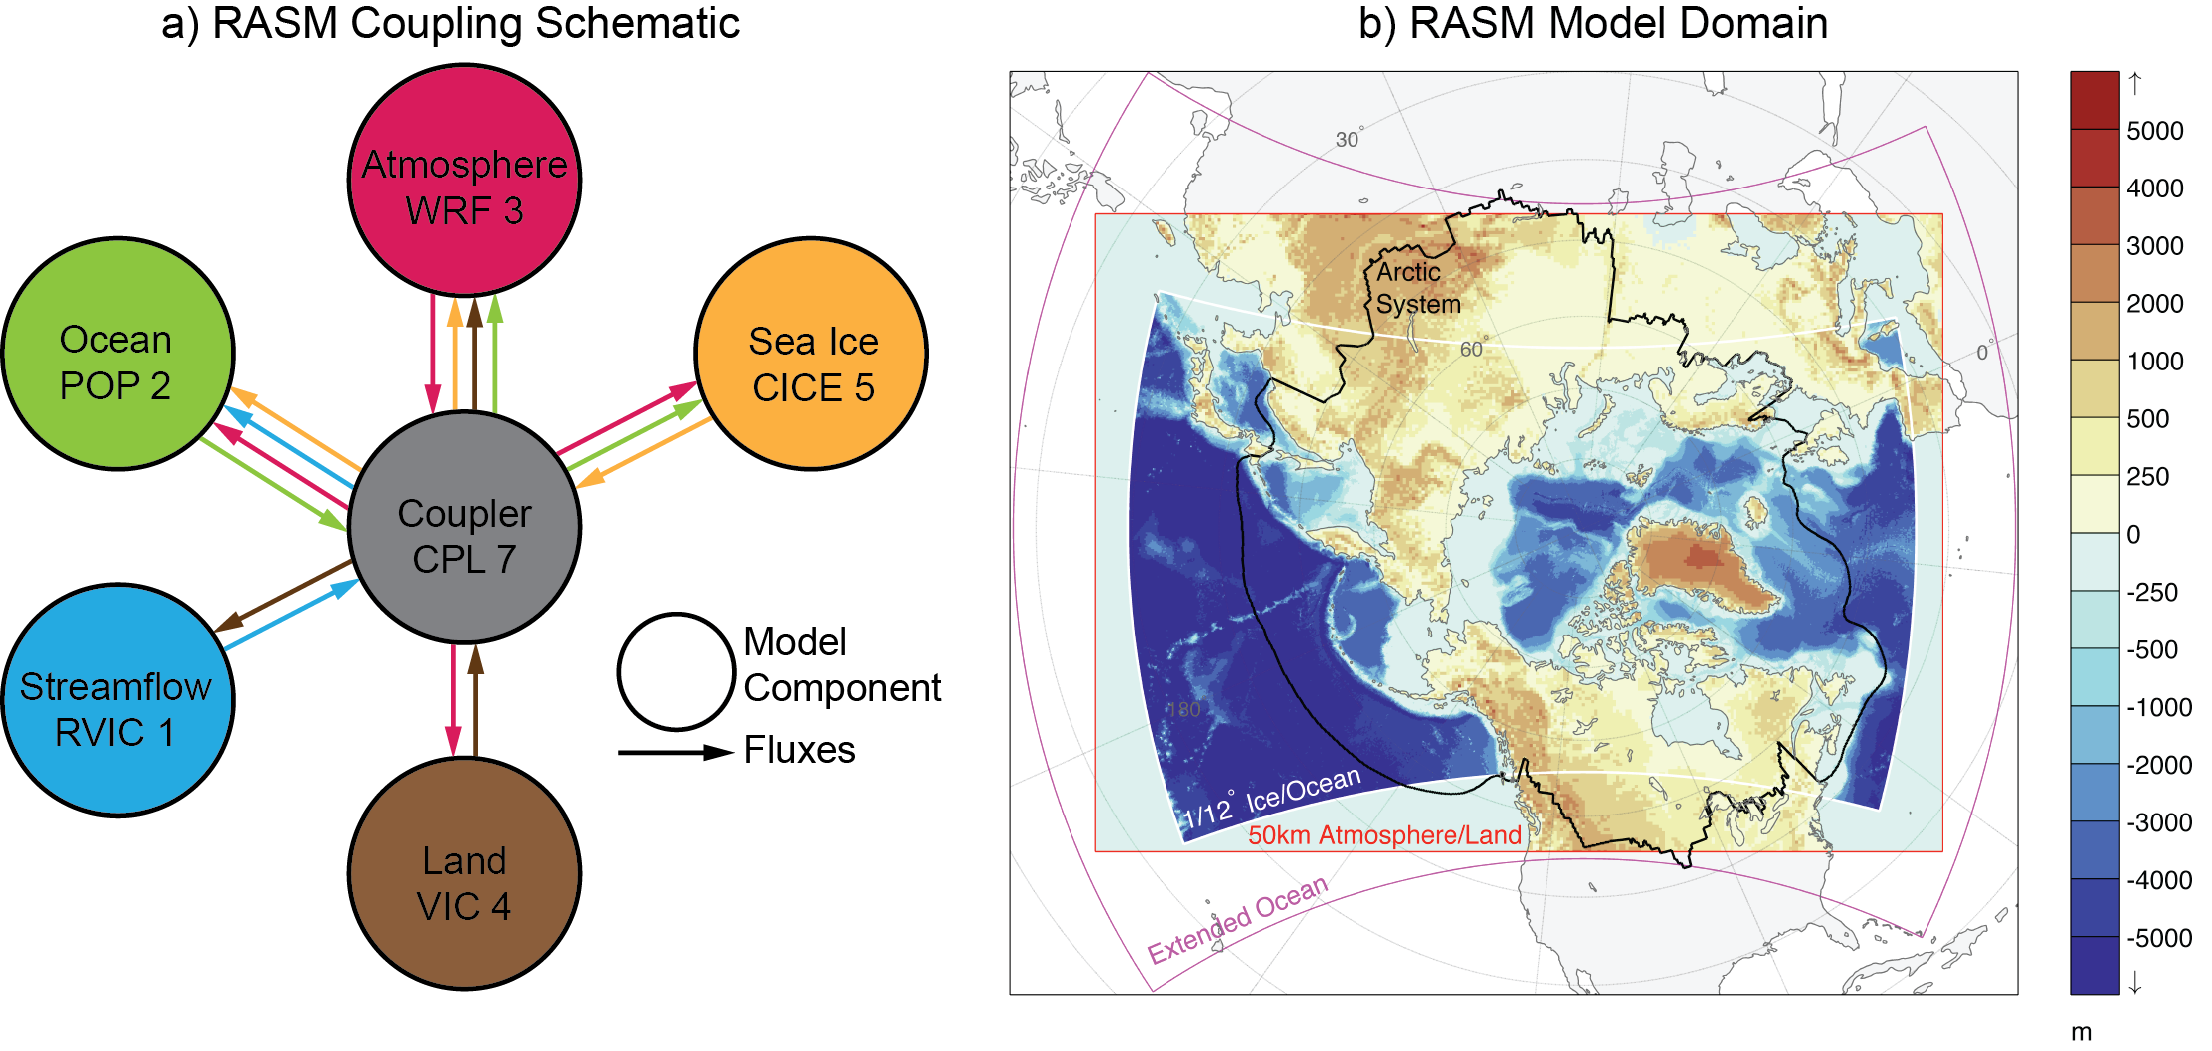
\includegraphics[width=12cm,keepaspectratio]{rasm_schematic_domain}
  \caption{a) Schematic of model configuration in RASM.
  The CPL7 flux coupler passes and receives all fluxes, shown with color coded arrows based on their source model, transferred across model boundaries.
  The component land, atmosphere, ocean, and sea ice models each calculate internal physics apart from the coupler.
  b) RASM model domain.
  There are three main grid domains in RASM, 1/12$^{\circ}$ rotated pole ice/ocean, a 50-km near equal area polar stereographic atmosphere/land/streamflow, and 1/12$^{\circ}$Extended Ocean.
  The color bar represents elevation above or below sea level.
  The black outline designates the greater Arctic Basin.}
  \label{fig:rasm}
\end{figure}

\section{Motivation}

The importance of understanding the Arctic climate system is underscored by the recent and unprecedented observed changes in key climatic processes across the region, and the potential for these changes to impact natural and human activities in coming decades.
Although it is clear that these changes are largely driven by changes in global temperature, the Arctic is expected to play an important role in modulating the rate of warming through a series of radiative, hydrologic, and biogeochemical feedbacks  \citep{Holland_2003}.
Many of the underlying processes that control these feedbacks are either poorly or under represented in global models, which often leads to the misrepresentation the true feedback sensitivity.
global models poorly represent some processes (sea ice, permafrost, runoff, precipitation, circulation)
The development of RASM is motivated by the need to better represent a range of regional processes (e.g. sea ice, permafrost, ice sheets) and feedbacks (e.g. ice-albedo feedback, biogeochemical feedbacks related to permafrost).
RASM seeks to improve the representation of a range of high-resolution processes unique to the polar regions and to provide improved understanding of the coupled relationship between climate system components.

The development and use of a regional climate model, such as RASM, has advantages and disadvantages when compared to global climate model (GCMs).
Most notably, from a computational perspective, regional models are applied over a smaller region than global models, they may be run at higher spatial and temporal resolutions.
Higher resolution is generally thought to improve model representation of certain processes, such as orographic precipitation, coastal processes, and mesoscale processes \citep{Feser_2011}.
Another way to think of how high-resolution regional models are useful is as a ``testbed'' for future global model parameterizations.
As global models trend to higher resolutions, parameterizations related to model dynamics (e.g. ocean eddies, clouds, convective precipitation) will need to be re-evaluated; regional models offer a way to test out new combinations of parameterizations \citep[e.g. ][]{Roberts_2015a,Cassano_2016}.
Regional models must be forced at their lateral boundaries with output from a global model (either reanalysis or a GCM).
In some cases, this can be viewed as a disadvantage of using a regional model since global climate feedbacks are not accounted for.
Conversely, forcing regional models at their boundaries limit the degrees of freedom in the climate system, which can be viewed as an advantage when interpreting the response of new model parameterizations.

\section{Application}

The RASM domain includes the entire Arctic drainage basin and encompasses the historical extent of seasonal sea ice cover.
For the work presented in this dissertation, RASM is applied exclusively over a 50-km near equal-area stereographic grid (Figure \ref{fig:rasm}b).
The individual model components (Figure \ref{fig:rasm}a) in RASM are tightly-coupled in RASM, exchanging flux variables though the flux coupler every 20 minutes.
This coupling configuration is described by \citet{Roberts_2015a}, where the sub-daily coupling frequency is shown to be important in reproducing observed inertial frequencies in the atmosphere-ice-ocean coupling cycle.

RASM version 1.0 was completed in 2015 and since then it has been used in a range of applications.
\citet{Roberts_2015a} used RASM to develop refined ice-ocean-atmosphere coupling scheme at sub-hourly timesteps.
They went on to show how this improvement leads to better simulation of semi-diurnal sea ice drift in RASM and in a GCM.
\citet{Cassano_2016} used RASM to evaluate a range of sea ice, ocean, and atmospheric parameterizations in terms of their impact on radiation biases.
This dissertation (chapters \ref{chap:land_surface}, \ref{chap:streamflow}, and \ref{chap:winter_prec}) represent the existing body of work related to the development and evaluation of the land surface within RASM.

%
\chapter{The Land Surface Climate in the Regional Arctic System Model}
\label{chap:land_surface}

This chapter has been published in its current form in the \textit{Journal of Climate}.
\textcopyright American Meteorological Society.
Used with permission.
The supplemental material for this chapter is provided in appendix \ref{chap:land_surface_sup}.

\hangbibentry{Hamman_2016a}

\section*{Abstract}

The Regional Arctic System Model (RASM) is a fully coupled, regional Earth system model applied over the pan-Arctic domain.
This paper discusses the implementation of the Variable Infiltration Capacity land surface model (VIC) in RASM and evaluates the ability of RASM, version 1.0, to capture key features of the land surface climate and hydrologic cycle for the period 1979-2014 in comparison with uncoupled VIC simulations, reanalysis datasets, satellite measurements, and in situ observations.
RASM reproduces the dominant features of the land surface climatology in the Arctic, such as the amount and regional distribution of precipitation, the partitioning of precipitation between runoff and evapotranspiration, the effects of snow on the water and energy balance, and the differences in turbulent fluxes between the tundra and taiga biomes.
Surface air temperature biases in RASM, compared to reanalysis datasets ERA-Interim and MERRA, are generally less than 2$^{\circ}$C; however, in the cold seasons there are local biases that exceed 6$^{\circ}$C.
Compared to satellite observations, RASM captures the annual cycle of snow-covered area well, although melt progresses about two weeks faster than observations in the late spring at high latitudes.
With respect to derived fluxes, such as latent heat or runoff, RASM is shown to have similar performance statistics as ERA-Interim while differing substantially from MERRA, which consistently overestimates the evaporative flux across the Arctic region.

\section{Introduction}
\label{sec:intro_ch3}

The Regional Arctic System Model (RASM) is a fully coupled regional Earth system model \citep{Roberts_2015a} applied over the pan-Arctic domain (Fig. \ref{fig:domain}a).
The development of RASM has been motivated by the need to improve the representation of critical Arctic processes and feedbacks that affect multidecadal simulations of high-latitude climate, to advance understanding of the coupled interactions between components within the Arctic climate system, and ultimately to better understand climate change at high latitudes.
In RASM, the land surface scheme is the Variable Infiltration Capacity model \citep[VIC; ][]{Liang_1994,Liang_1996}, which is coupled to atmosphere, ocean and sea ice model components via the Community Earth System Model \citep[CESM;][]{Hurrell_2013} flux coupler software infrastructure \citep{Craig_2012}.

\begin{figure}
  \centering
  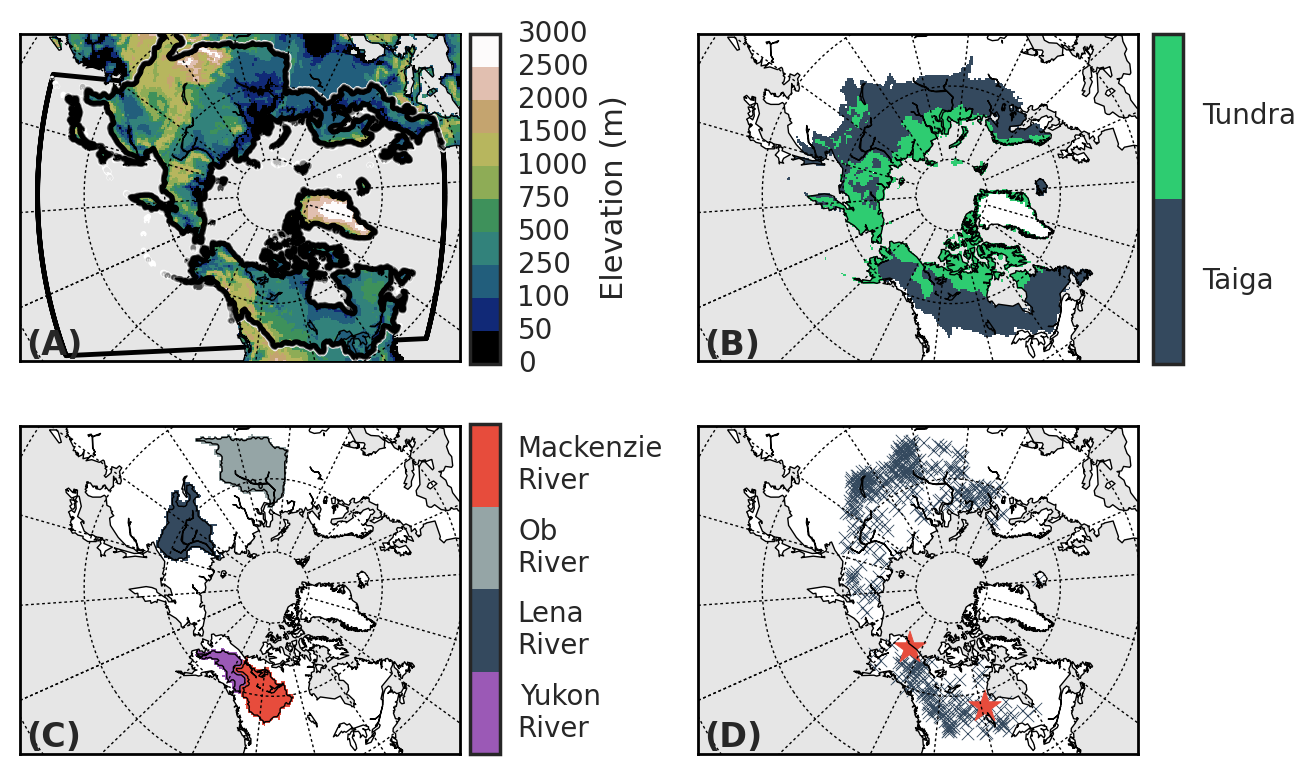
\includegraphics[width=16cm,keepaspectratio]{ch3_Fig1}
  \caption{(a) Domain of the Regional Arctic System Model.
  The 50-km near-equal-area land and atmosphere domain is shown as the outer boundary.
  Shaded areas represent the topographic height for individual land model grid cells.
  The black contour defines the RVIC drainage area over land, and the 1/12$^{\circ}$ inner ocean-ice domain over the ocean.
  (b) The tundra and taiga biomes in the RASM domain.
  (c) The Mackenzie, Ob, Lena, and Yukon River basins.
  (d) The location of R-ArcticNET streamflow gauges (dark blue crosses) and AmeriFlux towers (red stars) used in this analysis.}
  \label{fig:domain}
\end{figure}

We assess the RASM-simulated land surface climate and land-atmosphere coupling in terms of a range of hydrometeorological variables.
We compare fully coupled simulations using RASM version 1.0 to reanalysis, remote sensing, and observation-based datasets.
Our goal in this paper is to establish a baseline for future model development and applications, and to understand the processes that are and are not well represented.

The Arctic land surface plays three primary roles in the global climate system.
First, most of the Arctic land surface has a negative net radiation flux and thus acts as a heat sink, balancing the poleward heat flux from lower latitudes \citep{Fasullo_2008}.
Second, the high albedo in the Arctic during periods of snow cover controls the net shortwave flux in the regional surface energy balance \citep{Flanner_2011}.
Declines in the regional albedo associated with reductions in snow and ice cover therefore contribute to the process of polar amplification \citep{Serreze_2006c}.
Finally, by most accounts, the runoff from the Arctic land surface provides the largest freshwater flux into the Arctic Ocean \citep{Serreze_2006a}.
This flux lowers the salinity in the Arctic Ocean, which is important for sea ice development and is a driver of coastal, regional, and global ocean currents originating in the Arctic Ocean \citep{Morison_2012,Serreze_2006a}.

The land surface hydroclimate in the pan-Arctic region has been extensively studied using offline (uncoupled) hydrologic model simulations.
For example, \citet{Slater_2007} forced five uncoupled land surface models with the ECMWF reanalysis called ERA-40 over the pan-Arctic drainage area.
They cited intermodel differences of up to 30\% in the partitioning of precipitation into evapotranspiration and runoff.
They also noted that most models struggled to capture the winter baseflow behavior, deficiencies that were partially corrected, in some of the models, by adjusting the soil parameterizations.
\citet{Adam_2007} and \citet{Tan_2011} used uncoupled implementations of VIC to investigate twentieth-century changes in annual and seasonal hydrologic fluxes in the Arctic.
Frequently, uncoupled simulations are used to develop new model physics and to improve land surface process representations \citep{Bonan_2011,Bowling_2004,Bowling_2010,Cherkauer_2003,Swenson_2012}.
These studies have been useful in evaluating the model representations of hydrologic processes such as streamflow or evapotranspiration, but have not accounted for coupled land-atmosphere feedbacks.

The development of coupled land-atmosphere and Earth system models has been an important advance in our understanding of hydrometeorology.
Regional and global coupled land-atmosphere models offer a tool to understand how feedbacks between model components propagate changes in individual elements.
Notable examples of this can be found in numerous studies at high and middle latitudes that have shown the importance of antecedent soil moisture and surface albedo in seasonal climate forecasts \citep{Beljaars_1996,Betts_2004,Dominguez_2006,Koster_2004}.
Studies such as these highlight the importance of developing and evaluating land surface processes within a coupled model framework.

In this paper we describe the land surface component coupled within RASM, and evaluate the baseline behavior and performance of the RASM land surface scheme.
Section \ref{sec:models_ch3} provides a brief overview of RASM and the land surface model VIC.
Section \ref{sec:data_ch3} describes the model simulations and comparison data used in this analysis.
Section \ref{sec:results_ch3} presents the results from our analysis, comparing RASM simulated spatial fields to reanalysis and observation-based data products.
Section \ref{sec:discussion_ch3} presents a discussion of our results, using streamflow observations to constrain the partitioning of the hydrologic fluxes.
Section \ref{sec:discussion_ch3} also compares RASM surface fluxes directly to surface observations at selected flux towers, assessing the model's ability to simulate the observed surface energy balance and diurnal cycle.
Finally, section \ref{sec:conclusions_ch3} states our conclusions and outlines the future applications and development intended for the RASM model.

\section{Model description}
\label{sec:models_ch3}

\subsection{RASM}

RASM is a high-resolution, regional, coupled Earth system model that has been developed to improve the representation of critical Arctic process and feedbacks that affect multidecadal simulations of climate in the pan-Arctic domain.
RASM version 1.0 uses the Community Earth System Model (CESM) coupling infrastructure \citep[CPL7; ][]{Craig_2012,Roberts_2015a} and is composed of five component models:

\begin{enumerate}
  \item The Weather Research and Forecasting (WRF) Model \citep{Skamarock_2008} is an atmospheric mesoscale meteorological model. \citet{DuVivier_2016} and \citet{Cassano_2016} provide a detailed description of the WRF model, version 3.2, as it is applied in RASM. Temperature and winds in the top 20 levels of WRF are spectrally nudged to scales larger than approximately 3400 km with nudging linearly ramped from no nudging at level 20 to a nudging strength of 0.0003 s-1 (nudged toward boundary conditions every 55 min) at level 40 \citep{Glisan_2013,Skamarock_2008}.
  \item The Parallel Ocean Program model \citep[POP; ][]{Smith_2010} is a general circulation ocean model. \citet{Roberts_2015a} provide a description of the application of POP, version 2, within RASM.
  \item The Los Alamos Sea Ice model \citep[CICE; ]{Hunke2015} is widely used in regional and global climate simulations. \citet{Roberts_2015a} provide a description of the application of CICE, version 5, within RASM.
  \item The streamflow routing model used is an adapted version of a linear routing model frequently used to route streamflows from VIC output \citep[RVIC; ][]{Lohmann_1996,Lohmann_1998b}. \citet{Hamman_2016b} provide a description of RVIC, version 1.0, as it is applied in RASM.
  \item The Variable Infiltration Capacity model \citep[VIC; ][]{Liang_1994,Liang_1996} is a macroscale hydrologic model. A more detailed description of VIC is provided in section \ref{sec:vic}.
\end{enumerate}

In RASM version 1.0, the land, atmosphere, and runoff components are configured on a 50-km near-equal-area North Pole stereographic grid.
The ocean and sea ice models are configured on a 1/12$^{\circ}$ rotated stereographic grid.
Each model exchanges fluxes with the coupler every 20 minutes \citep{Roberts_2015a}.

\subsection{VIC}
\label{sec:vic}

VIC is a semidistributed hydrologic model that solves the water and energy balance equations at the land surface.
VIC represents subgrid variability in vegetation and topography through a mosaic-style statistical tiling scheme.
Infiltration capacity is nonlinearly distributed \citep{Zhao_1980} and flow from the upper layer is driven by gravity to the lower layers according to \citep{Campbell_1974}.
Base flow is generated from the bottom soil layer and recedes nonlinearly as a function of soil moisture \citep{Dumenil_1992,Todini_1996}.
VIC does not consider direct interactions between neighboring cells, instead assuming that surface and subsurface runoff reach the channel before leaving the grid cell.
In RASM, runoff fields are passed to the flux coupler and are then routed to the Arctic Ocean using RVIC.

When run in energy balance mode, as it is in RASM, VIC uses an iterative process to determine the land surface temperature that minimizes the surface energy balance error \citep{Liang_1999}.
Accumulation and ablation of the snowpack are modeled using a quasi-two-layer snow model, consisting of a thin surface layer and a thicker pack layer \citep{Andreadis_2009,Cherkauer_1999}.
The full energy balance is computed for the surface layer, which exchanges fluxes with the atmosphere, while the pack layer is treated as a reservoir for mass and energy (cold content).
Change in snow water equivalent is the net result of snow, rain, throughfall, sublimation (or condensation), and melt.
Intercepted snow accumulates as a function of the leaf area index and canopy temperature \citep{Storck_2002}.
Snow albedo decays as a function of time and season \citep{Andreadis_2009}.

As an uncoupled hydrologic model, VIC has been applied at global and continental scales \citep{Maurer_2001,Nijssen_1997,Nijssen_2001} including numerous pan-Arctic hydrologic studies \citep{Adam_2007,Slater_2007,Su_2005,Tan_2011}.
VIC has also been coupled to prognostic atmospheric models, such MM5 \citep{Zhu_2009}, to provide lower boundary conditions over land.

RASM uses a modified implementation of VIC, version 4.0.4 (available at https://github.com/UW-Hydro/VIC/releases/tag/VIC.4.0.4).
Extensive structural changes to the VIC source code were required to allow coupling with other RASM component models via the flux coupler, but changes to the physical core of the model were limited.
The VIC physics used within RASM differs from the standard release version 4.0.4 in the following four major ways:

\begin{enumerate}
  \item Vegetation-dependent broadband albedo for snow: VIC typically treats snow-covered vegetation as a completely covered snow surface with a broadband albedo for new snow of 0.85. In early RASM simulations, this led to significant positive biases in surface albedo and consequent negative biases in net shortwave radiation and surface air temperature, especially in coniferous vegetation types with a canopy. In the RASM version of VIC, we have added a vegetation-dependent broadband albedo parameter to address this issue. The updated broadband albedos are taken from \citet{Barlage_2005}, who combined MODIS-derived snow cover and albedo products to define a maximum snow-covered broadband albedo product at 0.05$^{\circ}$ resolution for each University of Maryland land cover type \citep{Hansen_2000}.
  \item Bare-surface albedo: The vegetation cover dataset used in RASM contains only a small amount of bare soil; however, most grid cells designated as bare soil are in actuality ice sheets. Early RASM simulations showed positive biases in net shortwave radiation and therefore surface air temperature in the Canadian archipelago and along the margins of Greenland. These biases were largely corrected by changing the bare-surface albedo from 0.2 to 0.55 to simulate bare ice at high latitudes.
  \item Measurement height: Traditionally, offline versions of VIC assume a globally constant measurement height. The RASM version of VIC uses the height of the lowest WRF model level as the measurement height for atmospheric fields. This height is allowed to vary between grid cells.
  \item Emissivity: In the RASM version of VIC, we have changed the land surface emissivity from 1.0, as is typically used in offline VIC simulations, to 0.97. This change is physically realistic  and ensures that the land surface emissivity is \citep{Prabhakara_1976} consistent with the formulations used by the sea ice and ocean. \citet{Jin_2006} demonstrated that the land surface emissivity has a small, spatially heterogeneous impact on surface soil temperature, net longwave radiation, and the sensible heat flux. Tests using the fully coupled RASM model showed little effect on the land surface temperature.
\end{enumerate}

As applied in RASM, VIC has been configured with a single canopy layer.
The soil parameters were taken from \citet{Sheffield_2006} and were resampled to the 50-km near-equal-area grid using a conservative area remapping technique \citep{Jones_1999}.
Land cover types, LAI, and albedo were resampled to the 50-km near-equal-area grid from the global 0.5$^{\circ}$ VIC input dataset distributed by the University of Washington \citep{Su_2005}, originally derived from \citet{Hansen_2000}.
Table S1 in the supplemental material provides additional details on the land surface parameters used by VIC in RASM.

\subsubsection{Land surface coupling}

In the RASM infrastructure, model components are coupled through the flux coupler CPL7 \citep{Craig_2012}.
Each model component passes all relevant fluxes and states to CPL7, which then aggregates, regrids, and conservatively distributes fluxes to individual model components.
The land-atmosphere coupling is performed at a 20-min time step.
At each coupling time step, the land surface model (VIC) exchanges states and fluxes as detailed in Table S2 of the supplemental material.
RASM includes one-way coupling between the land and ocean components through the freshwater flux.
Runoff and baseflow from VIC are passed via the coupler to the streamflow routing model RVIC, which routes the freshwater flux to coastal ocean grid cells.
\citet{Hamman_2016b} detail the coupling of the RVIC and POP models.

\subsection{Methodology and data}
\label{sec:data_ch3}

\subsubsection{Model simulations}

Uncoupled VIC simulations, run at an hourly time step, were forced with prescribed meteorological inputs from \citet{Sheffield_2006}.
These simulations were used for initialization of the RASM land surface states and for isolated evaluation of changes to the scheme to represent snow-covered vegetation albedo (see section 2b).
Uncoupled simulations were run within the RASM infrastructure using a prescribed atmosphere to ensure that the VIC physics and configurations were identical to the fully coupled simulations.
Initial model states were based on a 31-yr, uncoupled VIC simulation (January 1948 through August 1979).
Using the model state at the end of this period, VIC was run in uncoupled mode for an additional 29 years [September 1979 through December 2008, limited by the period covered by the \citet{Sheffield_2006} dataset; this dataset is referred to herein as $S2006$].
Results from the later 29-yr period will be referred to as $VIC_{S2006}$.

Fully coupled RASM simulations were run for 34 years (September 1979 through December 2014).
The land surface initial state was the same as for the $VIC_{S2006}$ simulation.
This paper discusses the results of two fully coupled, baseline RASM simulations using different atmospheric boundary conditions.
The first was forced with ERA-Interim \citep{Dee_2011} and the other with NCEP's CFSR \citep{Saha_2011}.
These simulations will be referred to hereafter as $RASM_{ERA}$ and $RASM_{CFSR}$, respectively, or collectively as RASM.

\subsubsection{Comparison datasets}
\label{sec:datasets}

Much of the Arctic region is sparsely populated and has few in situ monitoring stations compared to lower latitudes.
The choice of comparison data products used in this paper reflects the need to combine model-simulated reanalysis products with remote sensing and in situ observations to assess the land surface climate of the region.
Table S3 in the supplemental material outlines each of these datasets along with their spatiotemporal characteristics.
All gridded datasets were regridded to the RASM land-atmosphere 50-km near-equal-area grid.

Reanalysis products offer model-simulated estimates of land and atmosphere states and fluxes constrained by observations.
In areas where assimilated observations are sparsely distributed, reanalysis results are more dependent on the reanalysis model than on the assimilated observations.
We used ERA-Interim \citep[also referred to hereafter as ERA; ][]{Dee_2011} and NASA's Modern-Era Retrospective Analysis for Research and Applications \citep[MERRA; ][]{Rienecker_2011} reanalysis products for comparison with RASM land surface fluxes and states.
\citet{Lindsay_2014} have shown that these are two of the best performing reanalysis products in the Arctic region in terms of surface air temperature, precipitation, and radiative fluxes.

Gridded observations of surface air temperature and precipitation suffer from similar sampling problems as reanalysis products but provide a crucial benchmark for model evaluation apart from results of other models.
We use reanalysis datasets that have undergone significant bias correction based on gridded surface observations \citep{Adam_2006,Sheffield_2006}.
We will refer to the \citet{Adam_2006} dataset as A2006.
For these datasets, the reanalysis is solely used to construct the daily variability while the monthly-mean temperature and precipitation are derived from observations.
Both datasets have undergone correction for solid precipitation gauge undercatch and the A2006 dataset has been further adjusted for orographic effects.
For the $S2006$ dataset, precipitation and surface air temperature were bias corrected using the Climate Research Unit (CRU) Time Series (TS) version 2.0, Global Precipitation Climatology Project (GPCP), and Tropical Rainfall Measuring Mission (TRMM) products, and shortwave and longwave radiation were bias corrected using NASA's monthly surface radiation budget (SRB) product.
We use empirically upscaled flux tower observations of sensible and latent heat from \citet{Jung_2011}, referred to herein as J2011, to compare to the model simulated turbulent fluxes.
The J2011 dataset uses machine learning to upscale site-level turbulent heat fluxes based on vegetation, climate, and meteorological predictors.

In situ observations of streamflow offer a unique opportunity for assessing the aggregate water balance over watersheds.
We use the Regional, Electronic, Hydrographic Data Network for the Arctic Region (R-ArcticNET) streamflow database \citep{Lammers_2001} to compare to RASM simulated streamflow.
We selected 379 streamflow gauge locations of the 5688 sites available in the database (Fig. \ref{fig:domain}d).
Sites were selected based on two criteria: first, only sites with at least one complete year of streamflow observations between 1980 and 2014 were chosen (with the year starting in September); second, basin masks were delineated using a 1/16$^{\circ}$ flow direction dataset \citep{Wu_2011} and only sites with a basin area within 10\% of the upstream area reported by R-ArcticNET were used.

Satellite observations of snow cover extent and albedo provide the ability to assess the domain-wide behavior of surface processes.
We use the National Snow and Ice Data Center (NSIDC) Northern Hemisphere Equal-Area Scalable Earth Grid (EASE-Grid 2.0) weekly snow cover extent, version 4 dataset \citep{Brodzik_2013} to compare to RASM simulated snow cover and the global surface albedo product \citep[GlobAlbedo; ][]{Muller_2012} to evaluate surface albedo.

\subsubsection{Approach to model comparison and validation}

Coupled land-atmosphere models, like RASM or reanalyses, are merely ``virtual realities'' and are useful as far as they allow us to explore the coupled processes in the physical climate system \citep{Betts_2004}.
Our approach to assessing the performance of RASM in simulating high-latitude land surface climate has been to select a wide range of comparison datasets (see section \ref{sec:datasets} and Table S3) that provide insight into the underlying processes and behavior of the climate system.
Ultimately, we are interested in the processes that the model simulates and not the exact replication of the climate in any of the chosen comparison datasets.
After all, the uncertainty in spatially distributed observed climatological variables, such as precipitation, is poorly quantified and the spread among individual datasets can be large.
Furthermore, some of the variables of interest (Table S4 in the supplemental material) are simply not measured at a sufficient number of locations to allow for the construction of a spatially gridded dataset (e.g., sensible and latent heat).
In these cases, we turn to point observations (e.g., flux towers) or model predictions (e.g., reanalysis), even though we know that these have their own challenges of representativeness.
None of the datasets used here provided explicit estimates of measurement error or model uncertainty.
Lacking quantifiable measurement error and uncertainty statistics, we have cited estimates published in existing literature, with the goal of putting our comparisons with RASM simulated variables in perspective.

We provide summarized analysis of the annual cycle using two sets of spatial masks.
First, we summarize variables related to the surface energy budget in RASM (see Fig. \ref{fig:energy_cycle}), distinguishing between the tundra and taiga biomes \citep{Olson_2001} (Fig. \ref{fig:domain}b).
Observation-based studies have identified the important and marked differences in land-atmosphere interactions between these biomes \citep{Beringer_2005,Chapin_2000a,Chapin_2000b} and we have therefore used these masks to highlight RASM's performance across different surface types.
Second, we summarize variables related to the hydrologic cycle using masks representing the Mackenzie, Ob, Lena, and Yukon River basins (see Fig. \ref{fig:water_cycle}), delineated using the \citet{Wu_2011} flow direction raster dataset (Fig. \ref{fig:domain}c).

We exclude coastal grid cells from our analysis and discussion because the model datasets tend to report mixed ocean-land states and fluxes, which are not directly comparable with ground observations.
We have also left out discussion of the land surface climate and model performance over the Greenland ice sheet and surrounding polar ice caps for two reasons: 1) there is a lack of distributed and reliable measurements of temperature and precipitation, and 2) the version of RASM that we are using in this study did not include an explicit representation of land ice.
Last, the differences between $RASM_{ERA}$ and $RASM_{CFSR}$ are much smaller than the differences between RASM and the comparison datasets (e.g., see Fig. \ref{fig:temp_maps}).
For this reason, the remainder of the figures in this paper will exclude the $RASM_{CFSR}$ simulation.
All figures in the supplemental material include both RASM simulations.

\section{Results and model evaluation}
\label{sec:results_ch3}

\subsection{Surface air temperature}

Surface air temperature is a function of the surface net radiation, turbulent heat exchange with the atmosphere, and atmospheric dynamics.
Figure \ref{fig:temp_maps} shows spatial maps of RASM-simulated seasonal and annual averaged surface air temperatures across the model domain, compared to the ERA, MERRA, and $S2006$ datasets.
RASM exhibits a zonal gradient in surface air temperatures that is steepest in the winter and in northern Eurasia.
Summer surface air temperatures are more homogeneous with nearly the entire domain experiencing temperatures greater than 0$^{\circ}$C.
Annual average temperatures are less than 0$^{\circ}$C in the tundra and ice-covered regions and near or greater than 0$^{\circ}$C over the taiga and midlatitudes.

\begin{figure}
  \centering
  \includegraphics[width=16cm,keepaspectratio]{ch3_Fig2}
  \caption{Seasonal and annual surface air temperature statistics for September 1989-August 2014.
  (top) $RASM_{ERA}$ averages (bottom-left color bar); (second row) $RASM_{ERA}$ std dev (bottom-center color bar); and (next four rows, from top to bottom) $RASM_{ERA}$ biases compared to $RASM_{CFSR}$, $S2006$, ERA, and MERRA (bottom-right color bar).}
  \label{fig:temp_maps}
\end{figure}

RASM's annual surface air temperature biases, compared to all of the datasets in Fig. \ref{fig:temp_maps}, are relatively low across most of the domain, generally with absolute values of less than 2$^{\circ}$C.
The smallest biases occur in spring and summer.
At the highest latitudes in North America and eastern Siberia, the spring season positive temperature differences are between +2$^{\circ}$ and +6$^{\circ}$C and are most likely related to early seasonal snowmelt, although they are smaller when compared to ERA than to $S2006$.
During fall and winter, RASM exhibits larger surface air temperature biases compared to the other datasets.
The extent and magnitude of these biases suggest better agreement among the comparison datasets during fall and winter than during spring and summer.
In western Siberia, a strong cold bias of between -6$^{\circ}$ and -8$^{\circ}$C is related to a negative bias in downward longwave radiation (discussed in section 4b).
The combination of moderate warm biases in the warm season and strong cold biases in the cool season results in a seasonal cycle with a larger amplitude than reanalysis and observations, accompanied by steeper transitions in the shoulder seasons, especially in fall (Fig. \ref{fig:energy_cycle}).

\begin{figure}
  \centering
  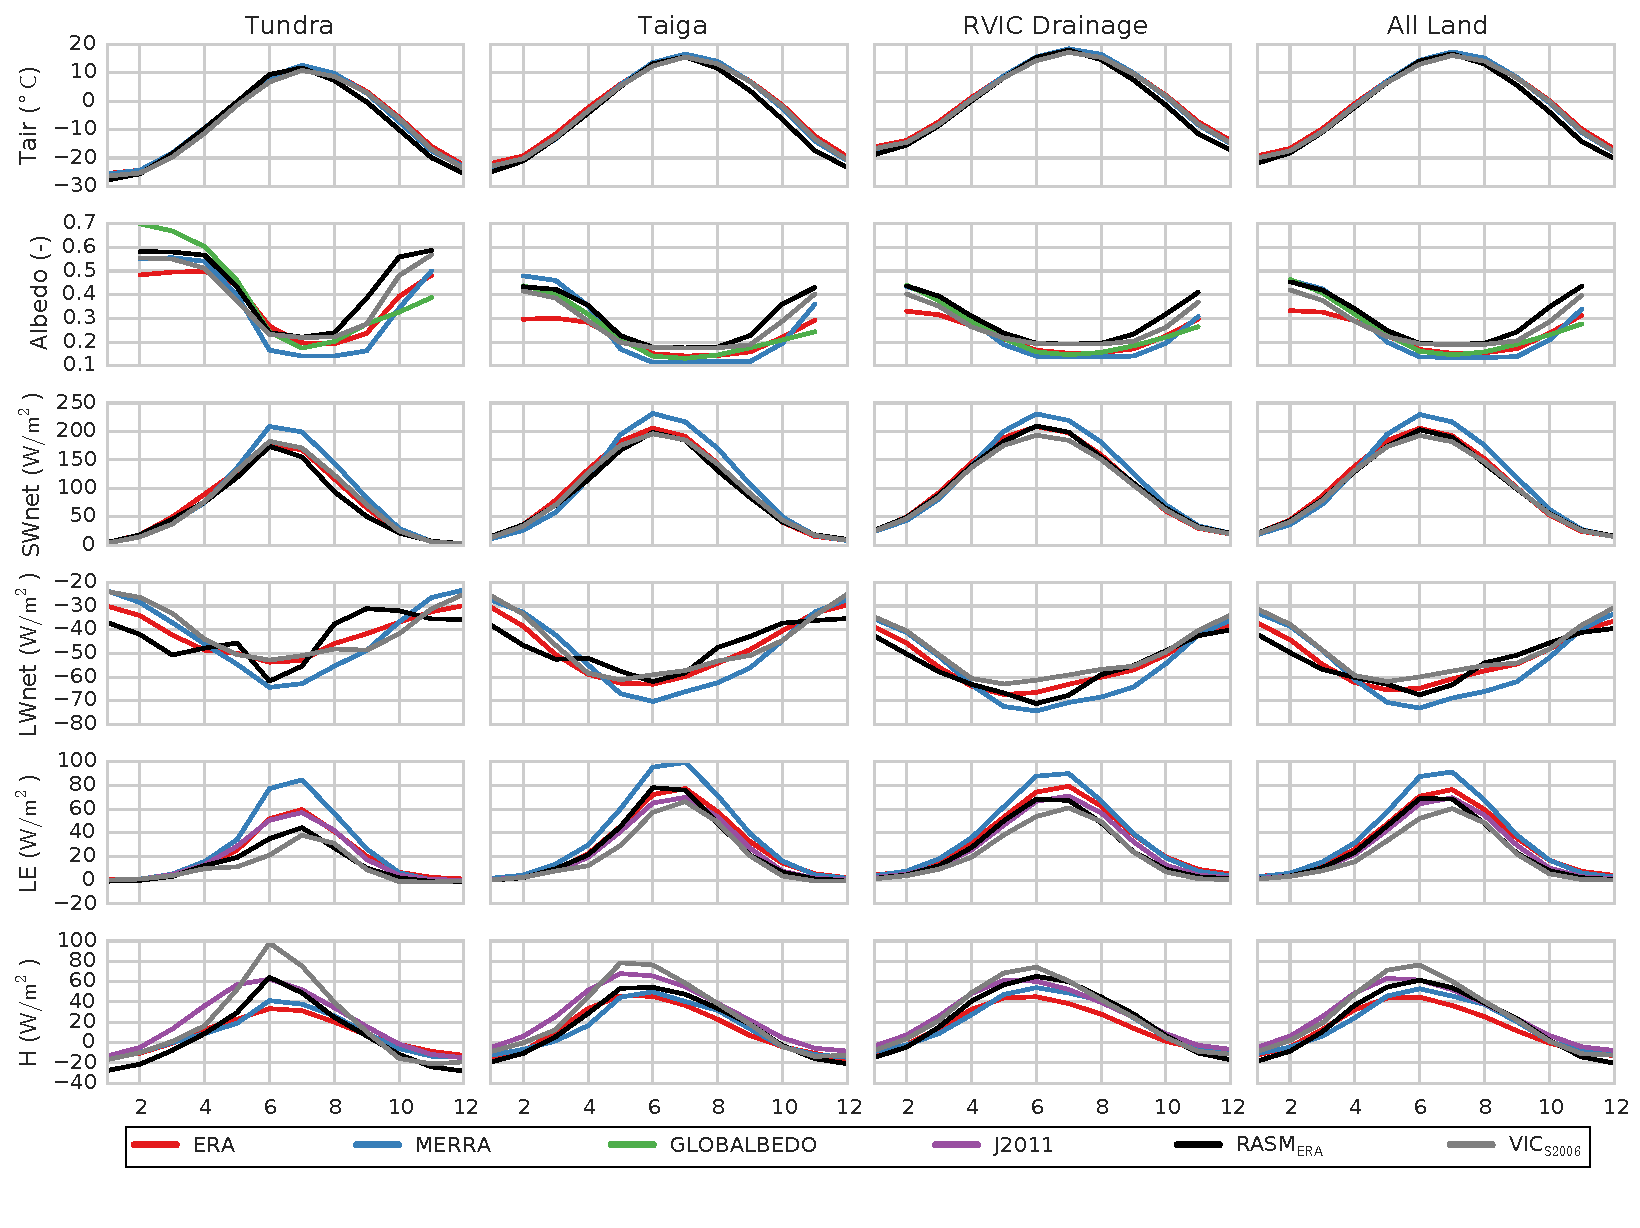
\includegraphics[width=16cm,keepaspectratio]{ch3_Fig3}
  \caption{Average annual cycles of surface air temperature (Tair), albedo, net shortwave radiation (SWnet), net longwave radiation (LWnet), latent heat (LE), and sensible heat (H) for tundra, taiga, the RVIC drainage, and the full model domain for the time period of September 1989-August 2014.}
  \label{fig:energy_cycle}
\end{figure}

\subsection{Radiative fluxes}

The annual cycle of downward shortwave radiation has a large amplitude at high latitudes, with some polar regions receiving less than 30 $W m^{-2}$ in the winter and more than 300 $W m^{-2}$ in the summer.
While clear-sky downward shortwave radiation is only a function of season and latitude, the downward shortwave radiation at the surface also depends on cloud amount and details of the cloud microphysics, which depend on interactions between the atmospheric model boundary layer, microphysics, and radiative transfer schemes.
In RASM, midlatitudes receive 30-50 $W m^{-2}$ more downward shortwave than in ERA, MERRA, and $S2006$, while higher latitudes generally receive less, especially in summer (Fig. S1 in the supplemental material).
In general, the biases in downward radiation in RASM result from too few clouds over midlatitude land areas throughout the year.
The nature of these biases is discussed in detail by \citet{Cassano_2016}.

Reflected shortwave radiation is controlled by the surface albedo, which in the Arctic is mainly determined by the presence or absence of snow.
In the spring, when much of the region is still snow covered, downward shortwave radiation increases rapidly.
Much of this radiation is reflected due to the high albedo of the snow-covered land surface.
RASM captures the difference in cold season albedos between the taiga and tundra, with typical values of 0.4 and 0.6 respectively (Fig. \ref{fig:energy_cycle}).
Compared to the GlobAlbedo product, model simulated surface albedos from RASM, $VIC_{S2006}$, and ERA each have cold season differences that can be as large as +0.25.
Furthermore, all models tend to simulate an early and exaggerated increase in autumn albedo.

Downward longwave radiation is a function of cloud amount, cloud microphysics, and atmospheric temperature and humidity.
Downward longwave radiation is largest in the summer and at midlatitudes (Fig. S3 in the supplemental material).
In the fall and winter seasons at high latitudes, RASM has less downward longwave radiation than ERA, MERRA, and $S2006$, which is driven in part by the cold biases shown in Fig. \ref{fig:temp_maps}, but also contributes to these differences \citep{Cassano_2016}.
The negative downward longwave radiation biases at lower latitudes are mainly due to RASM simulating too few clouds over land areas despite the warm air temperature bias in this region in summer.
Upward longwave radiation is solely a function of the radiative temperature of the land surface, and follows a spatial pattern that is similar to the surface air temperature (Fig. S4 in the supplemental material).
The negative bias in upward longwave in Siberia is reflective of the cold bias in this area.

The combination of downward shortwave and downward longwave radiation is referred to as the total downward radiation and shown in Fig. \ref{fig:drad_maps}.
Total downward radiation has a large seasonal amplitude and a strong zonal gradient, with winter minima at high latitudes less than 150 $W m^{-2}$, and summer maxima at midlatitudes more than 700 $W m^{-2}$.
Compared to ERA and $S2006$, RASM has positive biases at midlatitudes and negative biases at high latitudes, a combination of the previously discussed biases in downward shortwave and longwave radiation.

\begin{figure}
  \centering
  \includegraphics[width=16cm,keepaspectratio]{ch3_Fig4}
  \caption{Seasonal and annual total downward radiation statistics for September 1989-August 2014.
  (top) $RASM_{ERA}$ averages (bottom-left color bar); (second row) $RASM_{ERA}$ std dev (bottom-center color bar); and (next three rows, from top to bottom) $RASM_{ERA}$ biases compared to $S2006$, ERA, and MERRA (bottom-right color bar).}
  \label{fig:drad_maps}
\end{figure}

Net radiation is the difference between total downward radiation and the sum of upward longwave radiation and reflected shortwave radiation.
At high latitudes, average annual net radiation is negative (from -30 to -50 $W m^{-2}$) across most of the pan-Arctic region in the winter (Fig. \ref{fig:nrad_maps}).
Over most of the domain, the net radiation at the surface in RASM is within 15 $W m^{-2}$ of $VIC_{S2006}$, MERRA, and ERA.

\begin{figure}
  \centering
  \includegraphics[width=16cm,keepaspectratio]{ch3_Fig5}
  \caption{Seasonal and annual net radiation statistics for September 1989-August 2014.
  (top) $RASM_{ERA}$ averages (bottom-left color bar); (second row) $RASM_{ERA}$ std dev (bottom-center color bar); and (next three rows, from top to bottom) $RASM_{ERA}$ biases compared to $VIC_{S2006}$, ERA, and MERRA (bottom-right color bar).}
  \label{fig:nrad_maps}
\end{figure}

\subsection{Turbulent fluxes}

Surface turbulent heat fluxes are perhaps the least constrained flux variables in coupled land-atmosphere models.
Estimates of sensible and latent heat flux from the MERRA and ERA reanalysis products are computed entirely within the reanalysis land surface model and are not directly constrained by data assimilation.
\citet{Lindsay_2014} highlight that point in their intercomparison of seven reanalysis products over the pan-Arctic domain, citing intermodel variations in the seasonal sensible and latent heat fluxes in some regions on the order of 50 $W m^{-2}$.
RASM and the reanalysis products simulate a regional maximum latent heat flux across the taiga in the summer (Fig. \ref{fig:energy_cycle}).
In RASM, the sensible heat flux in the midlatitudes is from +10 to +40 $W m^{-2}$ greater than in ERA and MERRA during summer.
RASM latent heat fluxes tend to be lower than both ERA and MERRA but are closer to the empirical estimates of J2011 (Fig. S5 in the supplemental material).

The annual cycle of the latent heat flux is largely driven by the seasonal cycle of net shortwave radiation.
In the winter season (DJF), the latent heat flux is nearly zero across the entire RASM domain (Fig. S5).
The latent heat flux is largest in the summer over the taiga, with a seasonal averaged latent heat flux near 80 $W m^{-2}$.
The spatial distribution of the seasonally averaged latent heat flux varies substantially among models (e.g., RASM, MERRA, and ERA).
Local differences in the simulated latent heat flux can be as large as 50 $W m^{-2}$.
Averaged over the taiga, the summer season (JJA) latent heat flux is more than +20 $W m^{-2}$ larger in MERRA than in the RASM, ERA, or J2011 datasets.
As discussed below, these differences in the latent heat flux are consistent with the differences in the partitioning of evapotranspiration and runoff.

The sensible heat has a more distinct zonal gradient than the latent heat flux, with the largest sensible heat fluxes in the southern portions of the domain (Fig. S6 in the supplemental material).
This gradient is stronger in RASM than in MERRA, ERA, or J2011.
The differences in the sensible heat flux when compared to MERRA and ERA are closely related to the differences in total downward radiation.
RASM simulated winter season sensible heat is negative over most of the domain, especially over the high latitudes.
A negative sensible heat flux represents an energy flux from the atmosphere to the land surface or heating of the land by the atmosphere.
The ERA, MERRA, and J2011 datasets agree with this behavior although the spread among the models is as large as 30 $W m^{-2}$.
Intermodel differences in the sensible heat flux can be as large as the differences in the latent heat flux.
In the case of RASM, the biases have a zonal structure that is likely tied to biases in downward radiation rather than vegetation.

In the tundra and taiga regions, the sensible heat flux characteristically peaks about a month earlier than the latent heat flux.
This process is primarily due to large amounts of downward radiation over a mostly snow-covered land surface, which inhibits evapotranspiration \citep{Betts_2001}.
Figure \ref{fig:energy_cycle} demonstrates that RASM follows this asymmetry in the turbulent fluxes.

\subsection{Hydrologic fluxes}

Figure \ref{fig:prec_maps} shows the spatial distribution of RASM precipitation.
The spatial pattern of precipitation in the Arctic is highly heterogeneous.
Significant portions of the domain receive less than 300 $mm yr^{-1}$ (0.8 $mm day^{-1}$), while some coastal and midlatitude regions receive over 1500 $mm yr^{-1}$ (4.1 $mm day^{-1}$).
Precipitation is largest in the summer across most of the pan-Arctic region.
In most cases, RASM simulates larger amounts of orographic precipitation (e.g., west coast of North America) compared to MERRA and ERA, likely as a result of its higher spatial resolution and therefore greater ability to resolve topography.


\begin{figure}
  \centering
  \includegraphics[width=16cm,keepaspectratio]{ch3_Fig6}
  \caption{Seasonal and annual precipitation statistics for September 1989-August 2014.
  (top) $RASM_{ERA}$ averages (bottom-left color bar); (second row) $RASM_{ERA}$ std dev (bottom-center color bar); and (next four rows, from top to bottom) $RASM_{ERA}$ biases compared to $S2006$, ERA, MERRA, and A2006 (bottom-right color bar).}
  \label{fig:prec_maps}
\end{figure}

We compared the basin average precipitation for four basins (Fig. \ref{fig:domain}c) with four reanalysis and observation based datasets (Fig. \ref{fig:water_cycle}).
RASM effectively captures the seasonal cycle of precipitation, with the largest precipitation amounts in the summer season.
While most of the datasets show similar amounts of accumulated cold-season precipitation, $S2006$ stands out as being particularly dry, leading to less snow accumulation.
The annual cycle of runoff in the Arctic is driven by spring snowmelt and summer precipitation.
RASM captures this pulse in melt season runoff in each of the basins shown in Fig. \ref{fig:water_cycle}.
For $RASM_{ERA}$, $VIC_{S2006}$, ERA, and MERRA there are significant differences in seasonality of basin-averaged runoff compared to R-ArcticNET with the spring freshet in most datasets preceding the observations by 1-2 months.

\begin{figure}
  \centering
  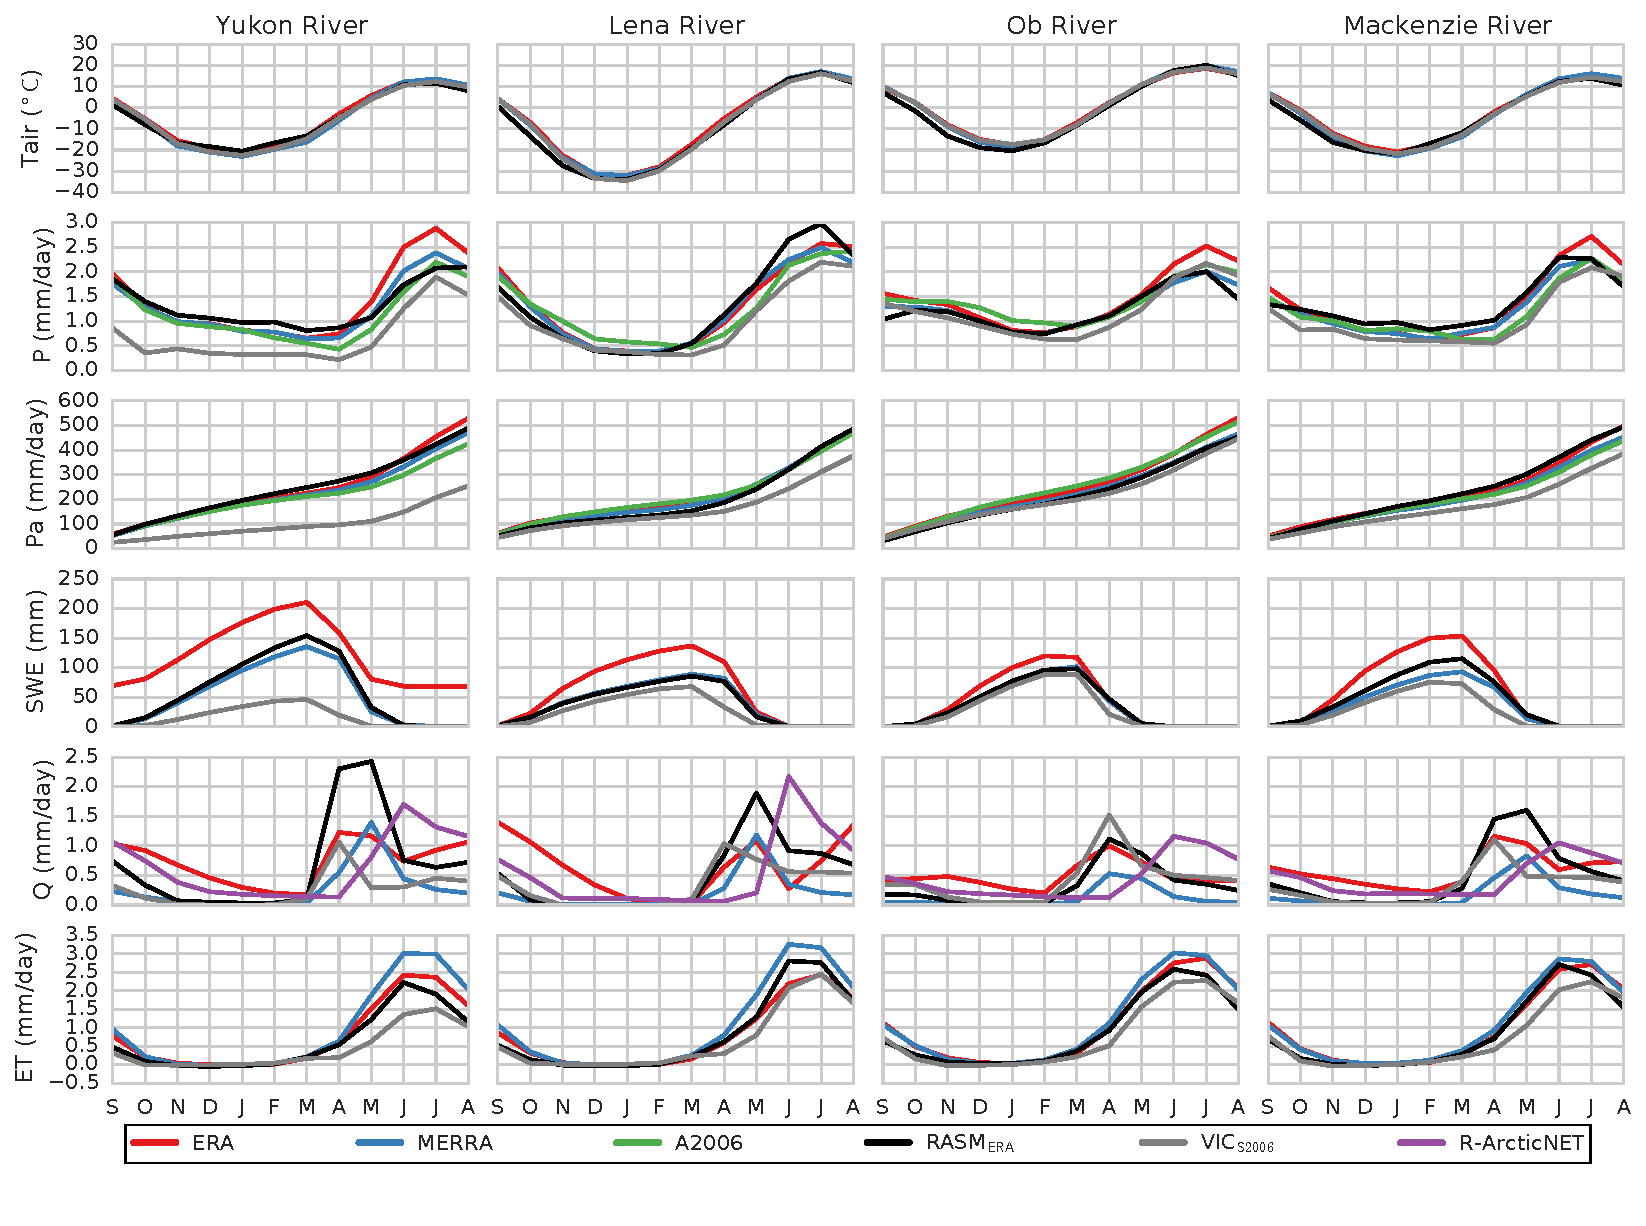
\includegraphics[width=16cm,keepaspectratio]{ch3_Fig7}
  \caption{Average annual cycles of Tair, precipitation (P), accumulated precipitation (Pa), snow water equivalent (SWE), streamflow (Q), and evapotranspiration (ET) for four of the largest river basins in the RASM domain for the time period of September 1989-August 2014.}
  \label{fig:water_cycle}
\end{figure}

\subsection{Snow}

Winter and spring snow cover influence the regional and global climate through increased surface albedo, the latent heat required for melting and sublimation, and the freshwater flux into the Arctic during late spring and summer.
Basin-averaged snow water equivalent (SWE) in RASM shows seasonal accumulation and ablation patterns that are similar to MERRA and ERA.
Basin-averaged differences correspond largely to differences in cool season precipitation (Fig. \ref{fig:water_cycle}).
The annual cycle of basin-averaged snow water equivalent in RASM is generally closer to that of MERRA than ERA.

Figure \ref{fig:snow} compares snow cover north of 50$^{\circ}$N (defined in RASM and the reanalysis products as grid cells with average SWE >1 mm) to the National Snow and Ice Data Center weekly snow cover data product.
Note that the uncertainty in the satellite estimated snow cover extent is on the order of 5\%-10\% in the spring \citep{Brown_2011}.
Additional uncertainty is introduced in our analysis through the comparison between model snow cover derived using a grid cell average SWE threshold and remote sensing estimates of snow cover.
RASM simulated snow cover extent north of 50$^{\circ}$N reaches a maximum by the start of January and a minimum by the end of June.
RASM's increase in snow-covered area in fall closely follows the MERRA and NSIDC datasets and its onset of spring melt matches NSIDC.
However, RASM simulations show a shorter ablation period, especially at high latitudes in North America and eastern Siberia between May and June, where the retreat of snow-covered area in RASM precedes satellite observations by about 15 days.
Accompanying this more rapid retreat of high-latitude snow cover is a warm bias in May and June in those regions.
Increase in snow-covered area in the $VIC_{S2006}$ simulation lags by more than 10 days, whereas the decrease precedes that of the other dataset due to less precipitation in $S2006$ compared to the other datasets (see also Figs.
\ref{fig:water_cycle} and \ref{fig:snow}).


\begin{figure}
  \centering
  \includegraphics[width=16cm,keepaspectratio]{ch3_Fig8}
  \caption{Number of snow-covered days per year for (top left) RASM and (top right) NSIDC.
  (bottom left) Difference between numbers of snow-covered days per year in (top).
  (bottom right) Annual cycle of snow-covered area north of 50$^{\circ}$N.
  Time period is September 1989-August 2014.}
  \label{fig:snow}
\end{figure}

\section{Discussion}
\label{sec:discussion_ch3}

In uncoupled land surface simulations, models are frequently evaluated on the basis of their ability to capture key terms in the hydrologic cycle, such as snow water equivalent, streamflow, soil moisture, and evapotranspiration.
These models are often calibrated using objective functions that target only one or two of these variables.
In many cases, these calibrations, or parameter selection techniques, achieve good statistical representation of the target variables without additional assessment of the remaining fluxes and states in the model.
In the process of developing the VIC-WRF coupling in RASM, we have found it necessary to take a holistic approach to assess model performance.
Our focus has been on improving the representation of individual processes and understanding how individual processes contribute to the climate system rather than achieving an optimal calibration.

The land surface is coupled to the atmosphere via three primary mechanisms: surface radiation exchange, turbulent heat flux exchange, and the partitioning of precipitation into evapotranspiration and runoff.
Our analysis of the surface energy budget in the RASM domain indicates that differences in the downward radiation forcings (±50 $W m^{-2}$), compared to reanalysis and $S2006$, may be large enough to affect the land surface model performance.
An example of this is in western Siberia during the winter and fall when RASM shows less downward longwave radiation than the reanalysis products, leading to local surface air temperature biases between -4$^{\circ}$ and -8$^{\circ}$C as compared to ERA.

The largest control on the terrestrial surface energy budget is the surface albedo.
During winter and spring, the tundra is snow-covered and its albedo can be 6 times higher than in the adjacent taiga \citep{Chapin_2000b} where vegetation with much lower albedo protrudes through the snow.
Early RASM simulations did not include a vegetation-dependent maximum snow albedo, resulting in cool season albedos in vegetated areas that were much higher than observations.
These high values in surface albedo were accompanied by negative surface air temperature biases over much of the tundra and taiga that were as large as -10$^{\circ}$C.
Applying a vegetation-dependent maximum snow albedo resulted in a lower surface albedo (Fig. \ref{fig:albedo_maps}) and reduced the surface air temperature bias throughout the cool season.
These results extend the findings of \citet{Viterbo_1999}, who reduced the snow-covered vegetation albedo from 0.8 over the taiga to 0.2 in ECMWF's global forecast model resulting in a reduction of surface air temperature bias from more than -8$^{\circ}$C to less than -2$^{\circ}$C.

\begin{figure}
  \centering
  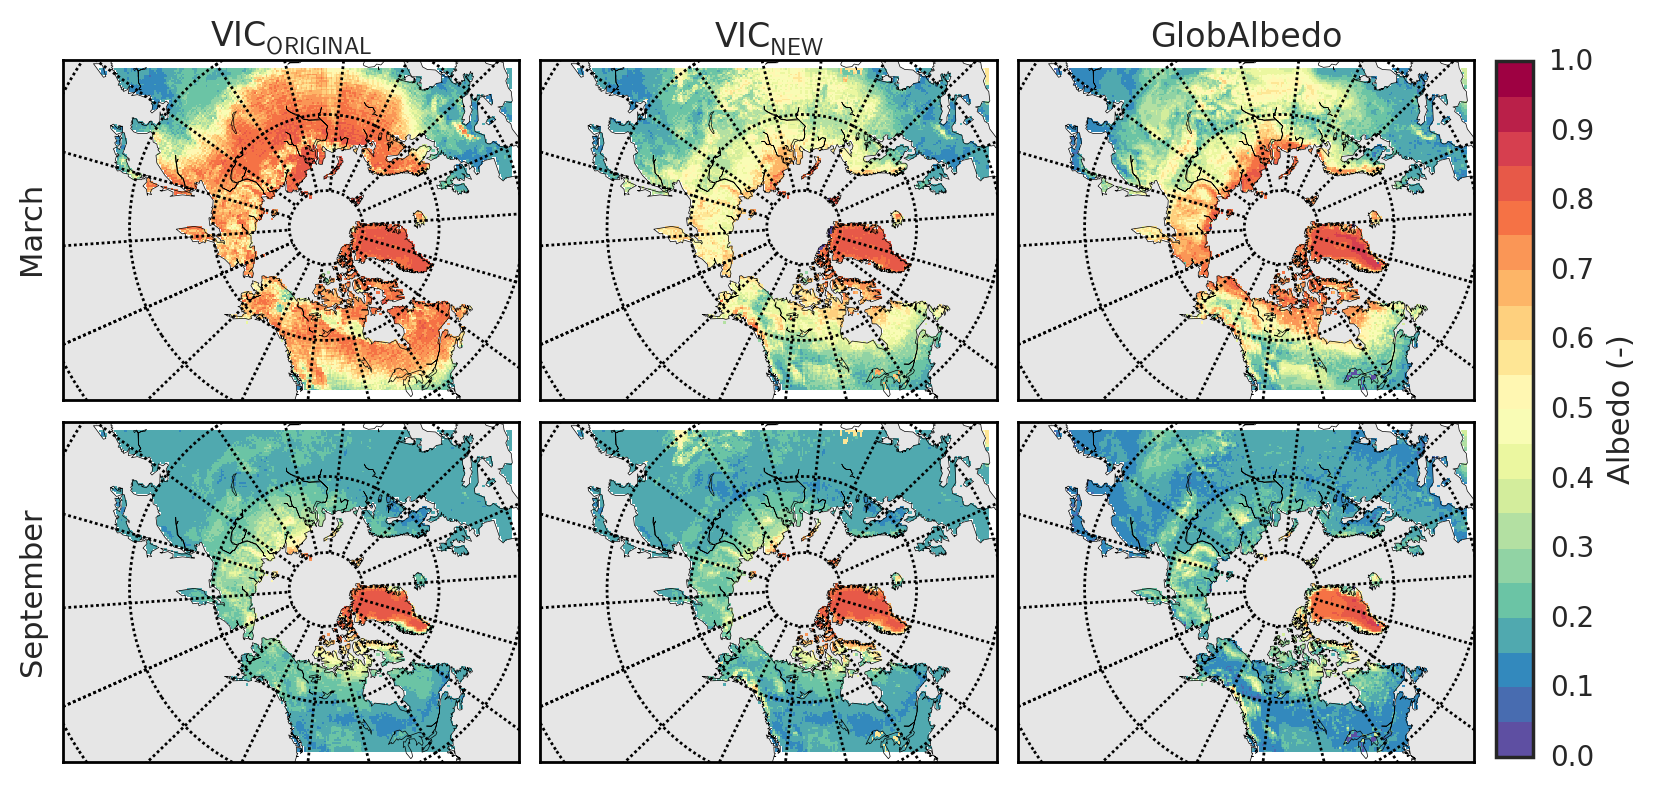
\includegraphics[width=16cm,keepaspectratio]{ch3_Fig9}
  \caption{Surface albedos for (top) March and (bottom) September for (left) the original VIC albedo schemes, (center) the albedo schemes used in RASM (e.g., VICNEW), and (right) the GlobAlbedo remote sensing product.
  Time period is 1998-2007.}
  \label{fig:albedo_maps}
\end{figure}

Observational studies, such as \citet{Beringer_2005}, have shown that the tundra and taiga biomes partition the warm season turbulent heat fluxes differently.
Across the taiga regions, we expect Bowen ratios to be much greater than one in the spring and near one in the summer (Fig. \ref{fig:bowen}).
In the tundra regions, we expect growing season (JJA) Bowen ratios of less than one.
In the taiga, RASM captures the spring peak in the Bowen ratio with an average value of 1.13 and the decline in summer with an average value of 0.76 (see Table S5 in the supplemental material).
In the tundra during the summer, RASM tends to have a higher than expected Bowen ratio of 1.55.
During the fall, turbulent fluxes tend to be small and RASM, ERA, and MERRA register negative Bowen ratios, resulting from a negative sensible heat flux.
Comparing RASM, ERA, and MERRA to the spatial patterns found in the empirical estimates of J2011, we find that ERA and MERRA tend to have much lower Bowen ratios across much of the domain during all three seasons.
This is particularly apparent during the spring and summer months in the high latitude tundra portions of the domain, where RASM and J2011 both show Bowen ratios near or above 1.0 while ERA and MERRA are consistently below 1.0.

\begin{figure}
  \centering
  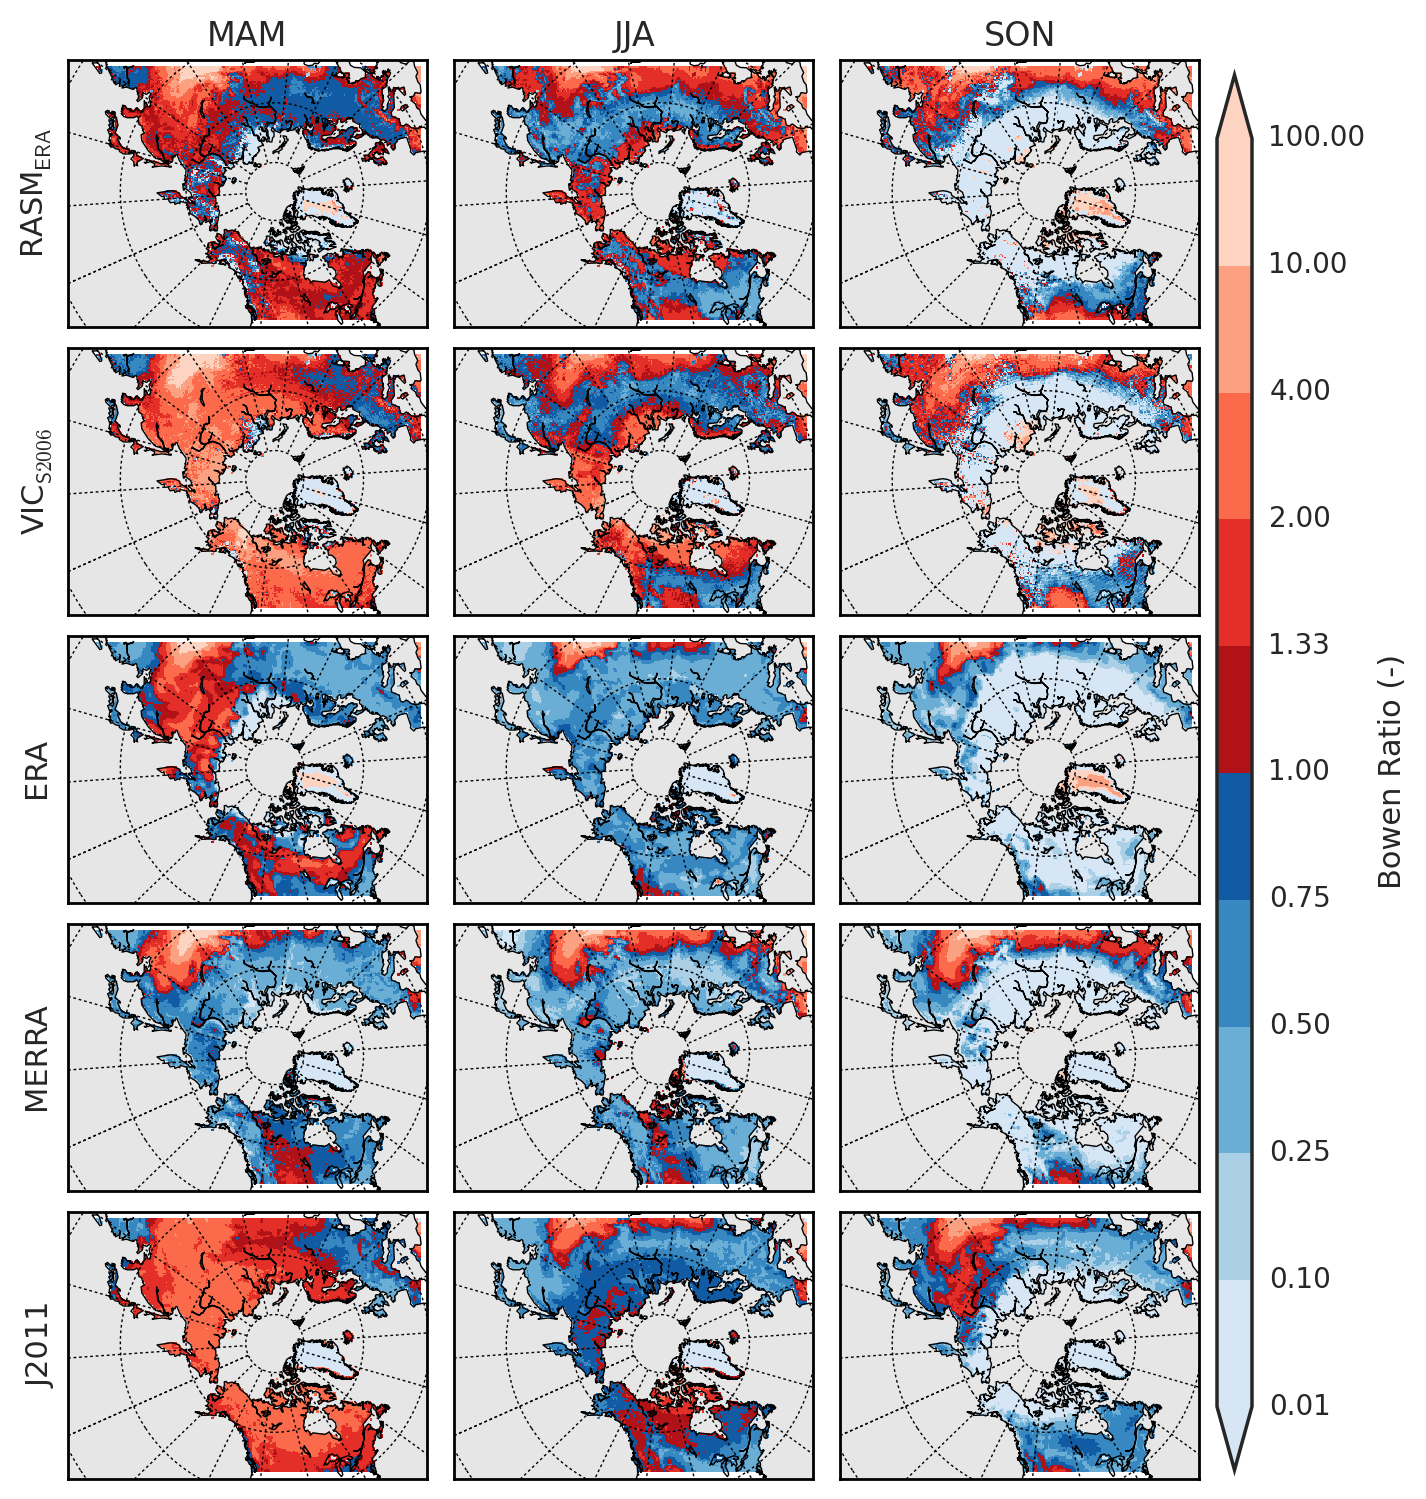
\includegraphics[width=14cm,keepaspectratio]{ch3_Fig10}
  \caption{Spring, summer, and fall Bowen ratios for $RASM_{ERA}$, $VIC_{S2006}$, ERA, MERRA, and J2011 for the time period of September 1989-August 2014.}
  \label{fig:bowen}
\end{figure}

The turbulent heat fluxes, along with heat storage, balance net radiation at the surface.
The partitioning of the turbulent heat fluxes between latent heat and sensible heat is a function of the stability of the boundary layer and the availability of mobile liquid water at or below the surface.
In the pan-Arctic region, the seasonal and diurnal cycles of the sensible and latent heat fluxes vary considerably by land cover types.
To highlight RASM's ability to simulate the turbulent heat fluxes, we compared the diurnal cycles at two flux tower locations to the nearest RASM grid cells.
This analysis serves to demonstrate that RASM simulates the diurnal cycle with close resemblance to point observations, particularly with respect to the magnitude and timing of the diurnal cycle and the relative importance of the individual fluxes.
Figure \ref{fig:diurnal_cycle} shows the observed July-averaged (1994 and 1995) diurnal cycle at the Boreal Ecosystem Atmosphere Study \citep[BOREAS; ][]{Sellers_1997} Old Black Spruce \citep{Barr_2006} and the Happy Valley, Alaska \citep{Eugster_2000}, flux tower locations (Fig. \ref{fig:domain}d) compared to the RASM-simulated diurnal cycle at the nearest grid cell location.
The BOREAS and Happy Valley sites are representative of the taiga and tundra locations, respectively.
RASM's diurnal temperature range (DTR) at the BOREAS site is similar to the observed DTR (about 10$^{\circ}$C) despite being about 2$^{\circ}$C colder on average.
At the tundra site, however, the RASM-simulated DTR (about 5$^{\circ}$C) is much smaller than the observed 9$^{\circ}$C.
At both locations, net radiation is similar to the observations in terms of magnitude and diurnal timing and is mostly determined by the atmospheric forcing of downward radiation.
The timing of the diurnal cycle of the latent heat and the sensible heat fluxes in RASM is similar at both the taiga and tundra sites, and the differences in the magnitude are typically less than 40 $W m^{-2}$.
Averaged over the month of July, RASM and observed Bowen ratios at the BOREAS site were 0.89 and 1.27, respectively, and were 0.88 and 0.69 at the Happy Valley site.

\begin{figure}
  \centering
  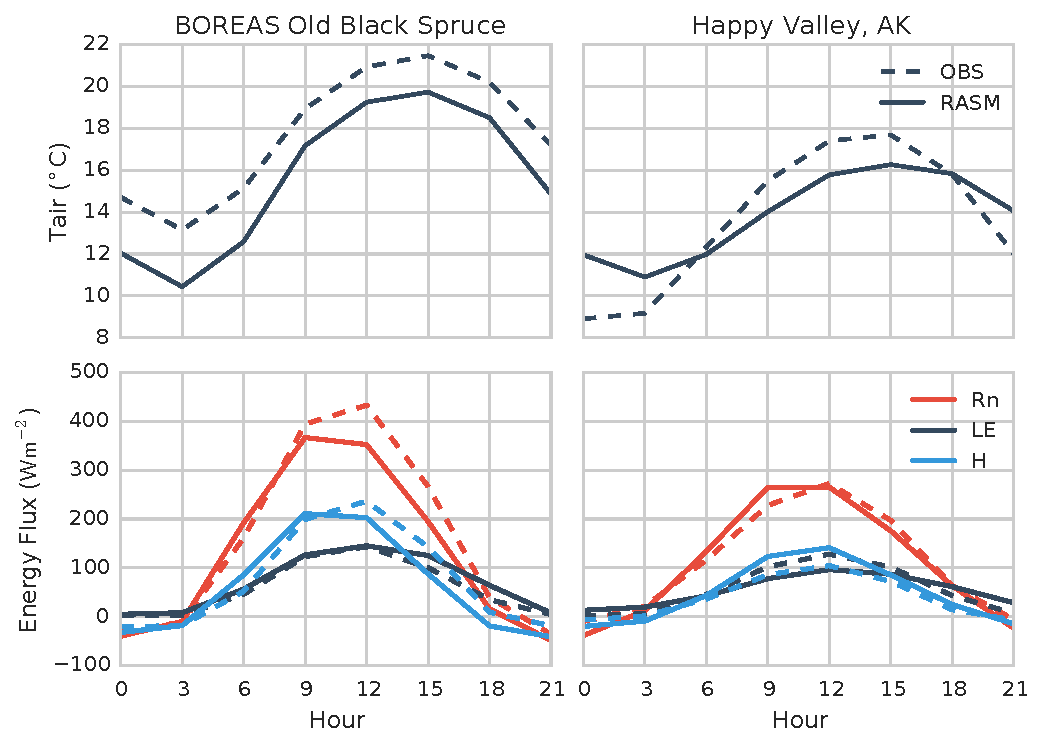
\includegraphics[width=12cm,keepaspectratio]{ch3_Fig11}
  \caption{(top) Averaged diurnal cycle of Tair and (bottom) net radiation (Rn), LE, and H for July at the (left) BOREAS Old Black Spruce and (right) Happy Valley, Alaska, flux tower locations based on observations (OBS; dashed line) and RASM (solid line).
  RASM results are based on the simulated values at the nearest grid cell location.
  Time period is July 1994 and 1995.}
  \label{fig:diurnal_cycle}
\end{figure}

On annual time scales, surface and subsurface runoff from the land surface can be thought of as the difference between precipitation and evapotranspiration, assuming no change in storage.
Since we lack the ability to effectively measure evapotranspiration across large areas, in situ observations of streamflow and gridded observations of precipitation enable us to evaluate the overall water balance.
Figure \ref{fig:streamflow_scatter} shows climatological, basin-averaged precipitation, runoff, and runoff ratios from the A2006 precipitation and R-ArcticNET (Fig. \ref{fig:domain}d) runoff datasets and compares these to the same quantities based on $RASM_{ERA}$, $VIC_{S2006}$, MERRA, and ERA.
Compared to A2006 precipitation, $RASM_{ERA}$ has the lowest root-mean-square error (RMSE) and bias of all the models, +0.3 and +0.0072 mm day$^{-1}$ respectively.
$VIC_{S2006}$, which is forced using $S2006$, has a negative bias (-0.34 mm day$^{-1}$) compared to A2006, especially in wetter basins (those with precipitation greater than 1.75 mm day$^{-1}$).
All of the datasets are biased low with respect to runoff compared to R-ArcticNET.
$RASM_{ERA}$ and ERA have the smallest biases, -0.12 and -0.021 mm day$^{-1}$, respectively, while the $VIC_{S2006}$ and MERRA datasets have biases of -0.3 and -0.4 mm day$^{-1}$, respectively.
Although the differences in precipitation between MERRA and A2006 are not large, annual runoff from MERRA is substantially lower than observed at nearly all gauge locations, indicating systemic overestimation of evapotranspiration (and thus the latent heat flux) in MERRA.
This finding aligns with the results shown in Figs. \ref{fig:snow} and \ref{fig:bowen}, in which MERRA is shown to have larger evapotranspiration and latent heat fluxes and smaller Bowen ratios than RASM or ERA.
\citet{Shiklomanov_2006} estimated annual runoff measurement errors in the largest six Eurasian rivers between 1.5\% and 3.5\%.
If we apply these error estimates across the entire R-ArcticNET dataset, we find that measurement errors are about an order of magnitude smaller than the biases shown in Fig. \ref{fig:streamflow_scatter}.
Compared with the combination of A2006 and R-ArcticNET runoff, all models have considerably more scatter in their runoff ratio than they do for runoff or precipitation alone (Fig. \ref{fig:streamflow_scatter}).
RASM, ERA, and $VIC_{S2006}$ overpredict low runoff ratios and underpredict high runoff ratios while MERRA is consistently biased low.


\begin{figure}
  \centering
  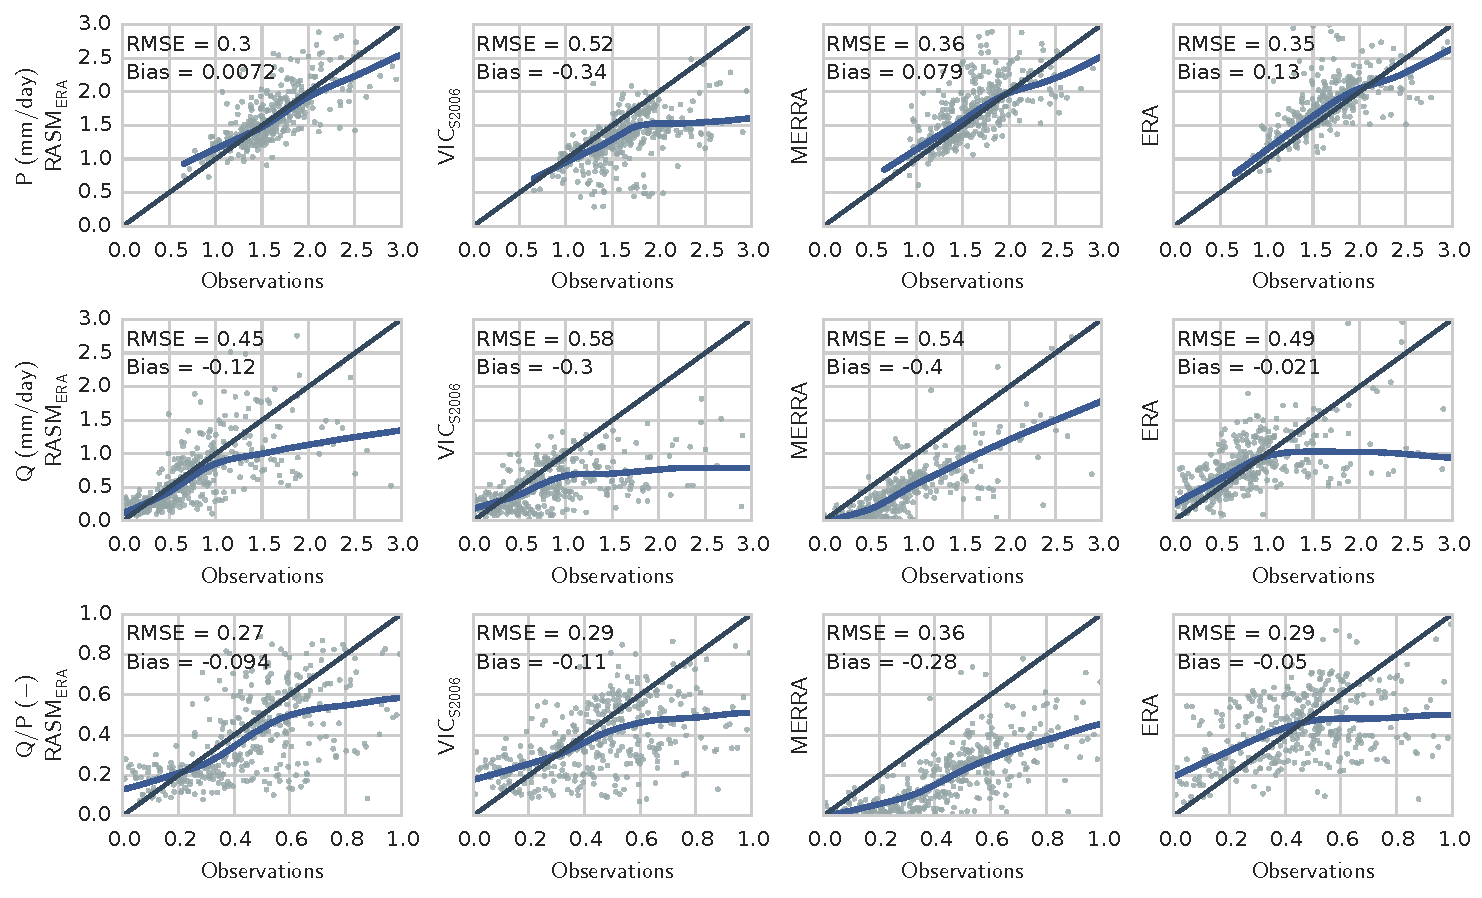
\includegraphics[width=16cm,keepaspectratio]{ch3_Fig12}
  \caption{Comparison of observed P from A2006 and Q from R-ArcticNET to $RASM_{ERA}$, $RASM_{CFSR}$, $VIC_{S2006}$, MERRA, and ERA at 379 individual basins.
  The blue line is a locally weighted scatterplot smoothing (LOWESS) best-fit model.
  The RMSE (mm day$^{-1}$) and bias (mm day$^{-1}$) statistics are shown in the top-left corner of each panel.
  Climatological mean of coincident records between September 1980 and August 2014.}
  \label{fig:streamflow_scatter}
\end{figure}

The energy and water cycles are linked through the latent heat flux.
The partitioning of precipitation into runoff and evapotranspiration is also directly related to the latent heat flux.
We have shown large intermodel differences in the runoff ratio, especially between RASM and MERRA.
RASM and ERA tend to have similar runoff generation behavior on annual time scales and also tend to match the global J2011 dataset well.
Conversely, MERRA tends to have very low runoff ratios and considerably higher latent heat fluxes in the spring and summer compared to J2011.
ERA's annually averaged runoff tends to match observations reasonably well, despite having slightly greater precipitation in the spring and summer \citep[see Fig. \ref{fig:streamflow_scatter} herein; ][]{Lindsay_2014}.
While considering the evapotranspiration flux from MERRA and ERA, it is worth remembering that both models assimilate observations of humidity in the troposphere and thus, by design, eliminate most of the feedback mechanisms between evapotranspiration and precipitation.
This explains in part why MERRA's precipitation is reasonable despite more evapotranspiration than ERA or RASM.

The need to evaluate land surface model performance in a coupled environment is demonstrated by the substantial differences in model results between the coupled and uncoupled VIC simulations ($RASM_{ERA}$ and $VIC_{S2006}$), distinctions that warrant further investigation.
For example, in the coupled environment, biases in atmospheric forcings, such as the cold season negative bias in downward longwave radiation in $RASM_{ERA}$, result in biases at the land surface and feedbacks to the atmosphere through the surface energy budget.
In the uncoupled environment, the atmospheric forcing is prescribed so that most of the land-atmosphere feedback processes are ignored.

\section{Conclusions}
\label{sec:conclusions_ch3}

The development of RASM has been motivated by the need to improve multidecadal climate simulations in the pan-Arctic region and to improve understanding of the coupled climate system.
We coupled the VIC land surface model within the CESM infrastructure and compared land surface fluxes and states to uncoupled simulations, reanalysis datasets and observation-based products to provide a baseline evaluation of the land surface climate in RASM version 1.0.
Based on these comparisons, we have shown that RASM reproduces many important aspects of the Arctic land surface climate, such as the amount and regional distribution of precipitation and its partitioning between runoff and evapotranspiration, the effects of snow on the water and energy balance, and the differences between the main tundra and taiga biomes in simulated turbulent fluxes.
We also compared RASM to the reanalyses ERA and MERRA.
In comparisons with assimilated variables, such as surface air temperature, we found that RASM reproduces the spatial patterns and seasonal cycle well, although there are large local differences and RASM has a larger seasonal amplitude overall.
With respect to derived variables, such as latent heat or runoff, we found that RASM, in comparison to observation-based datasets, performs as well as or better than ERA or MERRA.
We have also shown that there are specific aspects in the land surface component that can be improved.
For example, while the annual cycle of snow-covered area in RASM compares well to satellite observations, the melt progresses faster in the late spring at high latitudes.

The partitioning of the hydrologic fluxes varies among $RASM_{ERA}$, ERA, and MERRA.
For example, $RASM_{ERA}$ and ERA tend to agree on the annual runoff ratio, but demonstrate substantially different seasonal runoff behavior, with RASM simulating a well-defined runoff peak in April or May and ERA simulating a smaller spring runoff peak with more runoff throughout the summer and autumn.
Conversely, MERRA has very low runoff ratios and the largest amount of evapotranspiration.
We have found that these relationships can also be applied to the surface energy budget.
Among $RASM_{ERA}$, ERA, and MERRA, we have found a wide range in the sensible and latent heat fluxes.
MERRA tends to have a larger latent heat flux and a smaller Bowen ratio than $RASM_{ERA}$ and ERA, which is consistent with MERRA's low runoff ratio.

Ongoing development of the RASM land surface and land-atmosphere coupling includes improved treatment of ground heat flux and canopy processes, increased spatial resolution, and coupling of new submodel components including a subgrid glacier model and a dynamic vegetation model.

{\bf Acknowledgments}
This research was supported under U.S. Department of Energy (DOE) Grants DE-FG02-07ER64460 and DE-SC0006856 to the University of Washington, and DE-SC0006178 to the University of Colorado.
Supercomputing resources were provided through the Department of Defense (DOD) High Performance Computing Modernization Program at the Army Engineer Research and Development Center and the Air Force Research Laboratory.
We would also like to thank José Renteria and Kevin Lind for their early contributions to the coupling of VIC within RASM, work that was funded through the DOD user Productivity, Enhancement, Technology Transfer, and Training (PETTT) program.

%
\chapter{The Coastal Streamflow Flux in the Regional Arctic System Model}
\label{chap:streamflow}

This chapter has been submitted in its current form and is currently in review with the \textit{Journal of Geophysical Research: Oceans}.

\hangbibentry{Hamman_2016b}

\section*{Abstract}

The coastal streamflow flux from the Arctic drainage basin is an important driver of dynamics in the coupled ice-ocean system.
Comprising more than one-third of the total freshwater flux into the Arctic Ocean, streamflow is a key component of the regional and global freshwater cycle.
To better represent the coupling of the streamflow flux to the ocean, we have developed and applied the RVIC streamflow routing model within the Regional Arctic System Model (RASM).
The RASM is a high-resolution regional Earth System Model whose domain includes all of the Arctic drainage basin.
In this paper, we introduce the RVIC streamflow routing model, detailing its application within RASM and its advancements in terms of representing high-resolution streamflow processes.
We evaluate model simulated streamflow relative to in-situ observations and demonstrate a method for improving model performance using a simple optimization procedure.
We also present a new, spatially and temporally consistent, high-resolution dataset of coastal freshwater fluxes for the Arctic drainage basin and surrounding areas that is based on a fully-coupled RASM simulation and intended for use in Arctic Ocean modeling applications.
This dataset is evaluated relative to other coastal streamflow datasets commonly used by the ocean modeling community.
We demonstrate that the RASM-simulated streamflow flux better represents the annual cycle than existing datasets, especially in ungauged areas.
Finally, we assess the impact that streamflow has on the coupled ice-ocean system, finding that the presence of streamflow leads to reduced sea surface salinity, increased sea surface temperatures, and decreased sea ice thickness.

\section{Introduction}
\label{sec:intro_ch4}
% [Overview of the Arctic freshwater budget/cycle and the role of streamflow.]
Approximately 11\% of global terrestrial runoff drains into the Arctic Ocean, which holds only 1.4\% of the Earth's salt water \citep{Lewis_2000,Lammers_2001}.
As a result, the Arctic Ocean has the lowest salinity among the Earth's oceans \citep[e.g.][]{Steele_2001}.
Streamflow is the largest contributor of fresh water to the Arctic Ocean as it comprises approximately 38\% of the total freshwater flux entering the Arctic Ocean; the remainder of which consists of direct precipitation (24\%) over the Arctic Ocean, inflow from the Pacific Ocean (30\%), and inflow from the Atlantic Ocean (8\%) \citep{Serreze_2006a}.
The streamflow flux to the Arctic Ocean also has a distinct seasonal cycle.
Across the Arctic region, the annual runoff hydrograph is characterized by a prominent spring freshet, with about two-thirds of the annual runoff volume occurring between April and July \citep{Lammers_2001}.
During the spring and summer months, the fractional contribution of fresh water to the Arctic Ocean from streamflow may be as high as 60\% (uncertainty in this figure is largely the result of uncertainty in the seasonal cycle of the Bering Strait inflow) \citep{Serreze_2006a}.

% [The role of streamflow in ocean/ice dynamics]
Streamflow to the Arctic Ocean plays an important role in coastal ocean dynamics and hydrography, as well as in sea ice formation and melt \citep{Weatherly_1996,Rabe_2011,Fichot_2013}.
Runoff from Arctic river basins is the primary source of buoyancy-driven currents such as the Alaska, Siberian, Norwegian, and East Greenland coastal currents \citep[e.g.][]{Morison_2000,Boyd_2002,Maslowski_2002,McGeehan_2012,Myers_2005}.
Coastal currents play important roles in shelf dynamics and shelf-basin interactions, redistributing both fresh water and heat through mixing \citep[e.g.][]{Carmack_1989,Rudels_1999,Ekwurzel_2001,Maslowski_2014}.
Buoyancy delivered by rivers lowers sea surface salinity (SSS), which increases the freezing (and melting) temperature of sea water, therefore affecting the onset of sea ice formation in winter and melt in spring and summer \citep[e.g.][]{Weatherly_1996}.
Thus, for a warming and freshening Arctic Ocean, increases in the freezing temperature and resulting changes in the onset of freezing may partially buffer regional warming in areas highly influenced by streamflow.
However, the earlier sea ice freeze-up enabled by lower SSS also reduces the amount of heat the upper ocean can lose during the fall, potentially counteracting the impact of freshening on sea ice development \citep{Weatherly_1996,Morison_2012}.
Streamflow is also important for maintaining the stratification of the Arctic Ocean \citep{Nummelin_2015}.
Although warmer water exists at depth in the Arctic Ocean, stratification is maintained by the density gradient between the cold, fresh, mixed layer above and the more saline halocline and Atlantic water layers below \citep{Serreze_2006a}.
This relatively strong pycnocline limits the heat flux into the surface mixed layer from  below.

% [ocean / sea ice specific studies]
The coastal streamflow flux has also been shown to be an important driver of dynamics in coupled ice-ocean models \citep[e.g.][]{Newton_2008,Large_2009,Lique_2015}.
\citet{Newton_2008} applied observed climatological runoff from nine of the largest rivers within the Arctic basin in the Naval Postgraduate School (NPS) Arctic coupled ice-ocean Model (NAME) and used passive numerical flow tracers to track the spatial distribution of runoff.
They found the highest concentration of river runoff along the Siberian coast and identified that freshwater plumes originating as coastal streamflow entered the central Arctic Ocean along topographic boundaries on the ocean floor.
However, they went on to conclude that the relatively coarse spatial resolution of their model (18 km) was a limiting factor in in resolving coastal ocean dynamics and that future studies evaluating the interaction of streamflow in the Arctic Ocean would benefit from higher spatial resolution and improved forcing datasets.
Despite our understanding of the importance of river runoff in Arctic Ocean dynamics, \citet{Nummelin_2015} show that global climate models (GCMs) poorly represent the vertical structure of the Arctic Ocean, with many models failing to accurately reproduce the observed profiles of temperature and salinity in the upper 500 m of the central Arctic Ocean.
They conclude that an accurate representation of the streamflow flux is a key step toward improving the performance of ocean models in GCMs.

% [Arctic Hydrology literature]
Numerous observational and modeling studies have explored the seasonal and inter-annual behavior of Arctic runoff.
\citet{Lammers_2001} compiled the R-ArcticNET database, a regional hydrographic record of mean monthly streamflow observations that included over 3,700 streamflow gauges in the Pan-Arctic region.
The collection of observations in R-ArcticNET was later used by \citet{Shiklomanov_2009} in their investigation of increasing river discharge in the largest Eurasian rivers and by \citet{Tan_2011} in their study of changes in spring snowmelt timing.
\citet{Dai_2009} extended a coastal subset of the R-ArcticNET database through 2007 as part of their study estimating the global streamflow flux.
Several studies \citep{Su_2005,Adam_2007,Slater_2007,Adam_2008,Dai_2009} have used uncoupled land surface models (LSMs) in conjunction with routing schemes to simulate streamflow across the pan-Arctic region.
These studies have led to an improved understanding of the terrestrial hydroclimate in the Arctic and of the response of seasonal streamflow dynamics to changes in climate and water management activities in the Arctic basin.

The Coordinated Ocean-ice Reference Experiments (CORE) Corrected Inter-Annual Forcing (CIAF) Version 2.0, hereafter referred to as $CORE.v2$, is a widely used ocean model forcing dataset that includes coastal streamflow estimates from \citet{Dai_2009} (see section \ref{sec:data_ch4}).
A strength of the $CORE.v2$ dataset is that it includes observed monthly mean streamflow on a global 1$^{\circ}$ x 1$^{\circ}$ grid, blended with model results that are used to fill temporal gaps and to provide streamflow estimates in ungauged areas.
However, this blending approach may also be viewed as a weakness of the dataset insofar as it introduces spatial and temporal discontinuities where and when observations are unavailable.
As we will show in section \ref{sec:results_ch4}, these discontinuities are particularly severe in large ungauged areas such as Greenland and the Canadian Archipelago.

% [Paper overview]
In this paper, we describe the RVIC streamflow routing scheme implemented within the recently developed Regional Arctic System Model (RASM) \citep{Roberts_2015a,DuVivier_2016,Hamman_2016a} to simulate the streamflow flux between the land and ocean model components.
RVIC is named after the routing model that has typically been used with the Variable Infiltration Capacity [VIC] hydrologic model \citep{Liang_1996}.
We introduce the new RVIC streamflow routing model in section \ref{sec:models_ch4}, where we describe its parameterization of high-resolution streamflow routing as well as its coupling within RASM.
Model simulations, and input and comparison data sets are defined in section \ref{sec:data_ch4}.
In section \ref{sec:results_ch4}, we evaluate RVIC-simulated streamflow relative to in-situ observations and compare the regionally aggregated coastal streamflow flux to observation and model-based datasets commonly used by the Arctic ocean and climate modeling communities.
In section \ref{sec:discussion_ch4} we compare two RASM simulations, with and without coastal runoff, to highlight the role and importance of an accurately representation of streamflow in coupled climate simulations in the Arctic region.
In the same section we present a new, spatially- and temporally-consistent, high-resolution dataset of coastal freshwater fluxes for the Arctic drainage basin and surrounding areas that is based on a fully-coupled RASM simulation and intended for use in Arctic Ocean modeling applications.
Finally, in section \ref{sec:conclusions_ch4}, we provide our conclusions and highlight the advancements offered by the RVIC model and the associated coastal streamflow flux dataset.

\section{Models}
\label{sec:models_ch4}

\subsection{RASM}
\label{sec:rasm}
The Regional Arctic System Model is a fully-coupled, high spatial and temporal resolution, regional Earth system model (ESM) applied over the pan-Arctic domain (Figure \ref{fig:rasm_domain}).
The principal goals for the development of RASM are 1) to better understand the interaction between physical systems in the Arctic drainage basin; 2) to advance understanding of past and present states of Arctic climate; and 3) to improve seasonal to multi-decadal prediction capabilities of key climate change indicators in the Arctic.
Model components are coupled using the Community Earth System Model \citep[CESM; ][]{Hurrell_2013} coupled model framework and the CPL7 flux coupler \citep{Craig_2012}.
Below, we provide a brief description of the five component models in RASM version 1.0 (Figure \ref{fig:rasm_coupling_schematic}).
For the purposes of this paper, we are principally concerned with the representation of the coastal streamflow flux and its role in the Arctic Ocean system.
Therefore, our RASM description focuses on the streamflow and ocean model components.
The reader will find additional information regarding the implementation of individual component models in the RASM-specific references cited below.

\begin{figure}
    \centering
    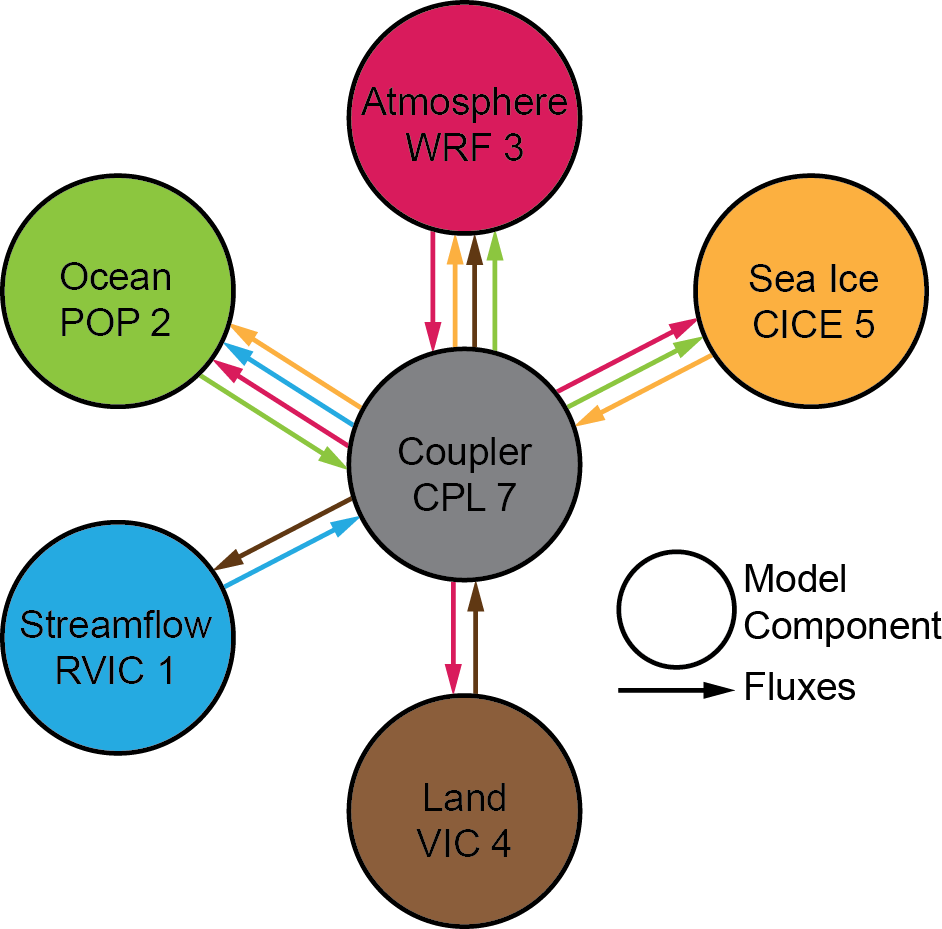
\includegraphics[width=10cm,keepaspectratio]{RASM_coupling_schematic}
    \caption{Coupling schematic for the Regional Arctic System Model. Circles represent model components (e.g. RVIC) and arrows between circles represent flux and state variables shared between components (e.g. streamflow). The colors of the arrows reflect the source of the fluxes and state variables.}
    \label{fig:rasm_coupling_schematic}
\end{figure}

\begin{itemize}
\item CICE: \citet{Roberts_2015a} described the coupling of the Los Alamos Sea Ice Model (CICE) version 4 in RASM.
For this paper, we have upgraded CICE in RASM to version 5 \citep{Hunke2015} and incorporated the high-frequency sea ice coupling configuration described by \citet{Roberts_2015a} as part of the developmental version of RASM.
With this upgrade, we have configured the new version of CICE to use anisotropic sea ice mechanics \citep{Tsamados2013}, level ice melt ponds \citep{Hunke2013}, and perhaps most importantly, a mushy-layer thermodynamics column model of \citet{Turner2015} with a prognostic salinity profile through the sea ice.
\item POP: The Parallel Ocean Program model is a general circulation ocean model \citep{Smith_2010}.
\citet{Maslowski_2012}, \citet{Roberts_2015a}, and \citet{Osinski_2016} provide descriptions of the application of POP version 2, within RASM.
Of particular relevance to this study, POP uses a virtual salinity flux ($VSF$) to represent changes in ocean salinity due to surface fluxes of fresh water (runoff, ice melt, precipitation, and evaporation).
The $VSF$ is the equivalent amount of salt that would have to be added or removed from a model grid cell to obtain the same change in salinity as results from a given freshwater flux.
The virtual salinity flux is calculated as
\begin{equation}
  \label{eq:SaltFlux}
  VSF=-F_w S
\end{equation}

where $F_w$ is the sum of the freshwater fluxes from streamflow, precipitation, evaporation, and sea ice melting and freezing, and $S$ is the reference salinity, which is the surface salinity of the grid cell receiving the freshwater flux.

\item VIC: The Variable Infiltration Capacity model \citep{Liang_1994} is a macroscale land surface hydrology model.
\citet{Hamman_2016a} provide a description of the application of VIC within RASM.
\item WRF: The Weather Research and Forecasting atmospheric model \citep{Skamarock_2007} is a mesoscale meteorological model.
\citet{Cassano_2016} provide a detailed description of the WRF model, version 3.2, as it is applied in RASM.
\item RVIC: The RVIC streamflow routing model is an adapted version of the \citet{Lohmann_1996} linear, source-to-sink routing model frequently used to route the runoff flux from the VIC model.
A complete description of the RVIC model is provided in section~\ref{sec:rvic}.
\end{itemize}

In RASM Version 1.0, the land, atmosphere, and runoff components share a 50-km near-equal-area North Pole stereographic grid mesh.
The ocean and sea ice models share a 1/12$^{\circ}$ rotated sphere mesh (Figure \ref{fig:rasm_domain}).
All model components are coupled at 20-minute intervals.
This high-frequency coupling configuration is described by \citet{Roberts_2015a}, where the sub-daily coupling frequency is shown to be important in reproducing observed inertial frequencies in the atmosphere-ice-ocean coupling cycle.
For this study, we have also improved the simulation of ice-ocean freshwater exchanges, made possible by using mushy-layer sea ice thermodynamics.
In this latest version of RASM, both the sea ice and ocean models use a variable freezing temperature set by a liquidus relation \citep{Turner2015}, rather than a fixed basal ice temperature of -1.8$^\circ$C as is often assumed in fully coupled GCMs \citep [e.g.,][]{Jahn2012a}.
As a result, the freezing temperature of sea water is a function of the ocean salinity at the ice-water interface rather than a constant value, thus significantly improving model physics associated with the ice-ocean salinity flux.

\begin{figure}
    \centering
    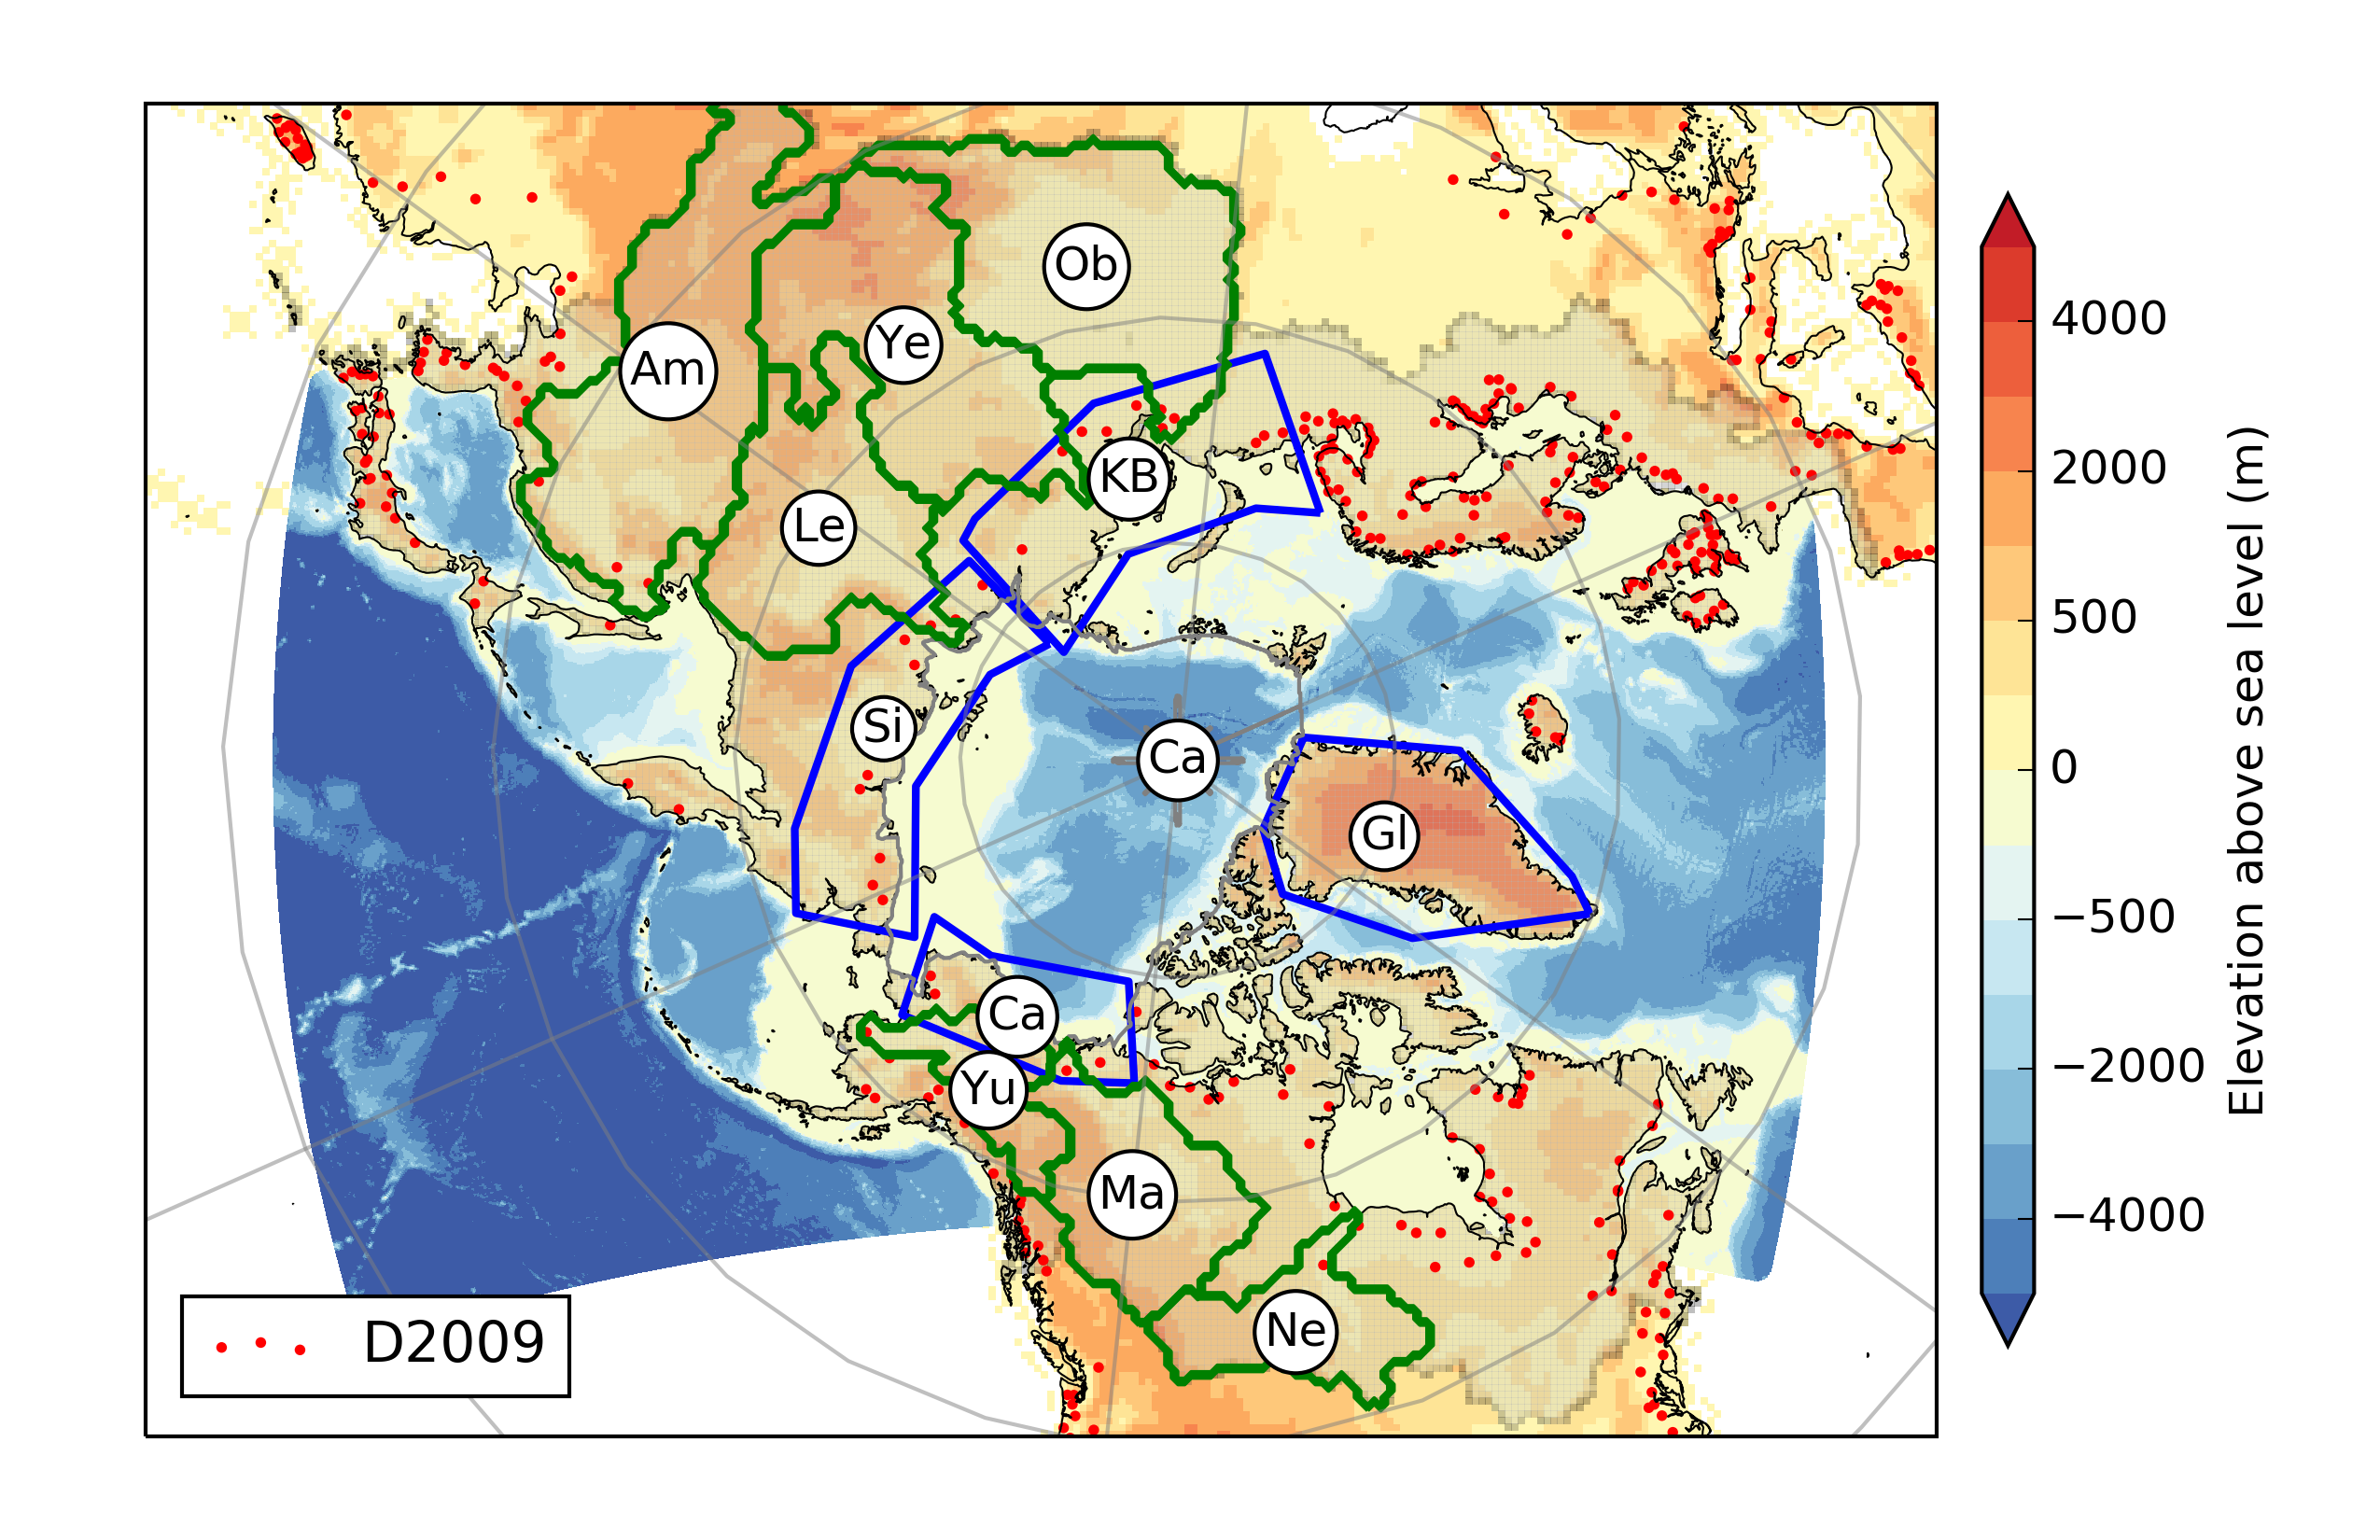
\includegraphics[width=14cm,keepaspectratio]{RASM_domain_fig}
    \caption{The Regional Arctic System Model domain, showing the 50-km near equal area domain shared by the land, atmosphere, and streamflow routing components (outer rectangle), and the 1/12$^\circ$ ocean-sea ice domain (blue shading).
    The RVIC drainage area is highlighted with gray shading and the central Arctic Ocean basin is outlined in gray (Ca).
    The seven largest river basins in the RASM domain are outlined in green: Amur (Am), Ob' (Ob), Yenisey (Ye), Lena (Le), Mackenzie (Ma), Nelson (Ne), and Yukon (Yu).
    The coastal streamflow flux masks used in section \ref{sec:results_ch4} are outlined in blue: Canadian Coast (Ca), Siberian Coast (Si), Kara and Barents Coast (KB), and Greenland (Gl).
    The location of the streamflow observations from $D2009$ are shown with red circles.}
    \label{fig:rasm_domain}
\end{figure}

\subsection{RVIC}
\label{sec:rvic}

% [streamflow routing and other climate models that include coupled land-ocean dynamics]
Most land surface components in ESMs, including the VIC model, do not represent exchanges of moisture between neighboring grid cells, but rely instead on a separate scheme to transport streamflow across the land surface; this process is referred to as streamflow routing.
There are two fundamental approaches to streamflow routing: cell-to-cell (CTC) and source-to-sink (STS).
CTC routing models simulate streamflow by parameterizing the mass flux between neighboring grid cells, explicitly tracking the volume of streamflow between grid cells across the land surface.
CTC routing methods, such as CESM's River Transport Model (RTM) \citep{Branstetter_2003} have been applied globally in a number of GCMs.
Although CTC models are often more physically based than STS models, they have been shown to be difficult to parameterize across a range of spatial scales \citep{Sushama_2004}, limiting their applicability.
STS routing methods \citep[e.g.][]{Lohmann_1996,Naden_1992}, akin to the RVIC model used in this study, do not explicitly track streamflow between grid cells; instead, they parameterize the distribution and travel time of runoff between source and outlet grid points.
In previous applications of STS routing models within coupled GCMs \citep[e.g.][]{Olivera_2000}, the streamflow routing has been applied at coarse spatial resolutions (greater than 200 km) and low-frequency coupling (e.g. daily).

% [Modern day streamflow routing]
New approaches to streamflow routing continue to be developed, adding new routing parameterizations and additional process representations.
Recent examples include MOSART \citep{Li_2013}, CaMa-Flood \citep{Yamazaki_2009,Yamazaki_2014}, and mizuRoute \citep{Clark_2016}.
While a number of routing schemes have been coupled to ESMs \citep[e.g.][]{Sushama_2004,Olivera_2000,Li_2013}, they have rarely been specifically evaluated in terms of coupled land-ocean interactions.
Furthermore, coupled streamflow routing and ocean models have generally not been implemented at a spatial resolution that is sufficient to resolve the coastal currents and streamflow-shelf-basin exchange processes (e.g. eddies) that are particularly important in the Arctic.
In their recent synthesis of the Coupled Model Intercomparison Project \citep[CMIP5; ][]{Taylor_2012} runoff dynamics, \citet{Bring_2015} conclude that a significant community effort is required to improve the understanding and modeling of basin scale freshwater fluxes in coupled climate modeling.
This argument is echoed by \citet{Lique_2015} and \citet{Bring_2016} in their recent review papers on the representation of the Arctic hydrologic cycle in present-day hydrologic and climate models.

The RVIC streamflow routing model is a modified version of the routing model typically used to post-process VIC model output \citep{Lohmann_1996, Lohmann_1998a}.
The original \citet{Lohmann_1996} model has been used in many offline modeling studies from regional to global spatial scales at horizontal resolutions from 1/16$^{\circ}$ to 2$^{\circ}$ \citep[e.g.][]{Nijssen_1997,Lohmann_1998b,Su_2005,Hamlet_2013}.
RVIC is a source-to-sink routing model that solves a linearized version of the Saint-Venant equations \citep{Fread_1992,Mesa_1986}.
The linearized Saint-Venant equations (see Eq. \ref{eq:St_Venant}) are a one-dimensional model describing unsteady flow in terms of two time-invariant parameters, flow velocity and diffusivity.
The velocity and diffusivity parameters can be estimated from observed streamflow or through numeric optimization.
RVIC uses flow direction rasters (FDRs), typically derived from topographic information \citep[e.g.][]{Wu_2011}, to specify the flow path and distance for each source-sink pair.
The flow along the travel path is parameterized as a linear, time-invariant, unit impulse response function (IRF) to runoff generated at individual grid cells by the LSM.
Within hydrology, the IRF is often referred to as a unit hydrograph (UH) \citep[e.g.][]{Sherman_1932,Nash_1957}.
The application of the RVIC model has two distinct steps, a preprocessing step in which IRFs are developed for each source-to-sink pair (see sections ~\ref{sec:irfs} and ~\ref{sec:remap}), and a computationally efficient convolution step in which distributed runoff from the LSM is routed to downstream points (see section~\ref{sec:convolution}).

The RVIC model differs from the original \citet{Lohmann_1996} model in four main ways:

\begin{itemize}
\item RVIC completely separates the development of the IRFs from the flow convolution step,
\item RVIC allows the development of the IRFs to be based on FDR grids that do not match the grid elements used for the LSM (see section~\ref{sec:irfs}),
\item The RVIC convolution scheme operates in a space-before-time pattern, facilitating direct coupling with distributed LSMs (see section~\ref{sec:convolution}),
\item RVIC includes numerous infrastructure software improvements, including parallel processing, the ability to store the exact model state, and to read and write netCDF files.
\end{itemize}

The stand-alone version of the RVIC model, complete with documentation and example input data, is available via a publicly accessible source code repository \citep{Hamman_2015}.

\subsubsection{Impulse response function development}
\label{sec:irfs}

\begin{figure}
    \centering
    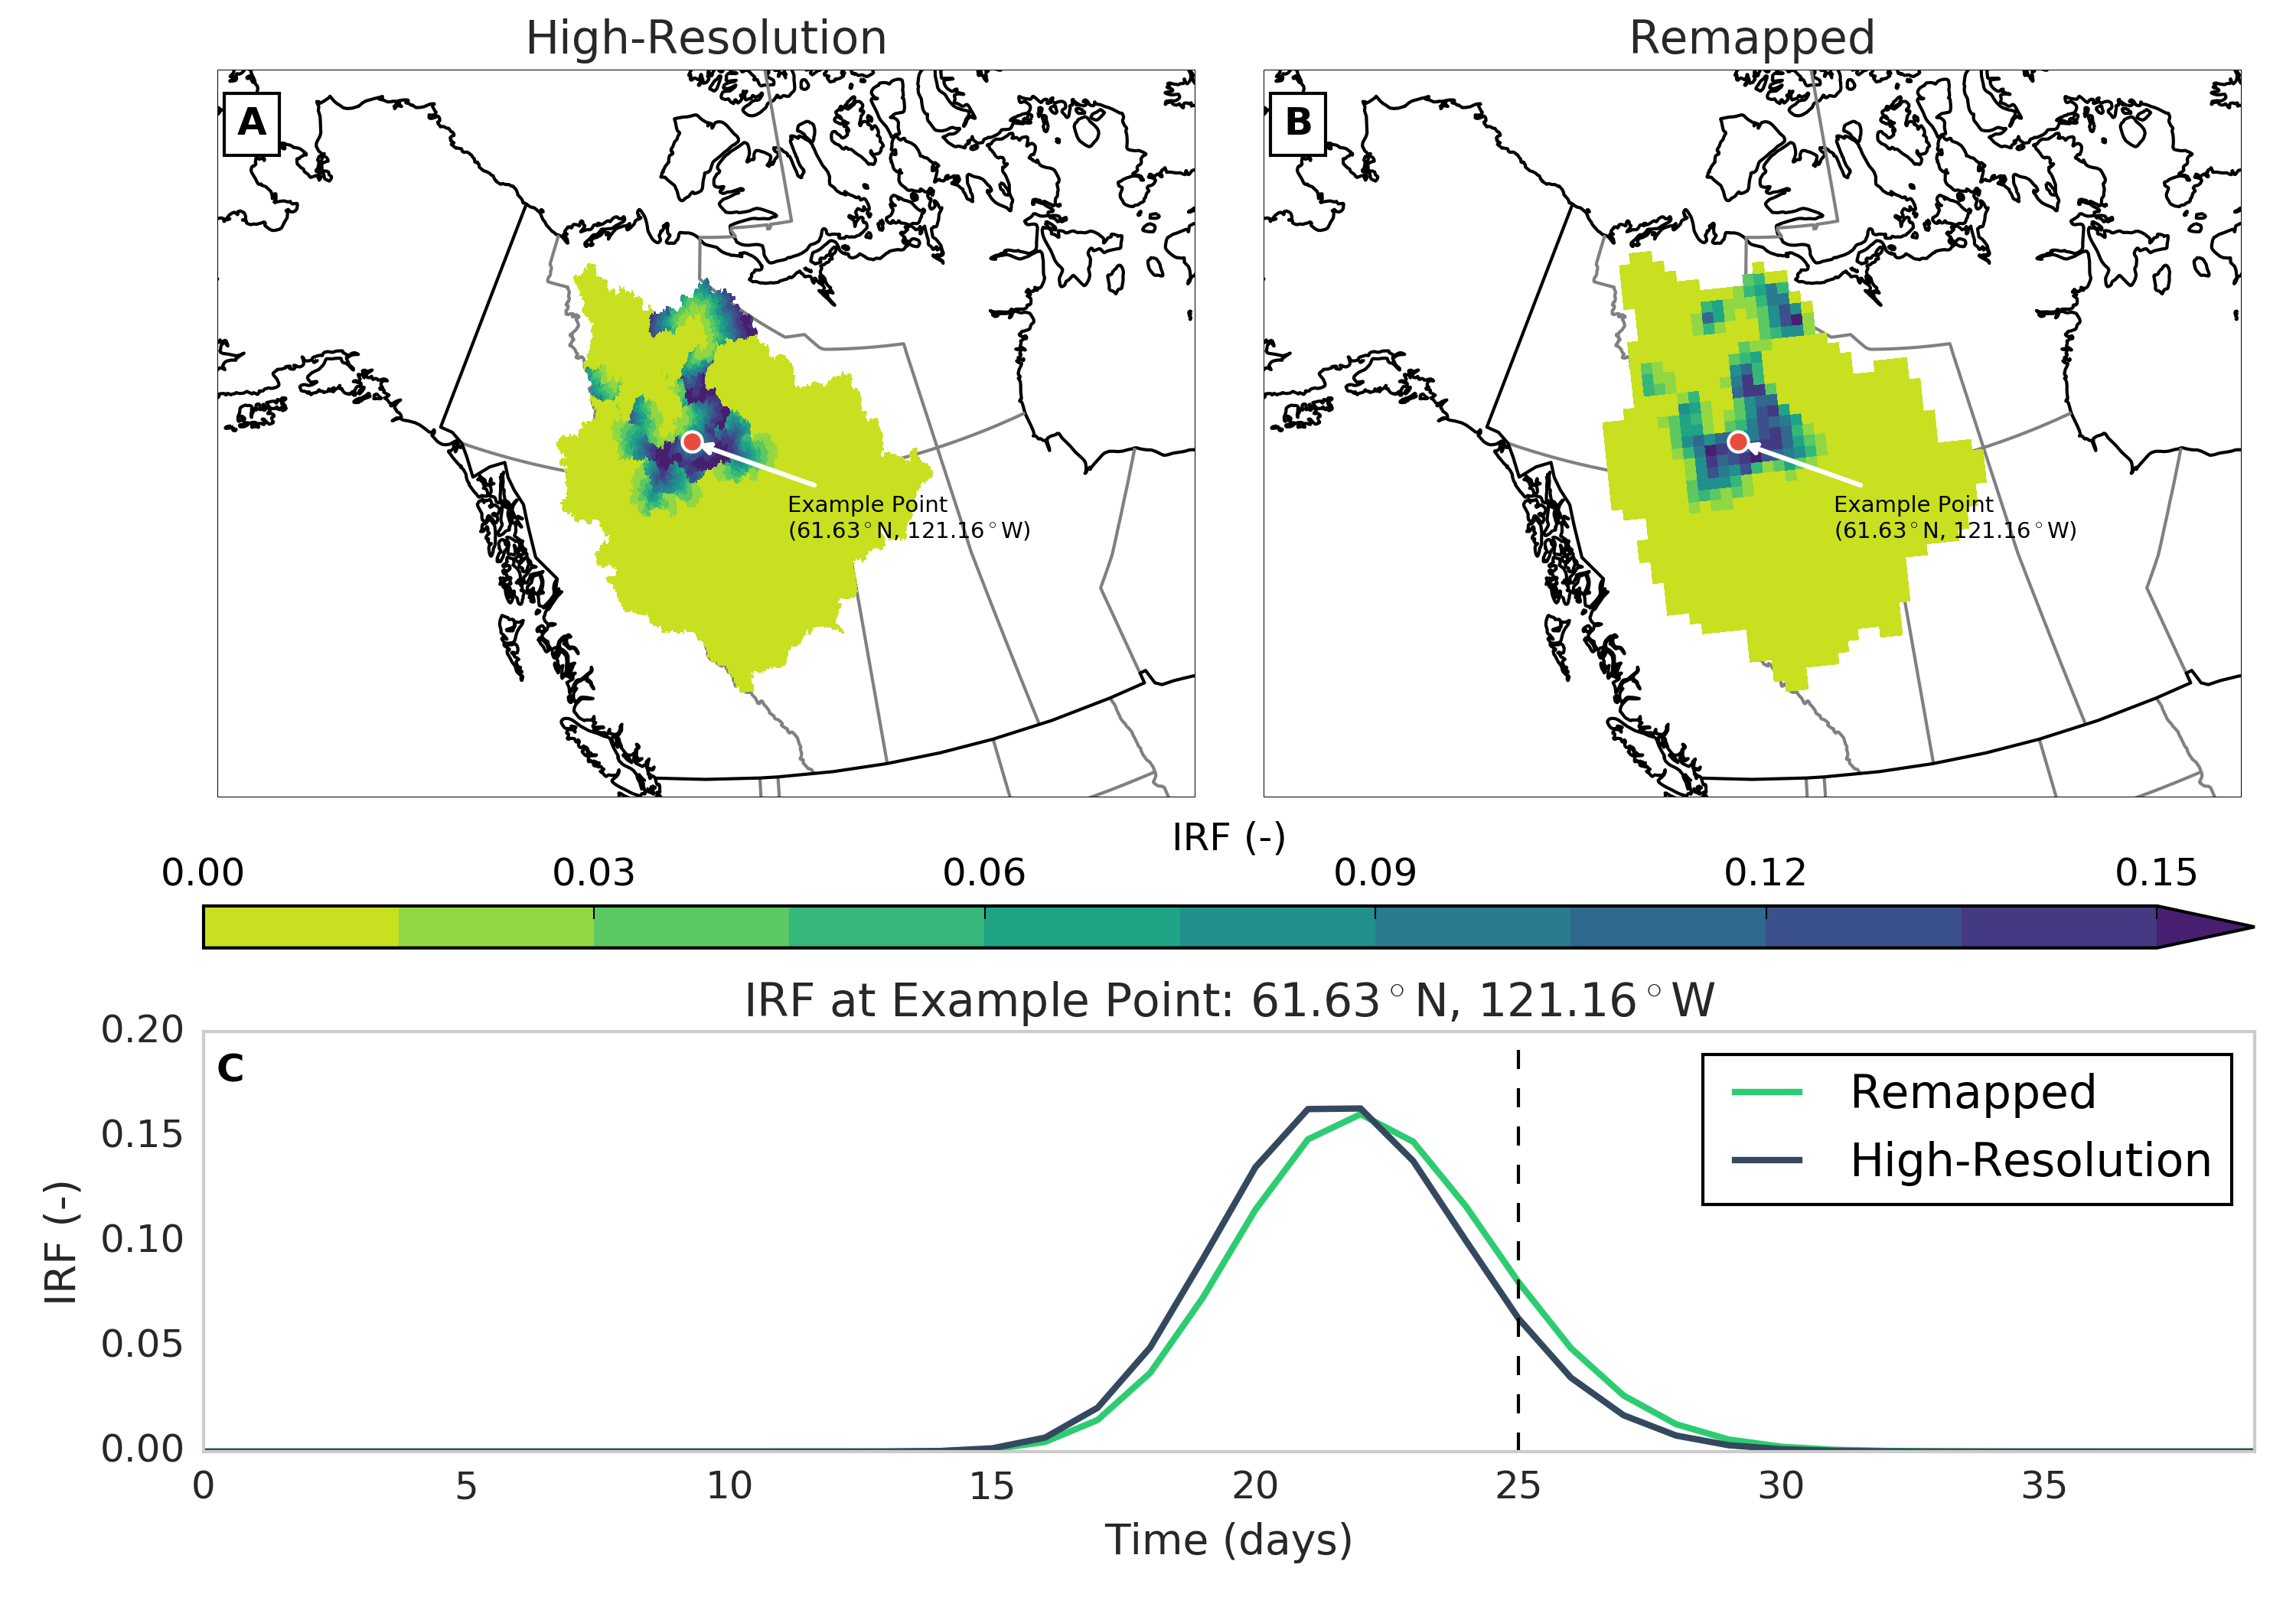
\includegraphics[width=10cm,keepaspectratio]{uh_remap_schematic}
    \caption{Top: High-resolution (A) and remapped (B) IRFs for the Mackenzie River upstream of the Arctic Red River observation location for timestep 25.
    Bottom: IRFs from the high-resolution (blue) and remapped (green) grids at the example location (61.62$^\circ$N, 121.16$^\circ$W) shown in A and B.
    The offset between the two IRFs shown in C is the result of spatial averaging during the remapping step.}
    \label{fig:uh_remap_schematic}
\end{figure}

A UH describes the streamflow response of an area (e.g. basin or grid cell) to a unit input of runoff $Q^F$ in terms of timing and volume (see Figure \ref{fig:uh_remap_schematic}-C).
The IRF for every source-to-sink pair is a combination of an IRF that accounts for flow processes within a grid cell and an IRF that accounts for the horizontal advection-diffusion between the edge of the grid cell and a downstream location.
The horizontal travel path and distance are computed using a flow direction raster \citep[e.g.][]{Wu_2011}.
The Saint-Venant equation is given by

 \begin{equation}
   \label{eq:St_Venant}
   \frac{\partial Q}{\partial t} = D \frac{\partial^2 Q}{\partial x} + C \frac{\partial Q}{\partial x}
 \end{equation}

where $Q$ represents the flow at time $t$ at a downstream point $x$ as a function of the wave velocity $C$ and the diffusivity $D$; both of which may be estimated from geographical data.
Eq.~(\ref{eq:St_Venant}) can be linearized and solved with convolution integrals

 \begin{equation}
   \label{eq:conv_integral}
	  Q(x,t) = \int_0^t UH^{\circ}(t-s)h(x,s)ds
 \end{equation}

where

 \begin{equation}
   \label{eq:Greens_IRF}
	h(x, t) = \frac{x}{2t\sqrt{\pi tD}}exp\left(-\frac{(Ct-x)^2}{4Dt}\right)
 \end{equation}

is a Green's impulse response function, and $UH^{\circ}$ is the IRF (or unit hydrograph) that accounts for flow processes within each source grid cell.
Equations \ref{eq:conv_integral} and \ref{eq:Greens_IRF} are solved to determine the flow response for each source-to-sink pair.

\subsubsection{Upscaling and basin aggregation}
\label{sec:remap}

The original implementation of the \citet{Lohmann_1996} model required an exact match between the FDR grid and the LSM grid.
This limited the applicability of the model and required either for the LSM to be implemented on the same grid as an existing FDR or the custom generation of an FDR for each LSM grid.
The RVIC implementation allows for the derivation of the IRFs on an arbitrary grid and a subsequent remapping of the IRFs unto the LSM grid.
As a consequence, IRFs can be calculated once based on a high-resolution FDR grid and subsequently upscaled and aggregated to different LSM grids (Figure \ref{fig:uh_remap_schematic}).
The upscaling process spatially remaps the IRFs from the high-resolution FDR grid to the LSM grid using the first-order conservative remapping technique developed by \citet{Jones_1999}.
Because the remapping scheme is conservative, each of the resulting IRFs on the LSM grid is an area-weighted average of the IRFs on the high-resolution FDR grid.
Finally, in the event there are multiple sink points on the FDR grid within a single LSM grid cell, the upscaled IRFs are combined to include all source points flowing into a single outlet grid cell.

\subsubsection{Convolution}
\label{sec:convolution}

The convolution step combines the IRFs with the discharge fluxes from the LSM.
The streamflow $Q$ for each outlet grid cell $x$ and time step $t$ is given by

\begin{equation}
  \label{eq:convolution}
   Q(x,t) = \int_0^{S(x)} \int_0^{\infty}\,IRF(s,t)\,Q^F(s,t-\tau)\,d\tau\,ds
 \end{equation}

where $S(x)$ is the number of source grid cells upstream of each outlet ($x$), and $\tau$ is the position in the IRF vector.
RVIC's application of the convolution is practically equivalent to the one described by \citet{Lohmann_1996}.
The key difference is in the implementation, where the time integral has been moved to the outer loop in RVIC, allowing for stepwise evaluation of the convolution over the entire spatial model domain.

\subsubsection{RVIC in RASM}

The IRFs used in RASM were developed using the 1/16$^{\circ}$ FDRs from \citet{Wu_2011}.
RVIC in RASM uses a spatially constant flow velocity and diffusivity of 0.6 m/s and 3,000 m$^2$/s, respectively.
These parameters were chosen using the calibration methods described in section~\ref{sec:parameters}.
Hourly IRFs were developed for each of the 95,001 coastal 1/16$^{\circ}$ grid cells bordering the ocean model and were upscaled and aggregated to the 4,841 coastal grid cells on the 50-km near equal area land surface grid that is used by RASM version 1.0.

In nature, turbulent mixing and other diffusive processes combine to gradually spread fresh water along the coast and into the open ocean.
In a coupled modeling environment, however, these processes are difficult to represent at the spatial scales at which the runoff, ocean, and sea ice models are configured.
To simulate the dispersion of fresh water throughout each ocean grid cell within RASM, a diffusion scheme is applied within the coupler (CPL7) to avoid unrealistic salinity gradients that could occur where a river's entire outflow is applied to a single ocean grid cell.
The mapping from the runoff grid to the ocean grid is generated as a preprocessing step using the masks and geometries of the runoff and ocean grids.
Each runoff grid cell is mapped to the nearest ocean grid cell.
The flux is then smoothed over all grid cells in a 300 km radius $r_{max}$ with a distance $r$ weighted logarithmically decreasing e-folding scale $r_{fold}$ of 1000 km such that the total runoff flux to the ocean is conserved.
These parameters were chosen to minimize smoothing while ensuring that negative salinities were not encountered along the coast.

The mapping weights $w(r)$ are given by

\begin{equation}
  \label{eq:diffusion}
  w(r)=
     \begin{cases}
        e^{(-r/r_{fold})} 0\leq r\leq r_{max} \\
        0 r > r_{max}
     \end{cases}
\end{equation}

\subsection{Parameter Selection}
\label{sec:parameters}

The commonly used ``default'' velocity and diffusivity parameters for the \citet{Lohmann_1996} and RVIC models are 2.0 m/s and 2,000 m\textsuperscript{2}/s, respectively.
Early RASM simulations, however, indicated that there was a large timing bias in the RVIC model, indicating that the default parameter values were not adequately describing the routing behavior in the Arctic.
To correct this timing bias, we applied a simple, brute force parameter evaluation procedure to select the velocity and diffusivity parameters that best described the routing behavior in the Arctic drainage basin.
For this procedure, RVIC was run offline (i.e. not coupled to RASM) at a daily timestep and was forced using daily runoff fluxes from the fully-coupled RASM simulation described as $RASM_{ERA}$ in \citet{Hamman_2016a}.
These runoff fluxes include both the fast-response and slow-response runoff components generated by the LSM.
The velocity and diffusivity parameters were varied between 0.2-1.5 m/s and 500-4,000 m\textsuperscript{2}/s respectively; ranges consistent with the the plausible values discussed in the relevant literature \citep[e.g.][]{Decharme_2010,Lohmann_1996}.
Individual pairs of parameters were evaluated using a modified version of the overlap statistic \citep{Perkins_2007} as the objective function.
The overlap statistic, which was originally introduced as a measure of likeness for probability density functions, is applied here to the normalized mean monthly hydrographs of the six largest river basins in the RASM model domain (Figure \ref{fig:rasm_domain}).
The overlap statistic based on normalized flows is perhaps the most appropriate performance measure of the routing model because it focuses entirely on the shape of the hydrograph and does not take the bias in the annual flow volume into account (Figure \ref{fig:calibration_hydrographs}).
This is desirable since the volume bias is determined by the LSM (and the other components in the coupled model) and is not affected by the routing model, which is mass-conserving.
The final velocity and diffusivity parameters, 0.6 m/s and 3,000 m\textsuperscript{2}/s, respectively, were chosen to maximize the composite overlap statistic for the six largest rivers in the RASM domain, where the composite was formed by weighting each basin's overlap statistic by that basin's annual runoff volume.

\begin{figure}
    \centering
    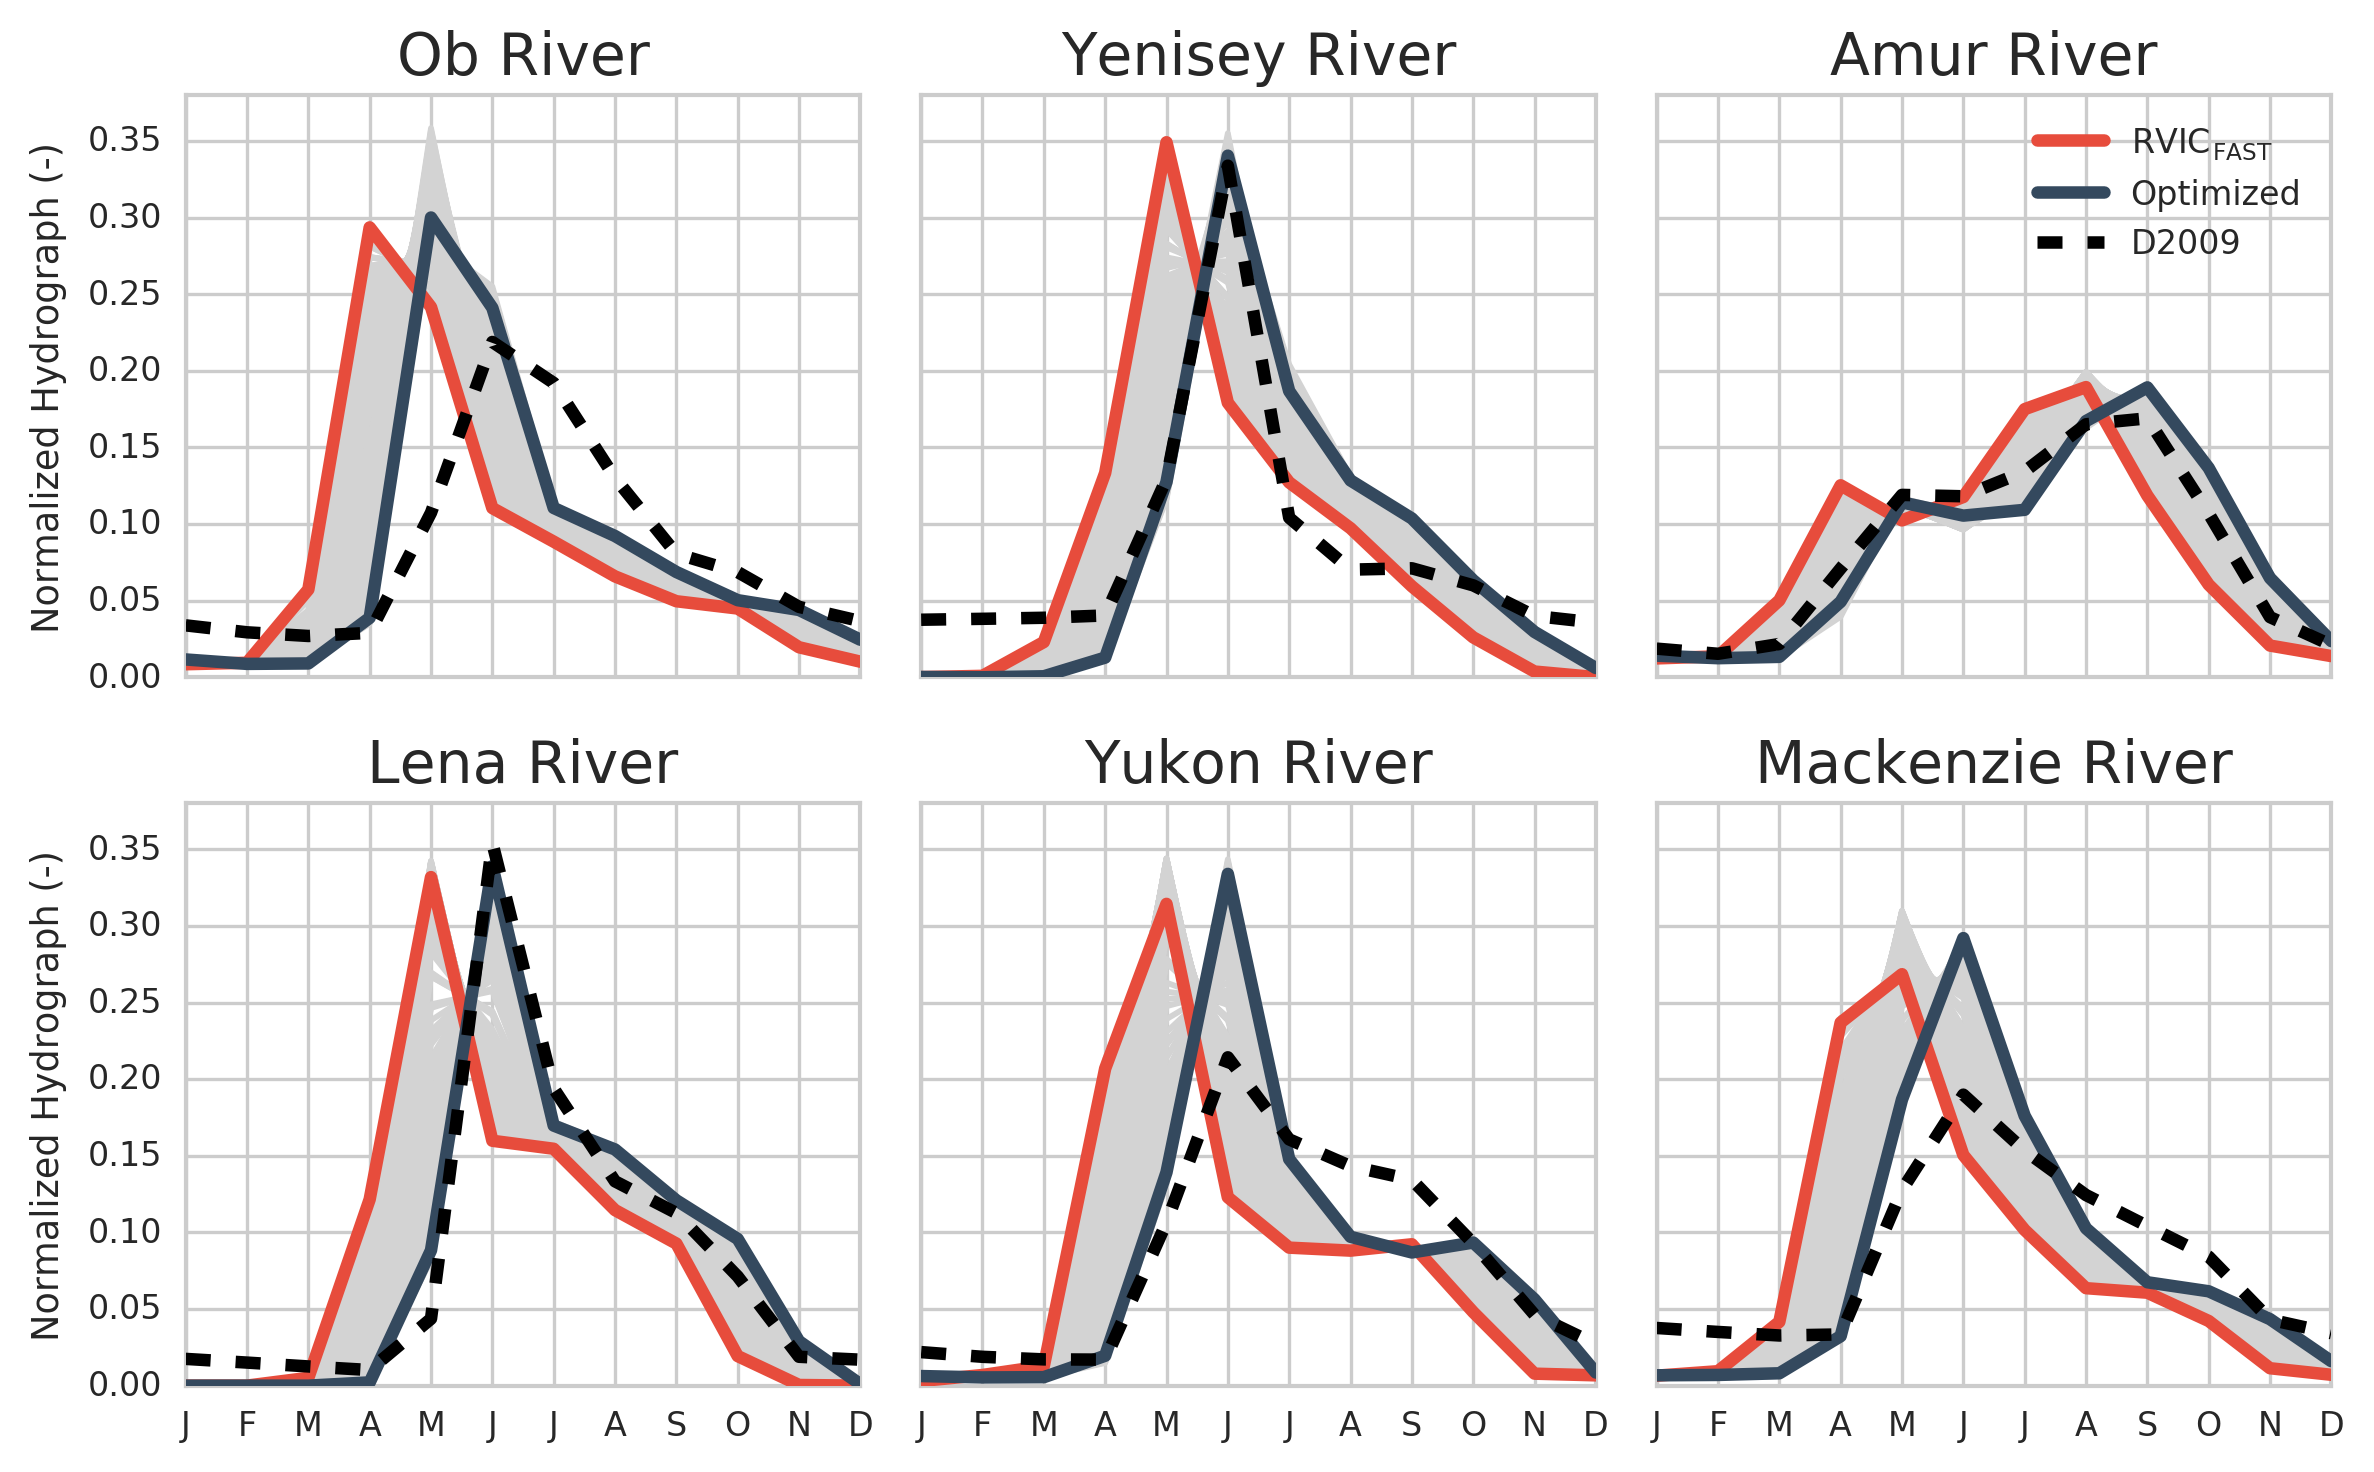
\includegraphics[width=10cm,keepaspectratio]{calibration_hydrographs}
    \caption{Normalized annual hydrographs for largest six river basins in the RASM domain.
    Each trace (grey) represents an individual calibration ensemble member.
    The hydrographs using the optimized parameters are shown with blue lines.
    The normalized observed hydrograph from $D2009$ for each basin is shown with the dashed black line and the hydrograph using the $RVIC_{FAST}$ (default) parameters is shown with the red line.}
    \label{fig:calibration_hydrographs}
\end{figure}

\section{Model Simulations and Data}
\label{sec:data_ch4}

We present results from two fully-coupled RASM simulations, the baseline ($RASM_{CONTROL}$) and a modified simulation (without the streamflow flux; $RASM_{NOROF}$), using RASM version 1.0, each using ERA-Interim boundary conditions (Table \ref{table:simulations}).
In addition, to highlight the impact of the calibration procedure we include results from an offline RVIC simulation, $RVIC_{FAST}$, forced with VIC discharge from $RASM_{CONTROL}$.
All three simulations were run from September 1, 1979 through December 31, 2014.
For the RASM simulations, we focus our analysis on the period January 1, 1990 through December 31, 2009, allowing for a 10-year model spin-up of the coupled system.
Both RASM simulations began with the same initial state \citep[see ][]{Hamman_2016a} and use identical land, atmosphere, ocean, and sea ice model configurations.
POP was initialized from a no-motion state with climatological temperature and salinity fields derived from the University of Washington Polar Science Center Hydrographic Climatology version 3.0 \citep{Steele_2001}.
The 75-year ice-ocean spin-up consisted of an initial integration starting from 1948 through 1992 followed by a second integration from 1948 through 1979, both forced with $CORE.v2$ (see below).

\begin{table}[]
  \caption{Summary of model simulations.}
  \label{table:simulations}
  \begin{tabular}{l|p{4in}}
  Simulation       & Description \\
  $RASM_{CONTROL}$ & Baseline simulation, uses the calibrated RVIC parameters described in section \ref{sec:parameters}. \\
  $RASM_{NOROF}$   & Same as $RASM_{CONTROL}$ except does not include the runoff flux from the land to the ocean. \\
  $RVIC_{FAST}$    & Stand-alone RVIC simulation forced with distributed runoff fields from $RASM_{CONTROL}$. This simulation uses RVIC's default velocity and diffusivity parameters of 2.0 m/s and 2,000 m\textsuperscript\{2\}/s, respectively.
  \end{tabular}
\end{table}

We compare our model simulated streamflow to in-situ streamflow observations in the \citet{Dai_2009} dataset, hereafter referred to as $D2009$.
This dataset provides mean monthly streamflow observations at the most downstream gauging location for more than 50 individual river basins within the RASM domain and analysis period.
Temporal gaps in the observed data record were filled by \citet{Dai_2009} using a combination of linear regression and model derived streamflow fluxes (from the Community Land Model, version 3), forced with observed meteorology.
In section \ref{sec:discussion_ch4}, we also compare the RASM coastal streamflow flux to $CORE.v2$ \citep{Large_2009} and the combined Greenland freshwater discharge estimates from $Bamber_{GR}$ \citep{Bamber_2012}.
The $CORE.v2$ runoff data was also constructed by \citet{Dai_2009} using the same observations as in $D2009$.
$CORE.v2$ was further blended with model estimates to fill in ungauged areas and was adjusted to close the global water budget and is frequently used as a forcing dataset for global and regional ocean modeling.
$CORE.v2$ is available at a monthly timestep and a 1$^{\circ}$ grid resolution.
We also use data from the high-resolution (11 km) regional atmospheric climate model (RACMO2) applied over Greenland, hereafter referred to as $Bamber_{GR}$.
This dataset provides the best-known freshwater discharge estimates for Greenland and is comprised of monthly means for the runoff and solid ice flux for the period 1958-2010.

\section{Results}
\label{sec:results_ch4}

\subsection{Modeled vs. Observed Streamflow}
\label{sec:hydrographs}

Our analysis of the RASM streamflow flux extends the results of \citet{Hamman_2016a} from the annual to the monthly timestep.
Figure \ref{fig:hydrographs} compares the monthly hydrographs for $RVIC_{FAST}$ and $RASM_{CONTROL}$ simulations at seven of the streamflow gauge locations shown in Figure \ref{fig:rasm_domain}.
These hydrographs are compared to $D2009$ for the period 1990 to 2006.
The annual overlap and monthly RMSE statistics for these seven basins are shown in Table \ref{table:rivers}.
The peak spring freshet in $RVIC_{FAST}$ occurs one to two months earlier than $D2009$ and typically one month earlier than in $RASM_{CONTROL}$.
On average, this leads to normalized overlap statistics in $RVIC_{FAST}$ that are about 15\% lower than for the $RASM_{CONTROL}$ simulation.
The differences in the routing parameters used in the $RVIC_{FAST}$ and $RASM_{CONTROL}$ simulations can be clearly identified in the annual cycle column of Figure \ref{fig:hydrographs}.
The earlier spring freshet in $RVIC_{FAST}$ compared to $RASM_{CONTROL}$ is mostly due to the difference in streamflow velocity (2.0 vs. 0.6 m/s), whereas the shape of the hydrograph is largely determined by the diffusivity parameter (2,000 vs. 6,000 m\textsuperscript{2}/s).

\begin{table}
  \caption{RVIC model performance statistics for the seven rivers shown in Figure \ref{fig:rasm_domain}. The overlap statistic is calculated using normalized hydrographs whereas the bias and RMSE are calculated using the unadjusted hydrographs.}
  \label{table:rivers}
  \resizebox{\textwidth}{!}{%
  \begin{tabular}{|l|c|c|c|c|c|c|}
  {} & \multicolumn{1}{c}{Bias (\%)} & \multicolumn{2}{c}{Overlap (-)}  &  \multicolumn{2}{c}{RMSE (100 $m^3/s$)} \\
  River                   & $RASM_{CONTROL}$ & $RVIC_{FAST}$ & $RASM_{CONTROL}$ & $RVIC_{FAST}$ & $RASM_{CONTROL}$ \\
  Ob' at Salekhard         &            -3.9  &          0.65 &             0.73 &      148.7    &         120.9    \\
  Yenisey at Igarka       &           -25.8  &          0.64 &             0.75 &      201.1    &         137.9    \\
  Amur at Komsomolsk      &            26.9  &          0.93 &             0.90 &       67.1    &          68.3    \\
  Lena at Kusur           &           -28.0  &          0.64 &             0.80 &      207.3    &         137.1    \\
  Yukon at Pilot          &            13.2  &          0.66 &             0.79 &       73.6    &          50.9    \\
  Mackenzie at Arctic Red &            -4.0  &          0.67 &             0.75 &       82.2    &          62.2    \\
  Nelson at Bladder       &            61.3  &          0.70 &             0.71 &       29.2    &          28.8    \\
  \end{tabular}
}
\end{table}

The improved performance of RVIC in $RASM_{CONTROL}$, relative to $RVIC_{FAST}$, highlights the impact of parameter selection and demonstrates the improvement that can be achieved through a relatively simple parameter optimization.
It also shows the limits of the RVIC model, which is mass-conserving.
Compared to the normalized hydrographs in Figure \ref{fig:calibration_hydrographs}, most of the disagreement in Figure \ref{fig:hydrographs} is due to the bias in the total annual runoff flux.
\citet{Hamman_2016a} provided a more detailed, intermodel comparison of the annual runoff biases in the Arctic and found that the performance of VIC in RASM is as good or better than a number of other coupled land-atmosphere models.

The $RASM_{CONTROL}$ hydrographs in the Amur, Lena, and Yukon Rivers match $D2009$ best, with normalized overlap statistics between 0.79 and 0.9.
In the Ob, Yenisey, and Mackenzie River basins, the $RASM_{CONTROL}$ streamflow shows positive biases in the winter and spring and negative biases in the summer.
Consequently, the overlap statistic for these rivers is lower ($<$ 0.75).
VIC underestimates the baseflow flux in these basins, particularly during the winter.
Biases in the winter baseflow flux have previously been identified in VIC and other LSMs applied in the Arctic \citep{Slater_2007}.
For most of the basins shown in Figure \ref{fig:hydrographs}, the timing of the spring freshet in the $RASM_{CONTROL}$ simulation occurs one month before $D2009$.
This timing bias likely results from a spring and summer warm bias in the $RASM_{CONTROL}$ simulation \citep{Hamman_2016a,Cassano_2016}, resulting in premature snowmelt and runoff.
Evidence for this can be found by comparing the timing of the peak streamflow in Figures \ref{fig:calibration_hydrographs} and \ref{fig:hydrographs}.
Whereas the RASM simulations used for the calibration procedure had relatively small spring season temperature and snowmelt timing biases \citep{Hamman_2016a}, the RASM simulations used here include a premature snowmelt leading to timing biases in the spring freshet.
The one exception to this explanation is the Ob' River basin, where the spring peak occurs a month early in both the calibrated and $RASM_{CONTROL}$ (May vs. June).
We attribute these timing biases in the Ob' River basin to the influence of the extensive wetlands and permafrost, processes that affect streamflow behavior which RVIC is not accurately capturing.
Note that for the RVIC setups used in this paper, the velocity and diffusivity parameters were kept constant over the entire domain.
Basin-specific parameters may improve the representation of regional variations in streamflow dynamics, such as the timing of the spring peak in the Ob' basin.

\begin{figure}
    \centering
    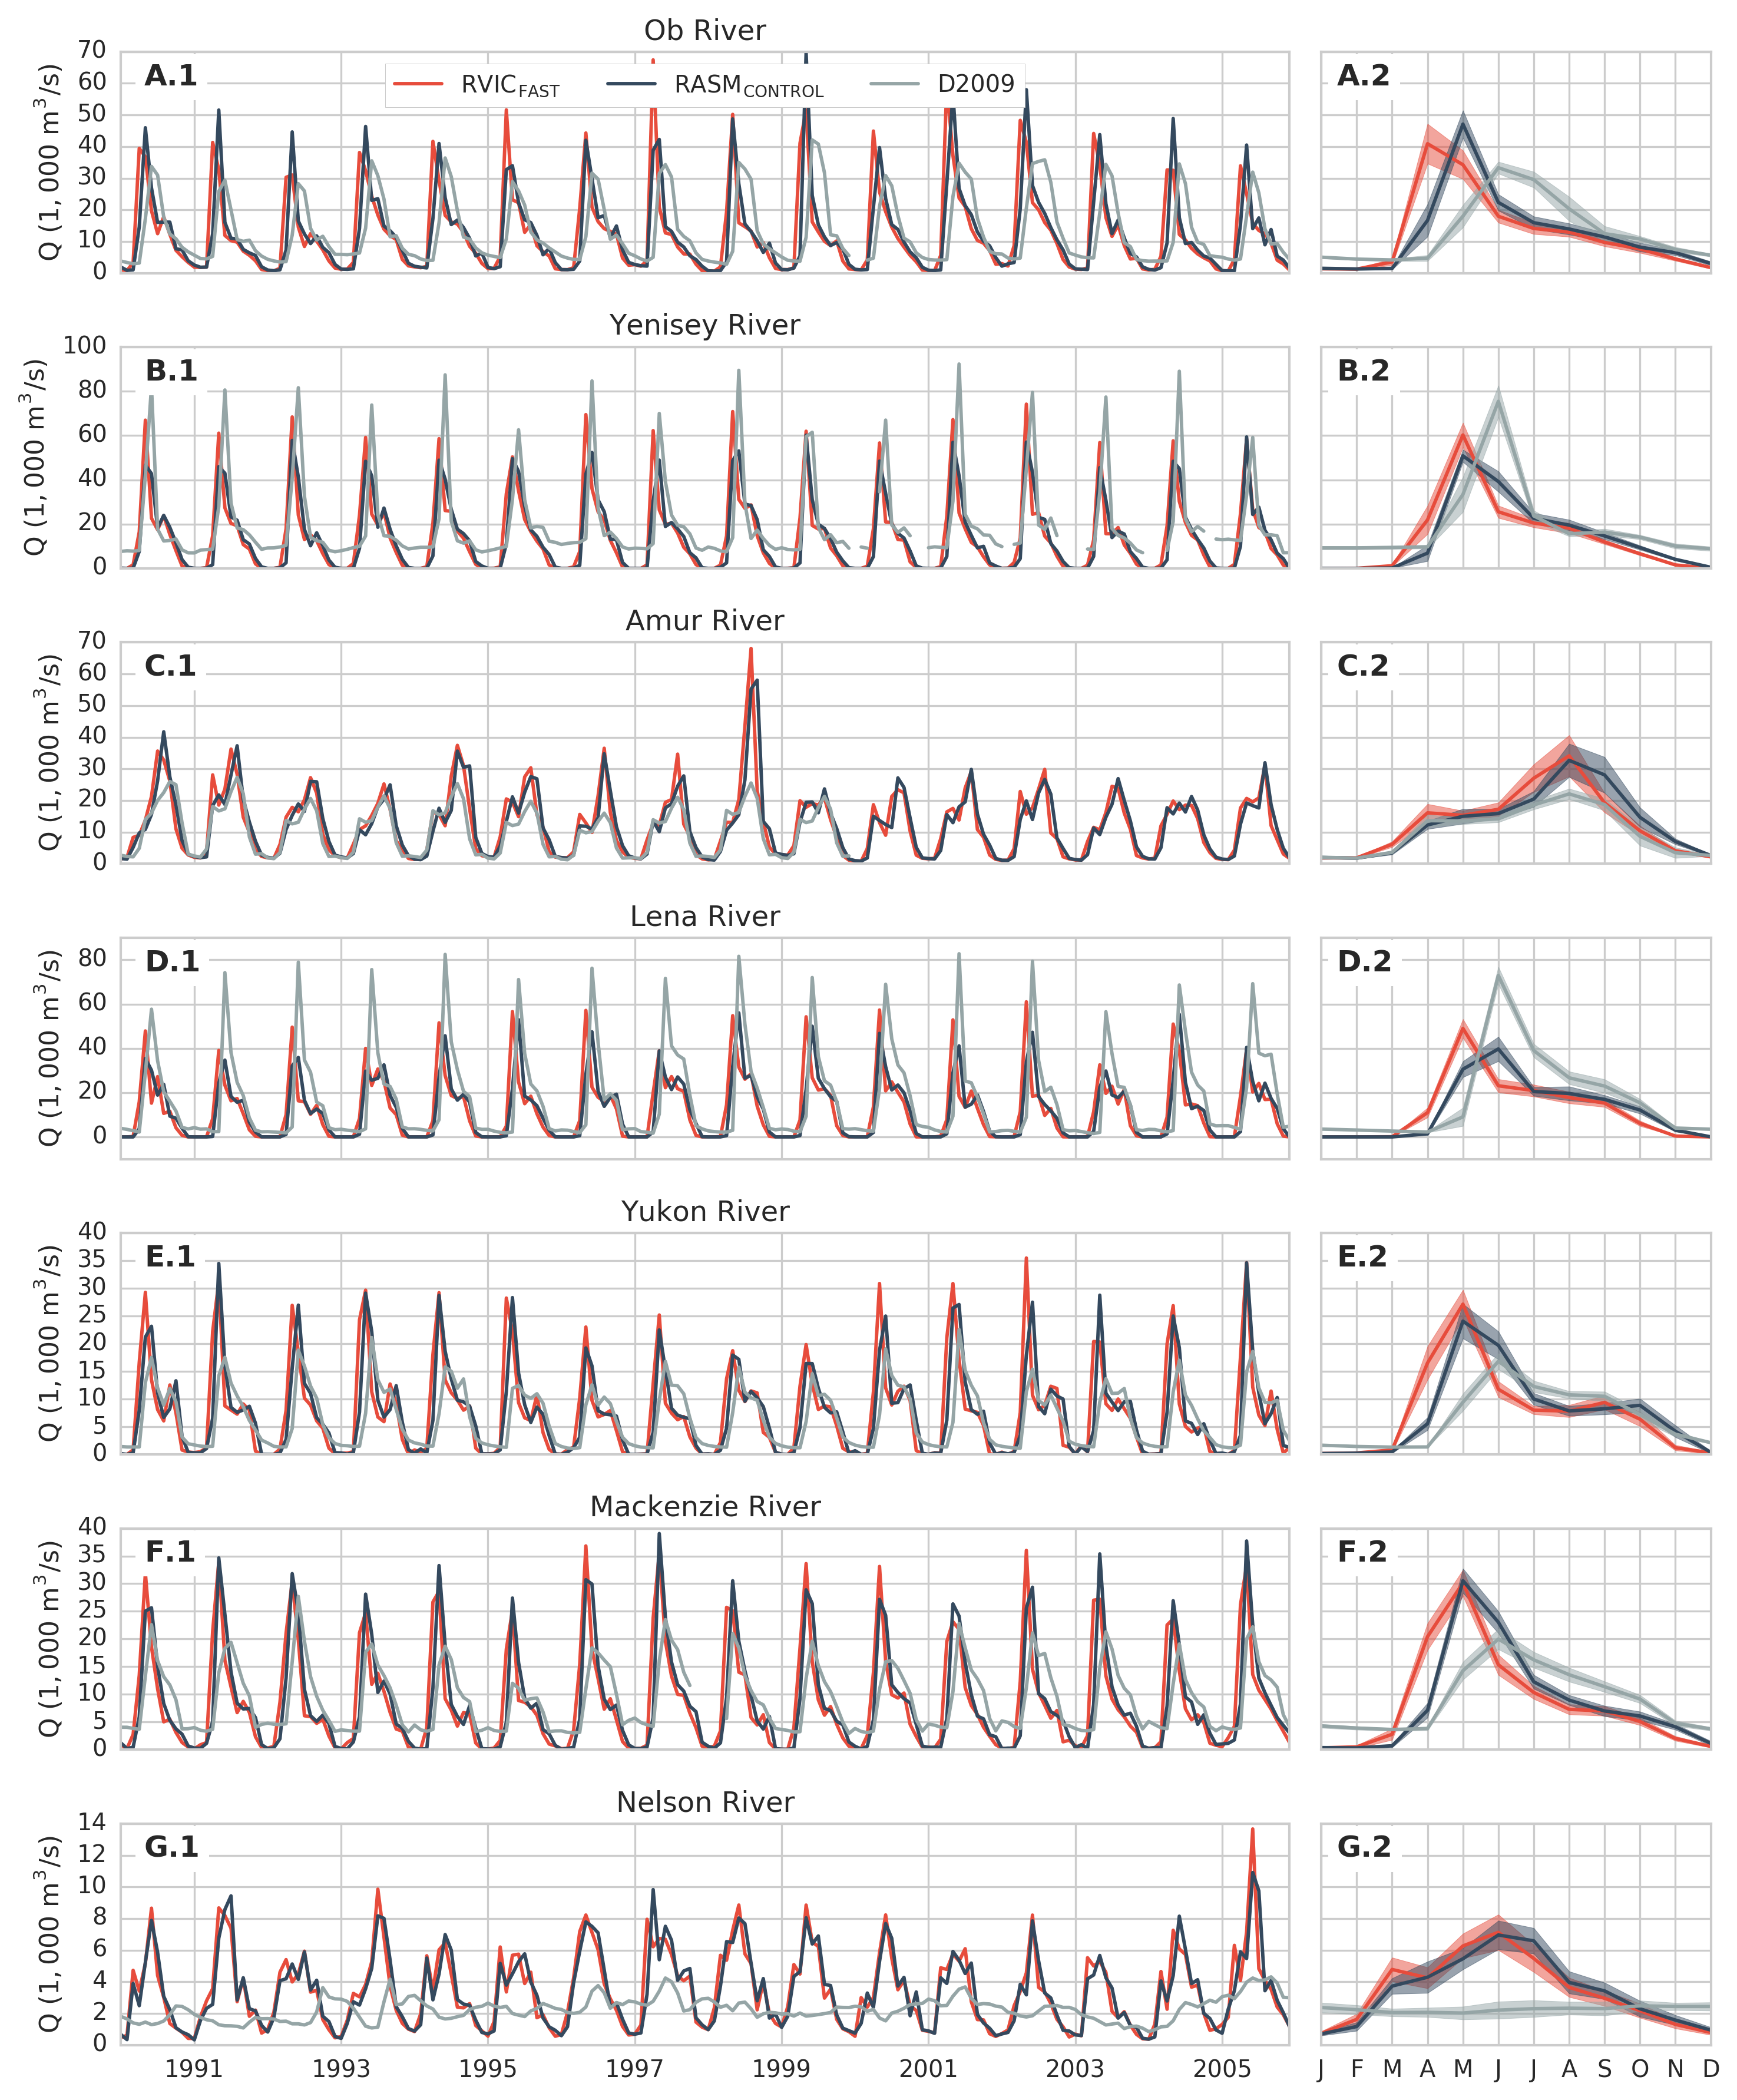
\includegraphics[width=15cm,keepaspectratio]{R1010RBRbaaa01a_rvicfast_hydrographs}
    \caption{Streamflow hydrographs from $RASM_{CONTROL}$ (blue) and $RVIC_{FAST}$ (red) for the largest seven river basins compared to values from $D2009$ (gray).
    The left column includes the monthly streamflow timeseries and the right column includes the monthly mean annual hydrograph where the standard deviation of the interannual variability is represented by the shading.}
    \label{fig:hydrographs}
\end{figure}

Figure \ref{fig:taylor} shows a Taylor diagram comparing the RASM simulated monthly hydrographs at 51 observation locations within the RASM domain.
The Taylor diagram shows the correlation along the arc and the normalized standard deviation ratio along the radius.
The contours denote lines of equal root-mean-square error (RMSE) where a correlation of 1.0 and a standard deviation ratio of 1.0 reflects an RMSE of zero.
In general, moving down on the Taylor diagram indicates improved model skill.
The largest basins in $RASM_{CONTROL}$ tend to perform better with correlation coefficients typically increasing by about 0.3, relative to $RVIC_{FAST}$.
This comes by design, since the performance for those basins was optimized during calibration.
While the correlations are shown to improve in nearly all of the basins in Figure \ref{fig:taylor}, the standard deviations are not significantly impacted by the calibration.
This indicates that the variability in the monthly time series is not significantly controlled by the routing model and is more a function of the runoff flux coming from the LSM.

\begin{figure}
    \centering
    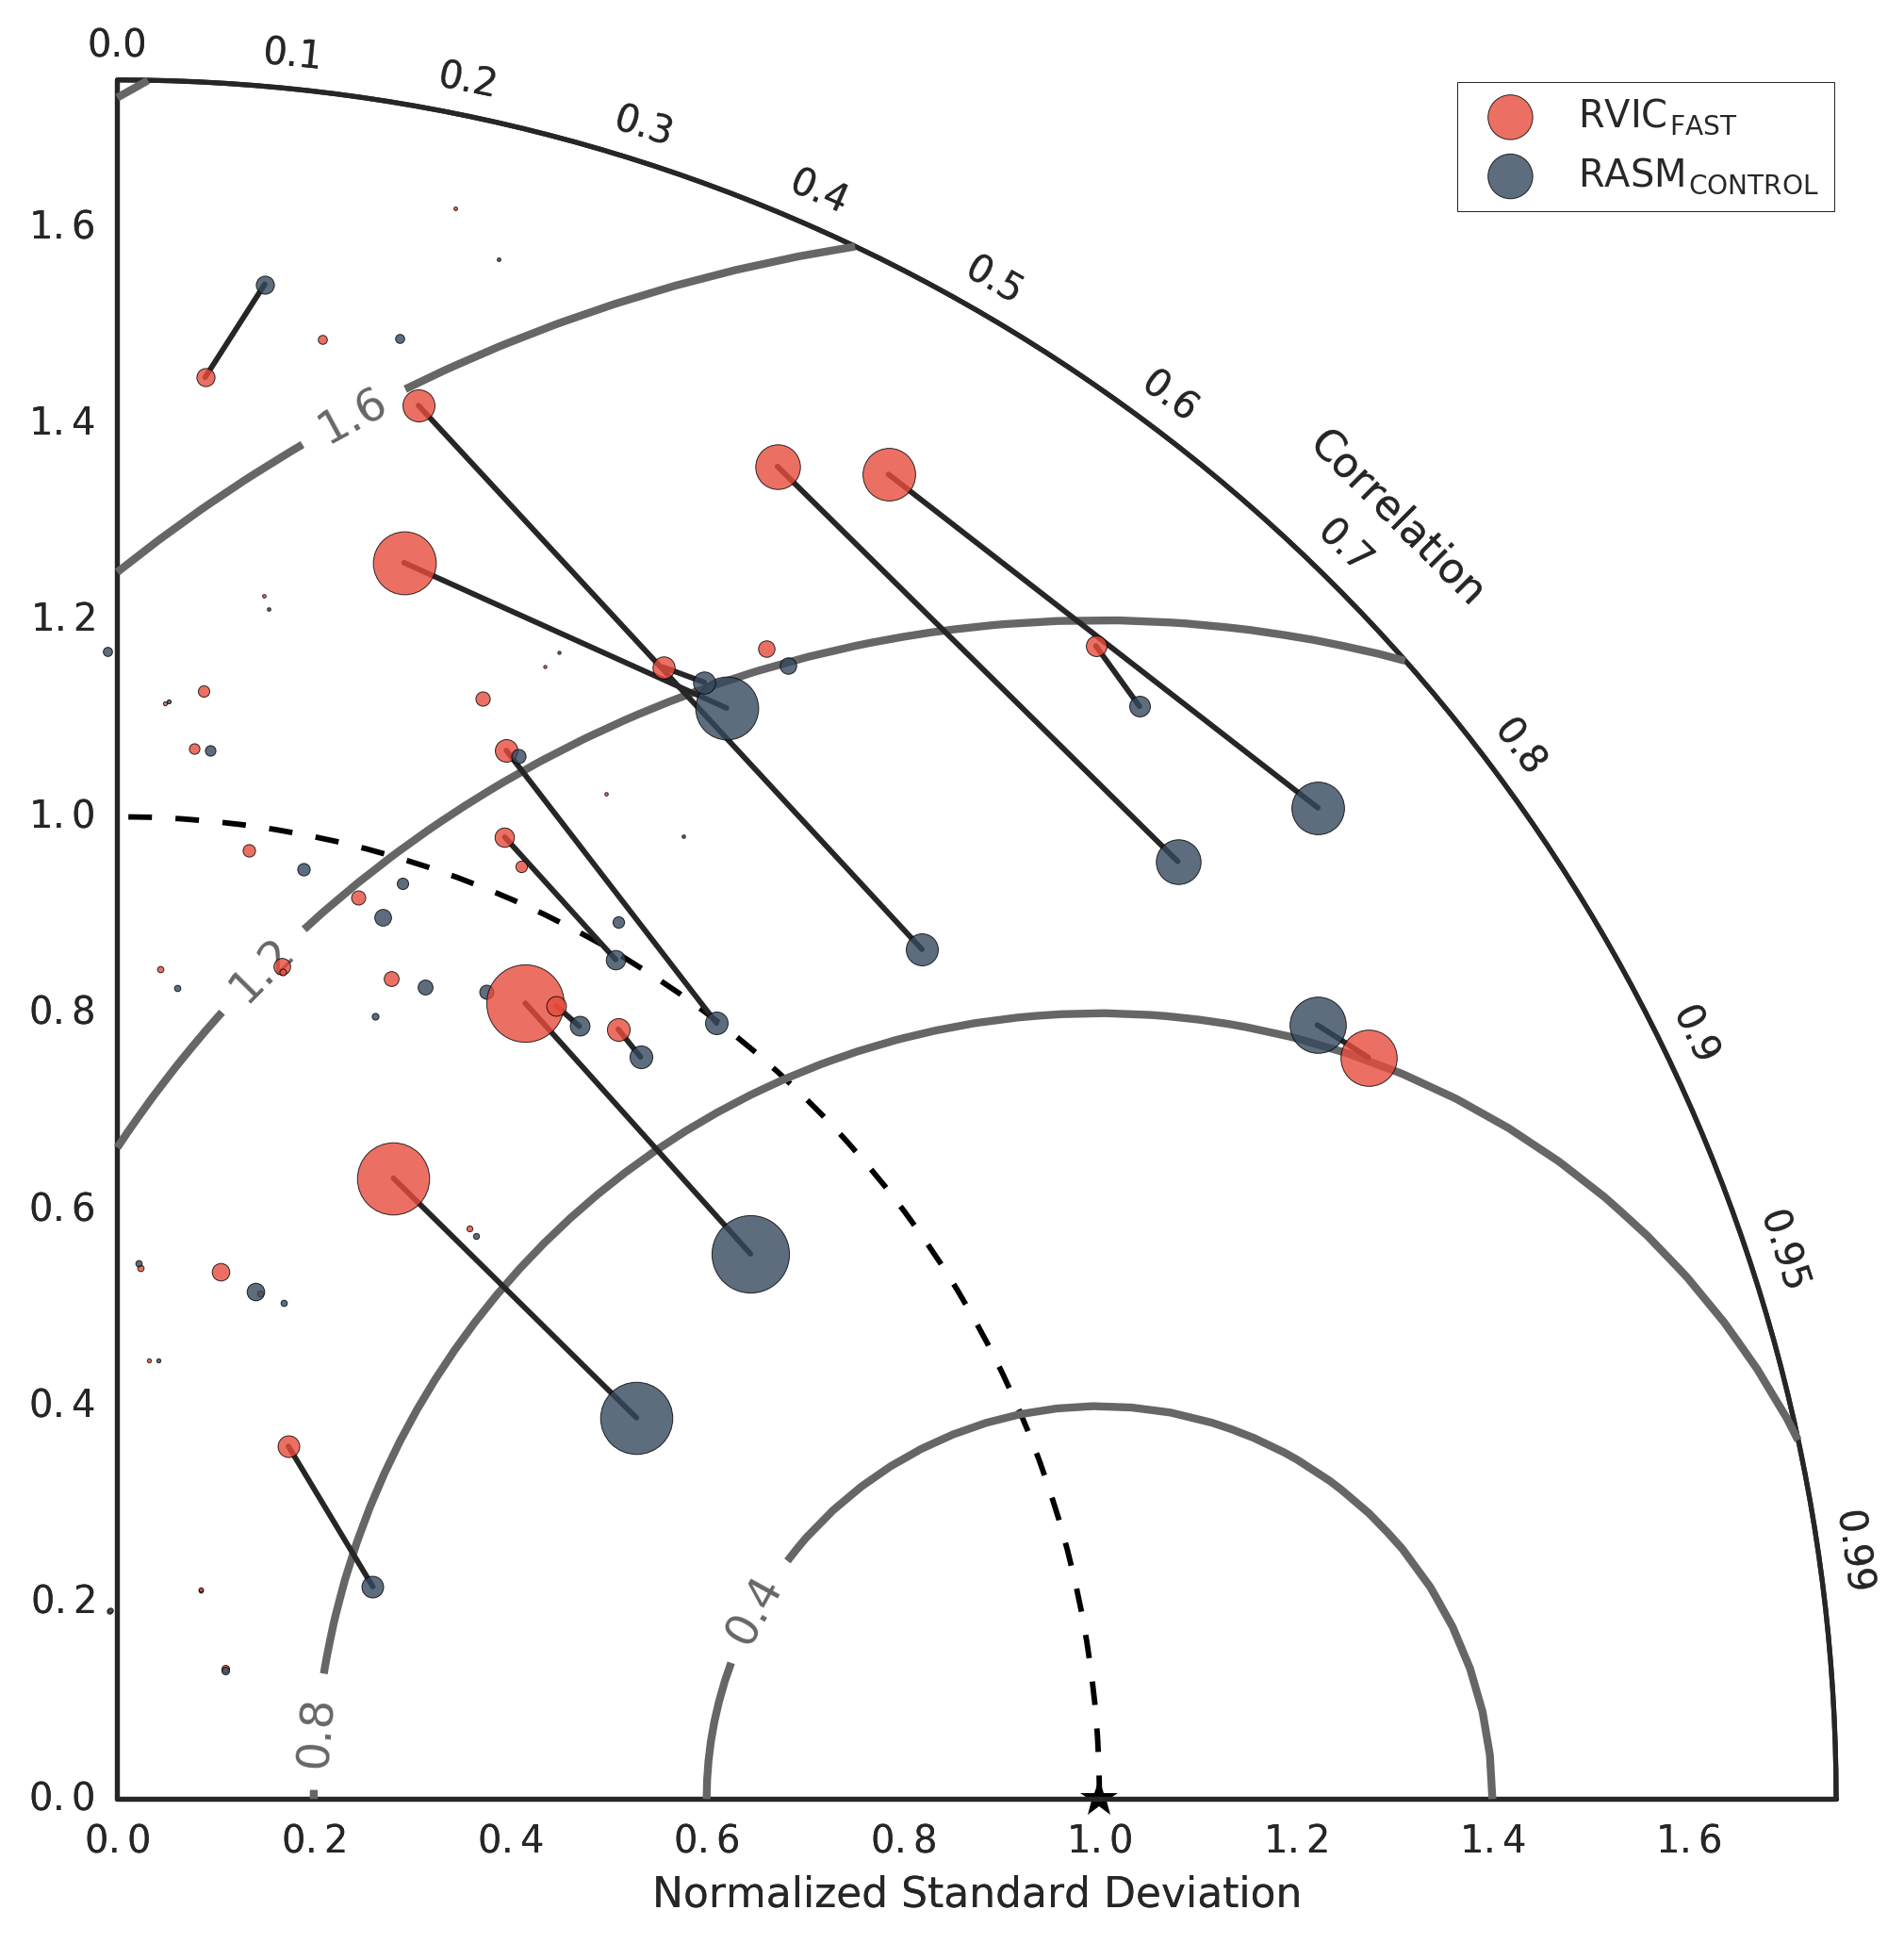
\includegraphics[width=10cm,keepaspectratio]{R1010RBRbaaa01a_rvicfast_taylordiag}
    \caption{Taylor diagram showing performance of the RVIC model $RASM_{CONTROL}$ (blue) and $RVIC_{FAST}$ (red) for 51 of the largest rivers in the RASM domain.
    The reference dataset used as the comparison is $D2009$.
    Contours, shown in gray denote constant centered root-mean-squared-differences.
    The lines connecting points (only shown for rivers with an annual mean flow greater than 1000 $m^3/s$) represent the change in performance from $RVIC_{FAST}$ to $RASM_{CONTROL}$.
    }
    \label{fig:taylor}
\end{figure}

\subsection{Comparison with other Arctic Streamflow Datasets}
\label{sec:coastal_streamflow}

% [RASM vs. CORE II vs. sum of Dai/Trenberth]
At most, only 70\% of the Arctic drainage basin is represented by in-situ streamflow gauges \citep{Shiklomanov_2000}.
This figure is at least 10\% lower than the global average ($\sim 80\%$) \citep{Dai_2009}.
Given this data gap and the importance of streamflow in the Arctic basin, models have often been used to estimate streamflow in ungauged regions.
Figure \ref{fig:coastal_hydrographs} compares the annual cycle of the RASM simulated coastal streamflow flux (boundaries shown in Figure \ref{fig:rasm_domain}) to the $CORE.v2$ and $D2009$ datasets.
In this figure, the $D2009$ data represents the total ``observed'' streamflow flux and has not been adjusted for the ungauged area.
Conversely, the $RASM_{CONTROL}$ and $CORE.v2$ datasets include fluxes from gauged and ungauged areas.
The $D2009$ dataset is included as a lower limit on the total coastal streamflow flux and provides a reference for the shape of the annual hydrograph.
The spring freshet in $RASM_{CONTROL}$ has similar timing as the $CORE.v2$ and $D2009$ datasets, with the largest difference in the Siberian Shelf Coast in May.
This timing difference is largely driven by the biases in the Lena River shown in Figure \ref{fig:hydrographs}.
Here again, the winter season bias from VIC is apparent, especially in the areas covered by the NW Canada and Alaska coast and the Kara and Barents Sea coast masks.

\begin{figure}
    \centering
    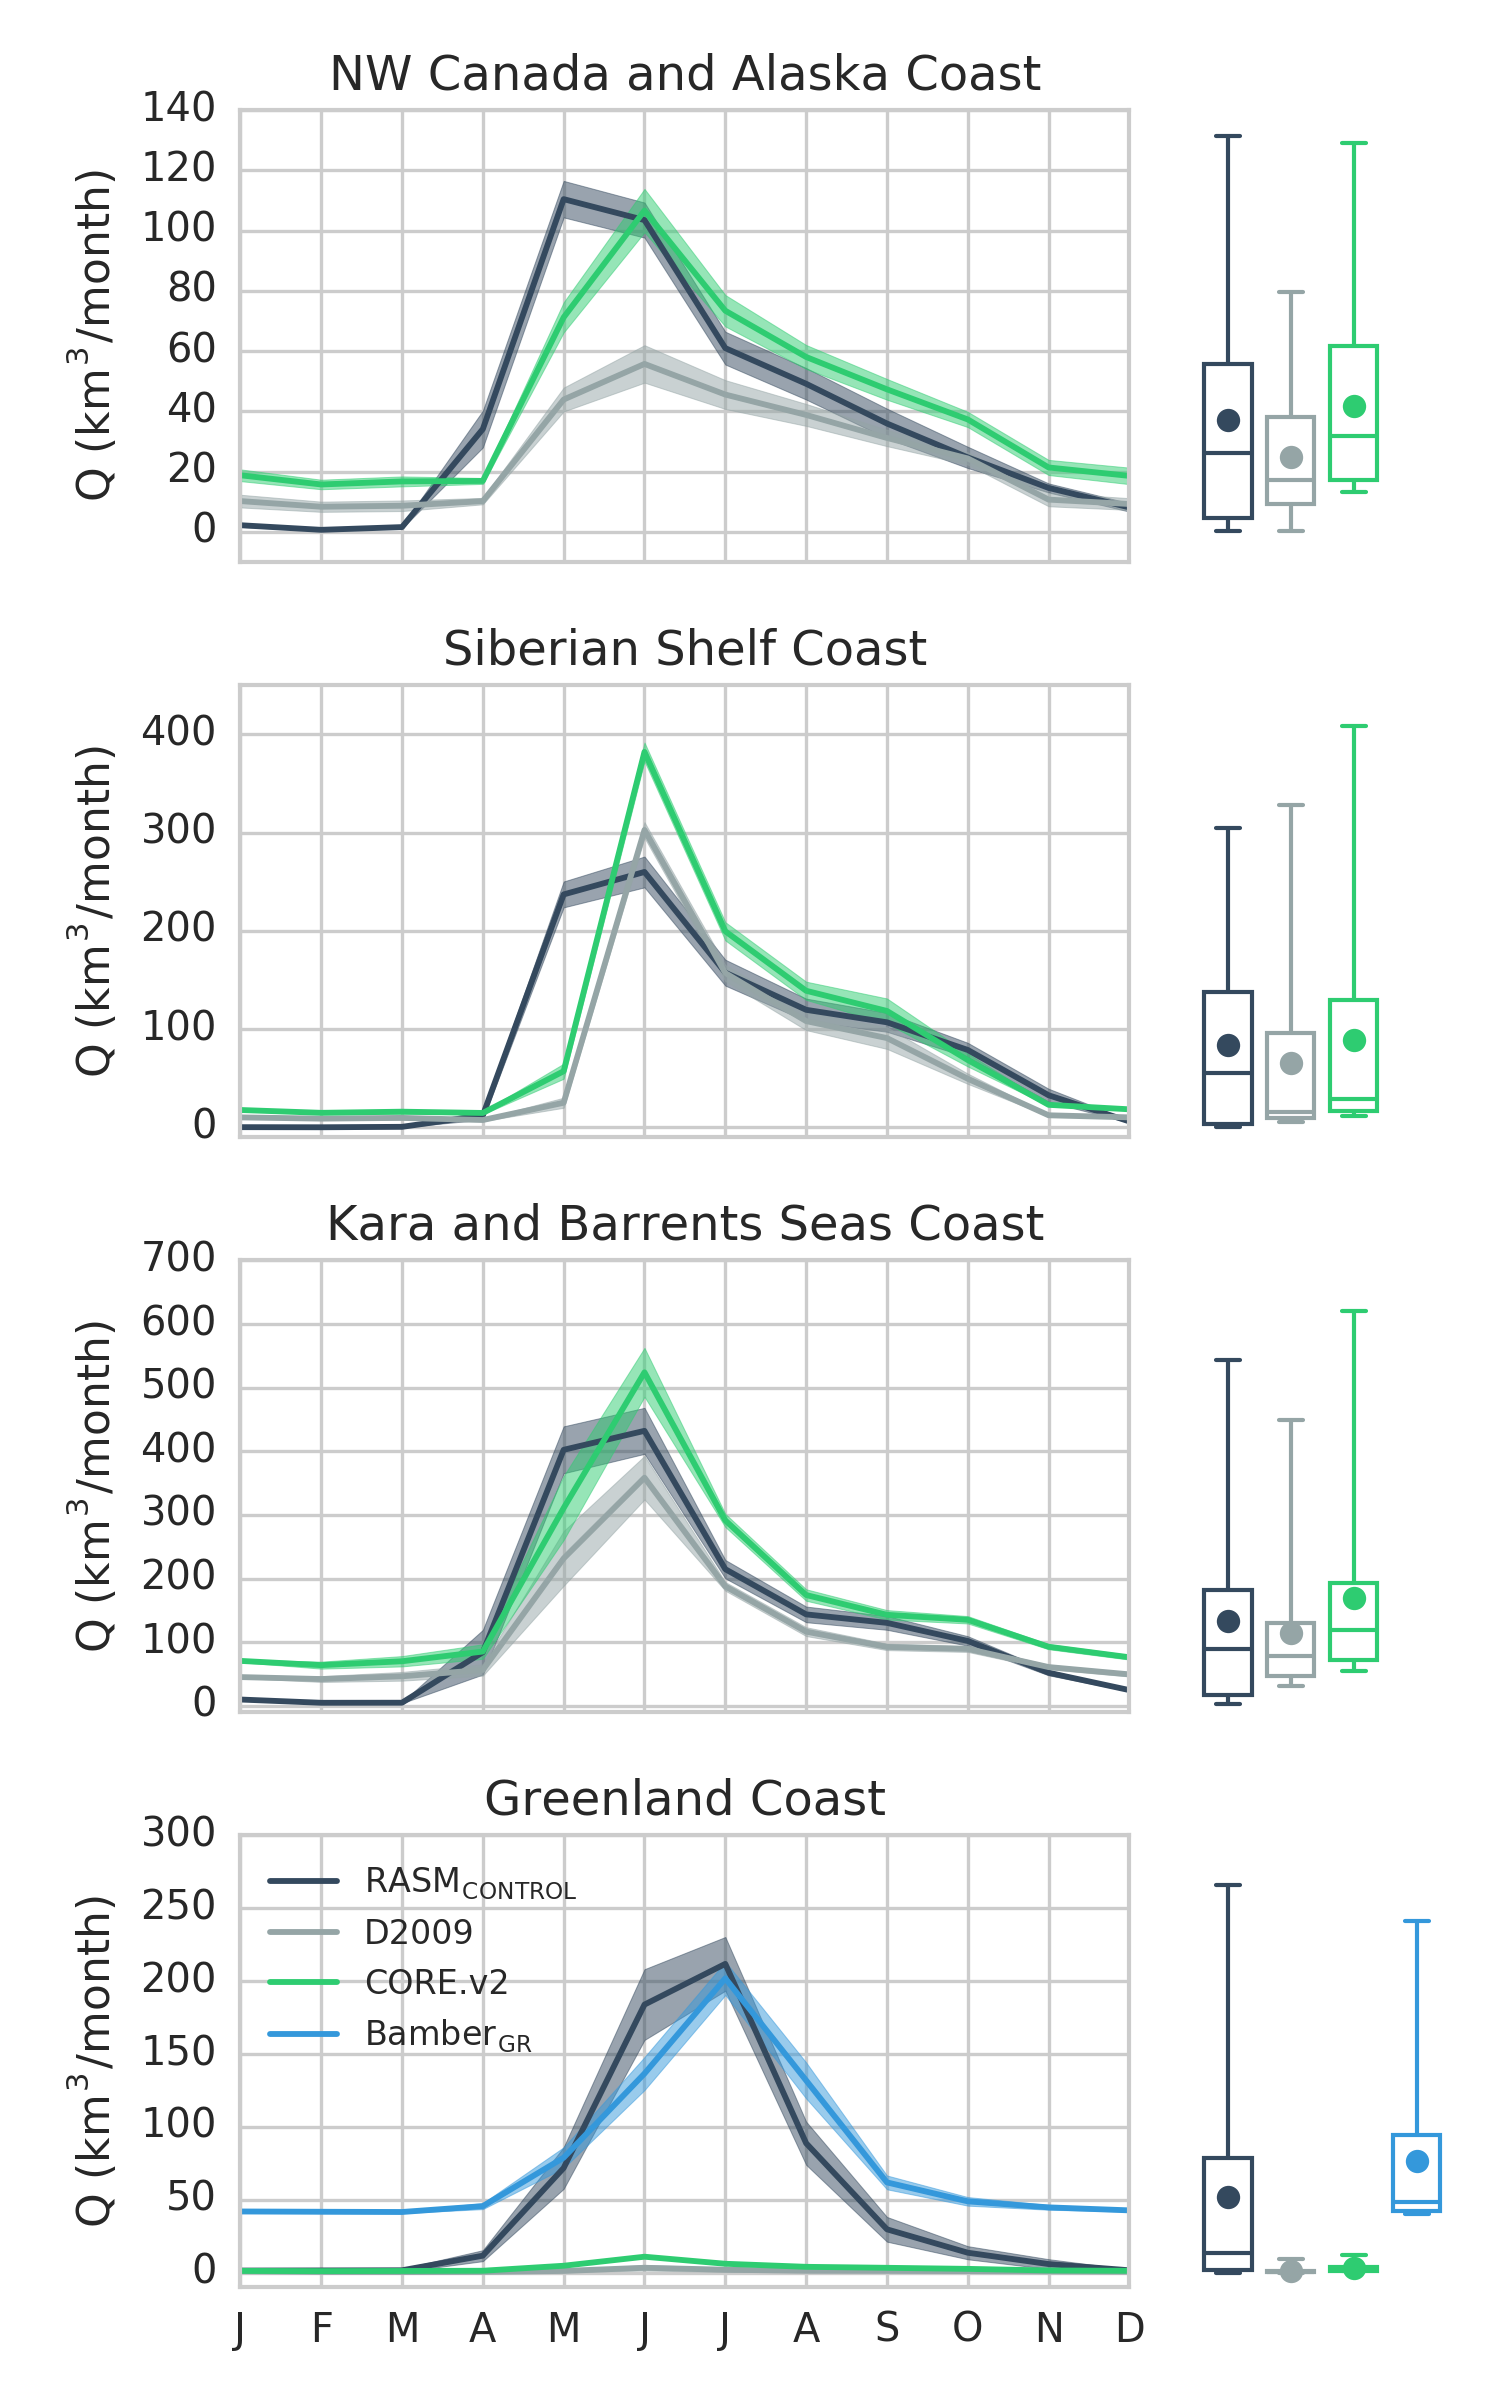
\includegraphics[width=10cm,keepaspectratio]{coastal_hydrographs}
    \caption{Left: Annual cycle of coastal streamflow fluxes for the four masks shown in Figure \ref{fig:rasm_domain} comparing $RASM_{CONTROL}$ (dark blue), $D2009$ (gray), $CORE.v2$ (green), and $Bamber_{GR}$ (light blue, Greenland only).
    Solid lines represent the 1991-1999 mean and the shading denotes the interannual variability.
    Right: Box and whisker from the monthly timeseries.
    Whiskers represent the full data range, circles represent the mean, horizontal lines represent the median, and the box represents the first and third quartiles.
    }
    \label{fig:coastal_hydrographs}
\end{figure}

% [Greenland: RASM vs. CORE II vs. sum of Dai/Trenberth vs. Bamber]
Runoff from Greenland (bottom of Figure \ref{fig:coastal_hydrographs}) is a large contributor to the total coastal freshwater flux in the Arctic region, consisting of approximately 10\% of the total Arctic drainage area.
However, there are no long-term observations of the coastal freshwater flux (liquid streamflow or glacier calving) and global observation datasets (e.g. $D2009$) often ignore this drainage area.
In Figure \ref{fig:coastal_hydrographs}, we compare the coastal freshwater flux from Greenland to the $CORE.v2$ and $D2009$ datasets, as well as to the model estimates from $Bamber_{GR}$.
Because there are no observations over Greenland, the streamflow flux in $D2009$ is zero for all months.
Because $CORE.v2$ relies heavily on observations, their freshwater flux from Greenland is also near zero in all months.
Compared to $Bamber_{GR}$, $RASM_{CONTROL}$ has a similar annual average freshwater flux (see adjacent box and whisker plots) although RASM tends to have more runoff in the spring and less during the winter months.
The solid ice calving flux in $Bamber_{GR}$ is uniformly applied throughout the year, even though observational evidence indicates the existence of a seasonal cycle in this flux as well \citep[e.g.][]{Joughin_2008}.
Applying a seasonal cycle to the solid ice calving flux in $Bamber_{GR}$ fluxes may bring it closer into alignment to $RASM_{CONTROL}$ in both the winter and spring seasons.
In terms of both the annual cycle and mean, the freshwater flux from $RASM_{CONTROL}$ represents a significant improvement, relative to $CORE.v2$ over Greenland.

\section{Discussion}
\label{sec:discussion_ch4}

\subsection{Impacts on the Arctic Climate System}
\label{sec:ocean}
Figure \ref{fig:ocean_timeseries} shows the monthly time series of the streamflow flux to the ocean for the entire domain (left) and the Central Arctic (right) for the $RASM_{CONTROL}$ simulation.
In the Central Arctic basin, the streamflow flux can be greater than 500 km$^3$/month during the melt season and nearly zero during the winter.
As was discussed in section \ref{sec:hydrographs}, the winter streamflow minimum is likely underestimated by VIC due to cold season biases in the baseflow flux.
Figure \ref{fig:ocean_timeseries} also shows the time series of SSS and sea surface temperature (SST).
The SSS in $RASM_{NOROF}$ is in a transient state until about the year 2000 and it represents the adjustment of the Arctic Ocean to having no runoff.
The $RASM_{CONTROL}$ simulation reaches a steady state about 10 years earlier (c. 1990).
The adjustment period in the $RASM_{CONTROL}$ simulation is a result of the change in the atmospheric and streamflow forcings, from $CORE.v2$ (used for the spinup of the ocean model component to provide initial boundary conditions) to coupled within RASM.
The change in salinity during the first ten years of the $RASM_{CONTROL}$ simulation is mainly driven by a change in the streamflow flux (note the difference between $RASM_{CONTROL}$ and $RASM_{NOROF}$) but cannot be completely separated from the change in atmospheric forcings.
By 2010, the SSS differs between the two simulations by about 0.6 ppt (parts per thousand) for the full ocean domain and by 1.5 ppt for the central Arctic basin.
These differences are approximately equal to the annual amplitude of surface salinities in the RASM simulations.
The differences in the SSTs between the two simulations are relatively small when averaged over the full ocean domain, however, the $RASM_{CONTROL}$ simulation is found to be about 0.25 $^{\circ}$C warmer than the $RASM_{NOROF}$ simulation in the central Arctic basin.

\begin{figure}
    \centering
    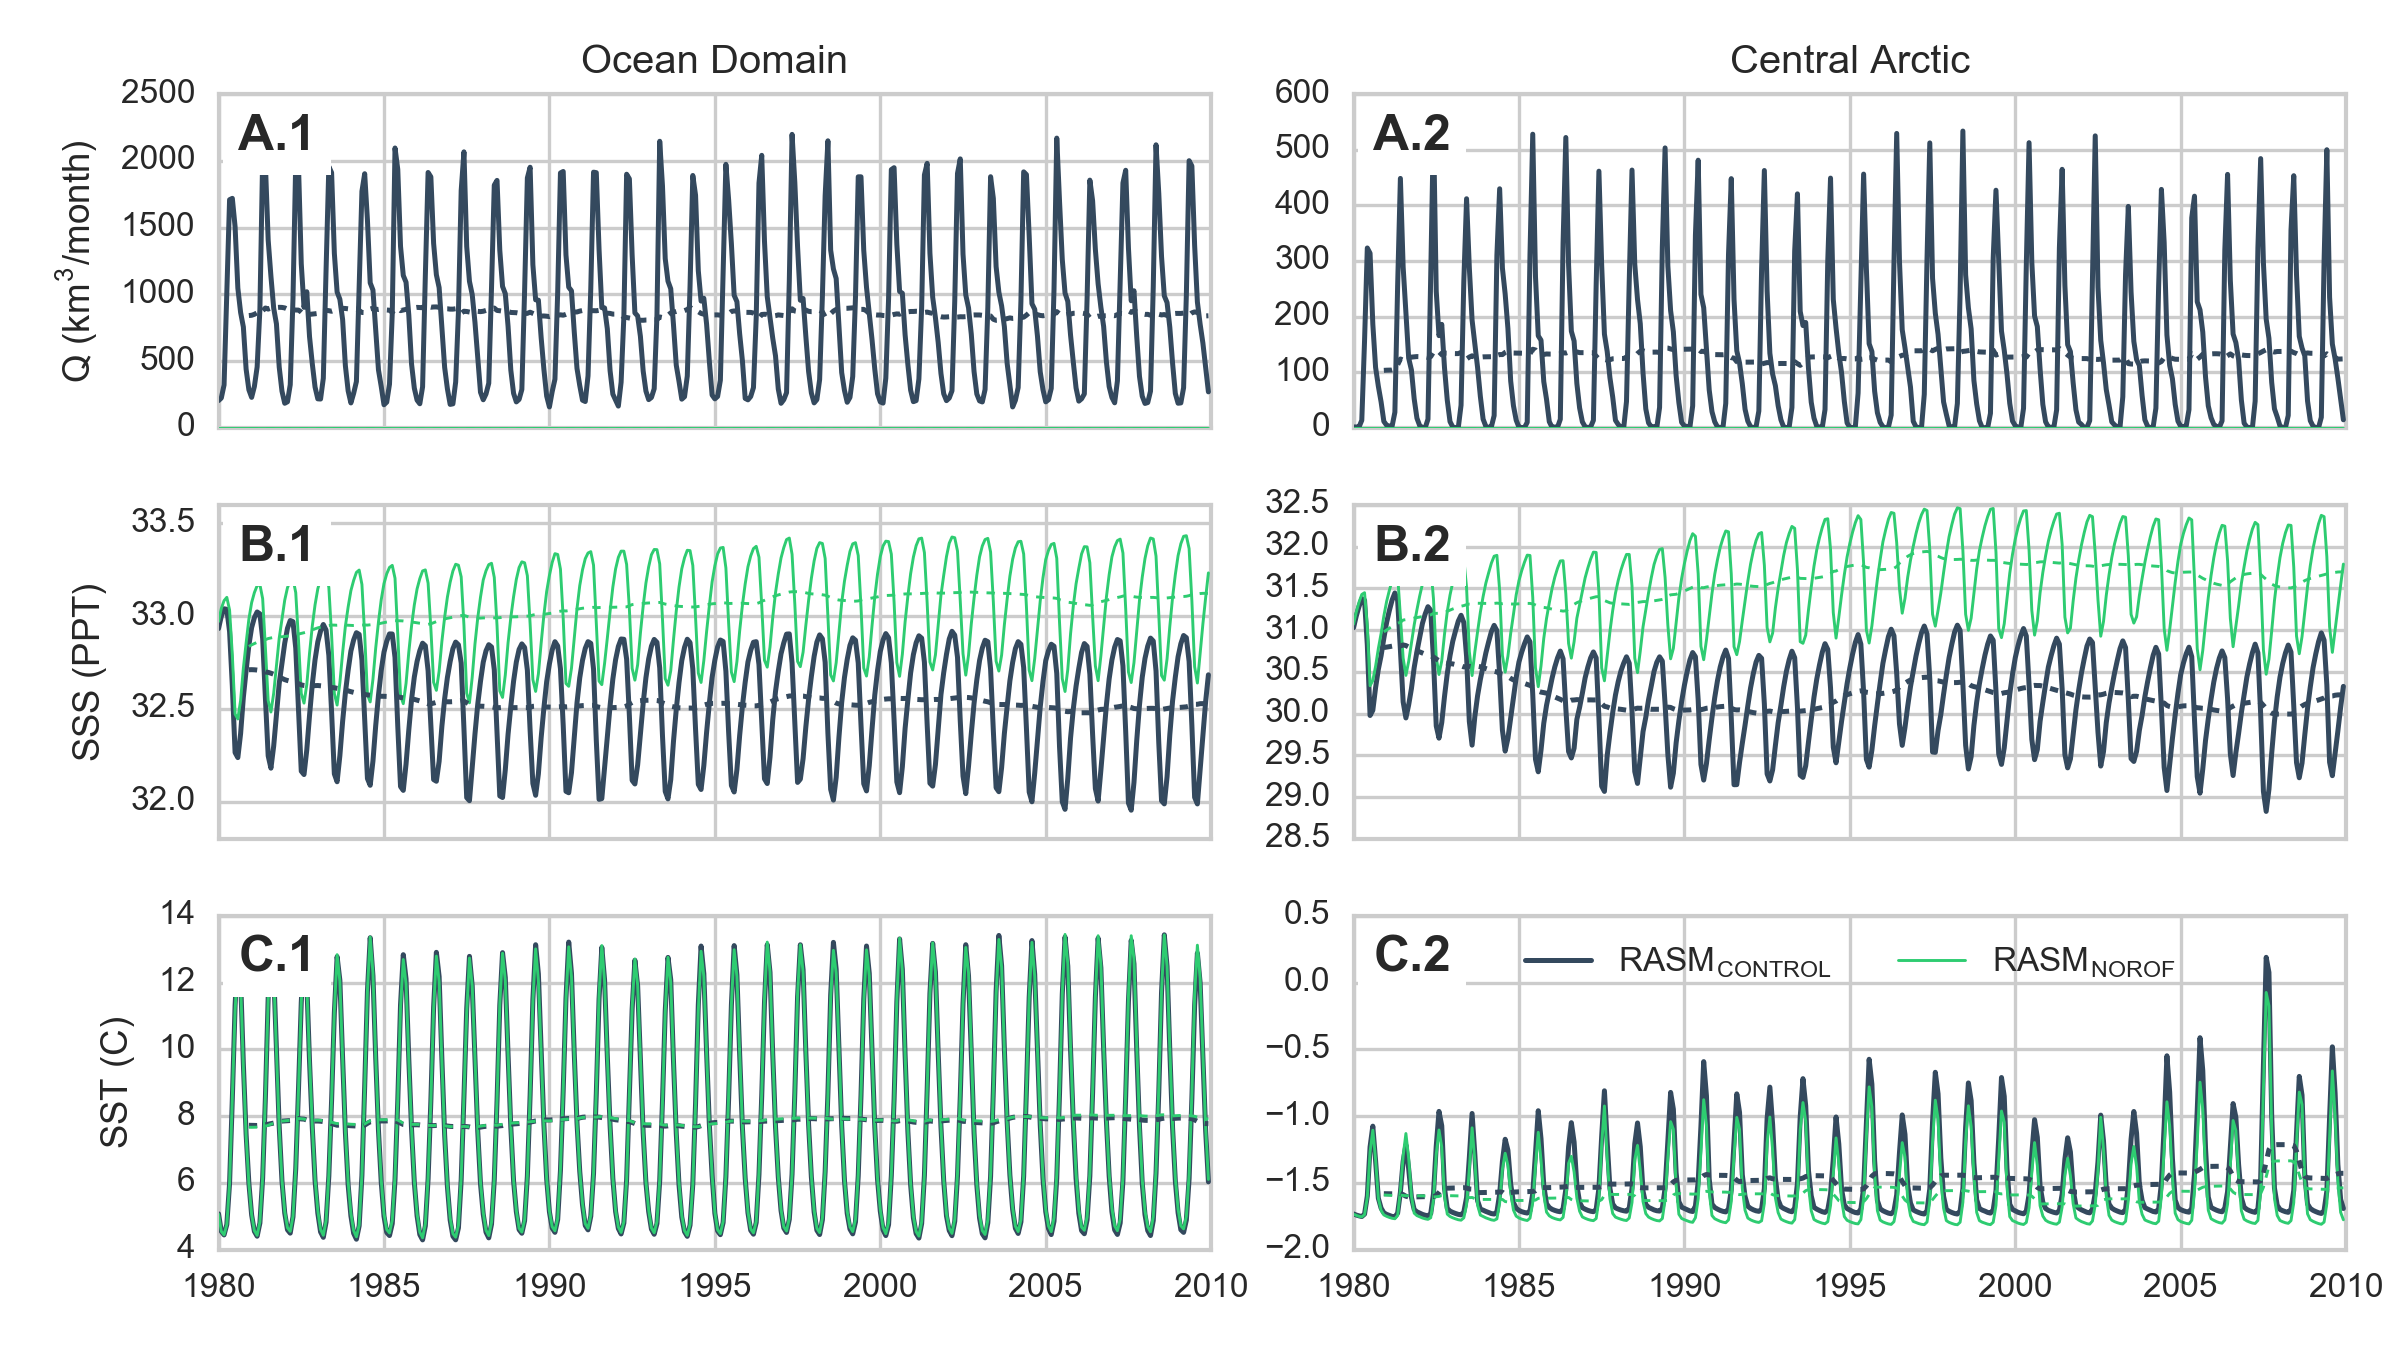
\includegraphics[width=18cm,keepaspectratio]{ocean_combine_ts}
    \caption{Monthly time series (1980-2009) of domain-wide (left) and central arctic (right) streamflow (top; $RASM_{CONTROL}$ only), mean SSS (middle), and SST (bottom) for the $RASM_{CONTROL}$ (blue) and $RASM_{NOROF}$ (green). The dashed lines show a 12-month running mean.
    }
    \label{fig:ocean_timeseries}
\end{figure}

Within the Arctic Ocean, the largest and most direct impact of the streamflow flux is on near coastal SSS.
This impact on SSS is expected to translate to changes in the ocean temperature as well as the distribution of sea ice.
Spatial maps of seasonally averaged SSS, SST, and sea ice thickness differences are shown in Figure \ref{fig:ocean_maps} for the years 2000-2009. This period corresponds to a stable and relatively flat domain-wide SSS and SST signal for the $RASM_{CONTROL}$ case, after adjustment of the model following the 1979 initialization, as indicated in Figure \ref{fig:ocean_timeseries}.

In Figure \ref{fig:ocean_maps}, statistical significance for the difference between the two RASM simulations is calculated with Welc`s two-sided t-test using lag-1 autocorrelation to estimate effective sample size following \citet{VonStorch1999} and \citet{Wilks2006} and stippled at the 95\% confidence interval.
For reference, the observed ice edge (15\% sea ice concentration contour) has been overlayed from the NOAA/NSIDC passive microwave sea-ice concentration climate record of \citep{Meier2013}.
While regions outside of the Central Arctic are not significantly different between the two RASM simulations, the Central Arctic basin is shown to be between 1 and 6 ppt fresher in $RASM_{CONTROL}$ than in $RASM_{NOROF}$.
The differences between the two simulations are largest in closed ocean basins (e.g. Hudson Bay) and along shallow shelves that are adjacent to the outlets of large rivers (e.g. Siberian Shelf and Beaufort Shelf).
Outside the Central Arctic, particularly around the margins of Greenland and in Baffin Bay, there are also large areas where the SSS in $RASM_{CONTROL}$ is considerably lower than in $RASM_{NOROF}$.
The differences in SSS between these two RASM simulations in these areas highlight the local and regional importance of streamflow as a driver of ocean dynamics, and are coherent with the observed impact of increased runoff in the Arctic Ocean \citep [e.g.][]{Morison_2012}.
In the Central Arctic, sea ice thickness for the $RASM_{NOROF}$ simulation is higher in all seasons by up to $\sim$0.5 m.
These differences are largest in the Laptev Sea and along the Kara Shelf, which receive streamflow from the three largest Eurasian rivers.
The differences in sea ice thickness can be partially attributed to an earlier freeze-up in the $RASM_{CONTROL}$ simulation.
The freeze-up timing differences are closely related to the differences in SST, where $RASM_{NOROF}$ is colder in all seasons throughout the central Arctic.
As we discussed in section \ref{sec:intro_ch4}, the earlier freeze-up reduces the amount of heat that can be lost by the ocean in the fall and, over the long-term, leads to reductions in sea ice volume.
This result partially corroborates the findings of \citep{Morison_2012} insofar as they also indicated, from an observational perspective, that a fresher Arctic Ocean would have less sea ice.

\begin{figure}
    \centering
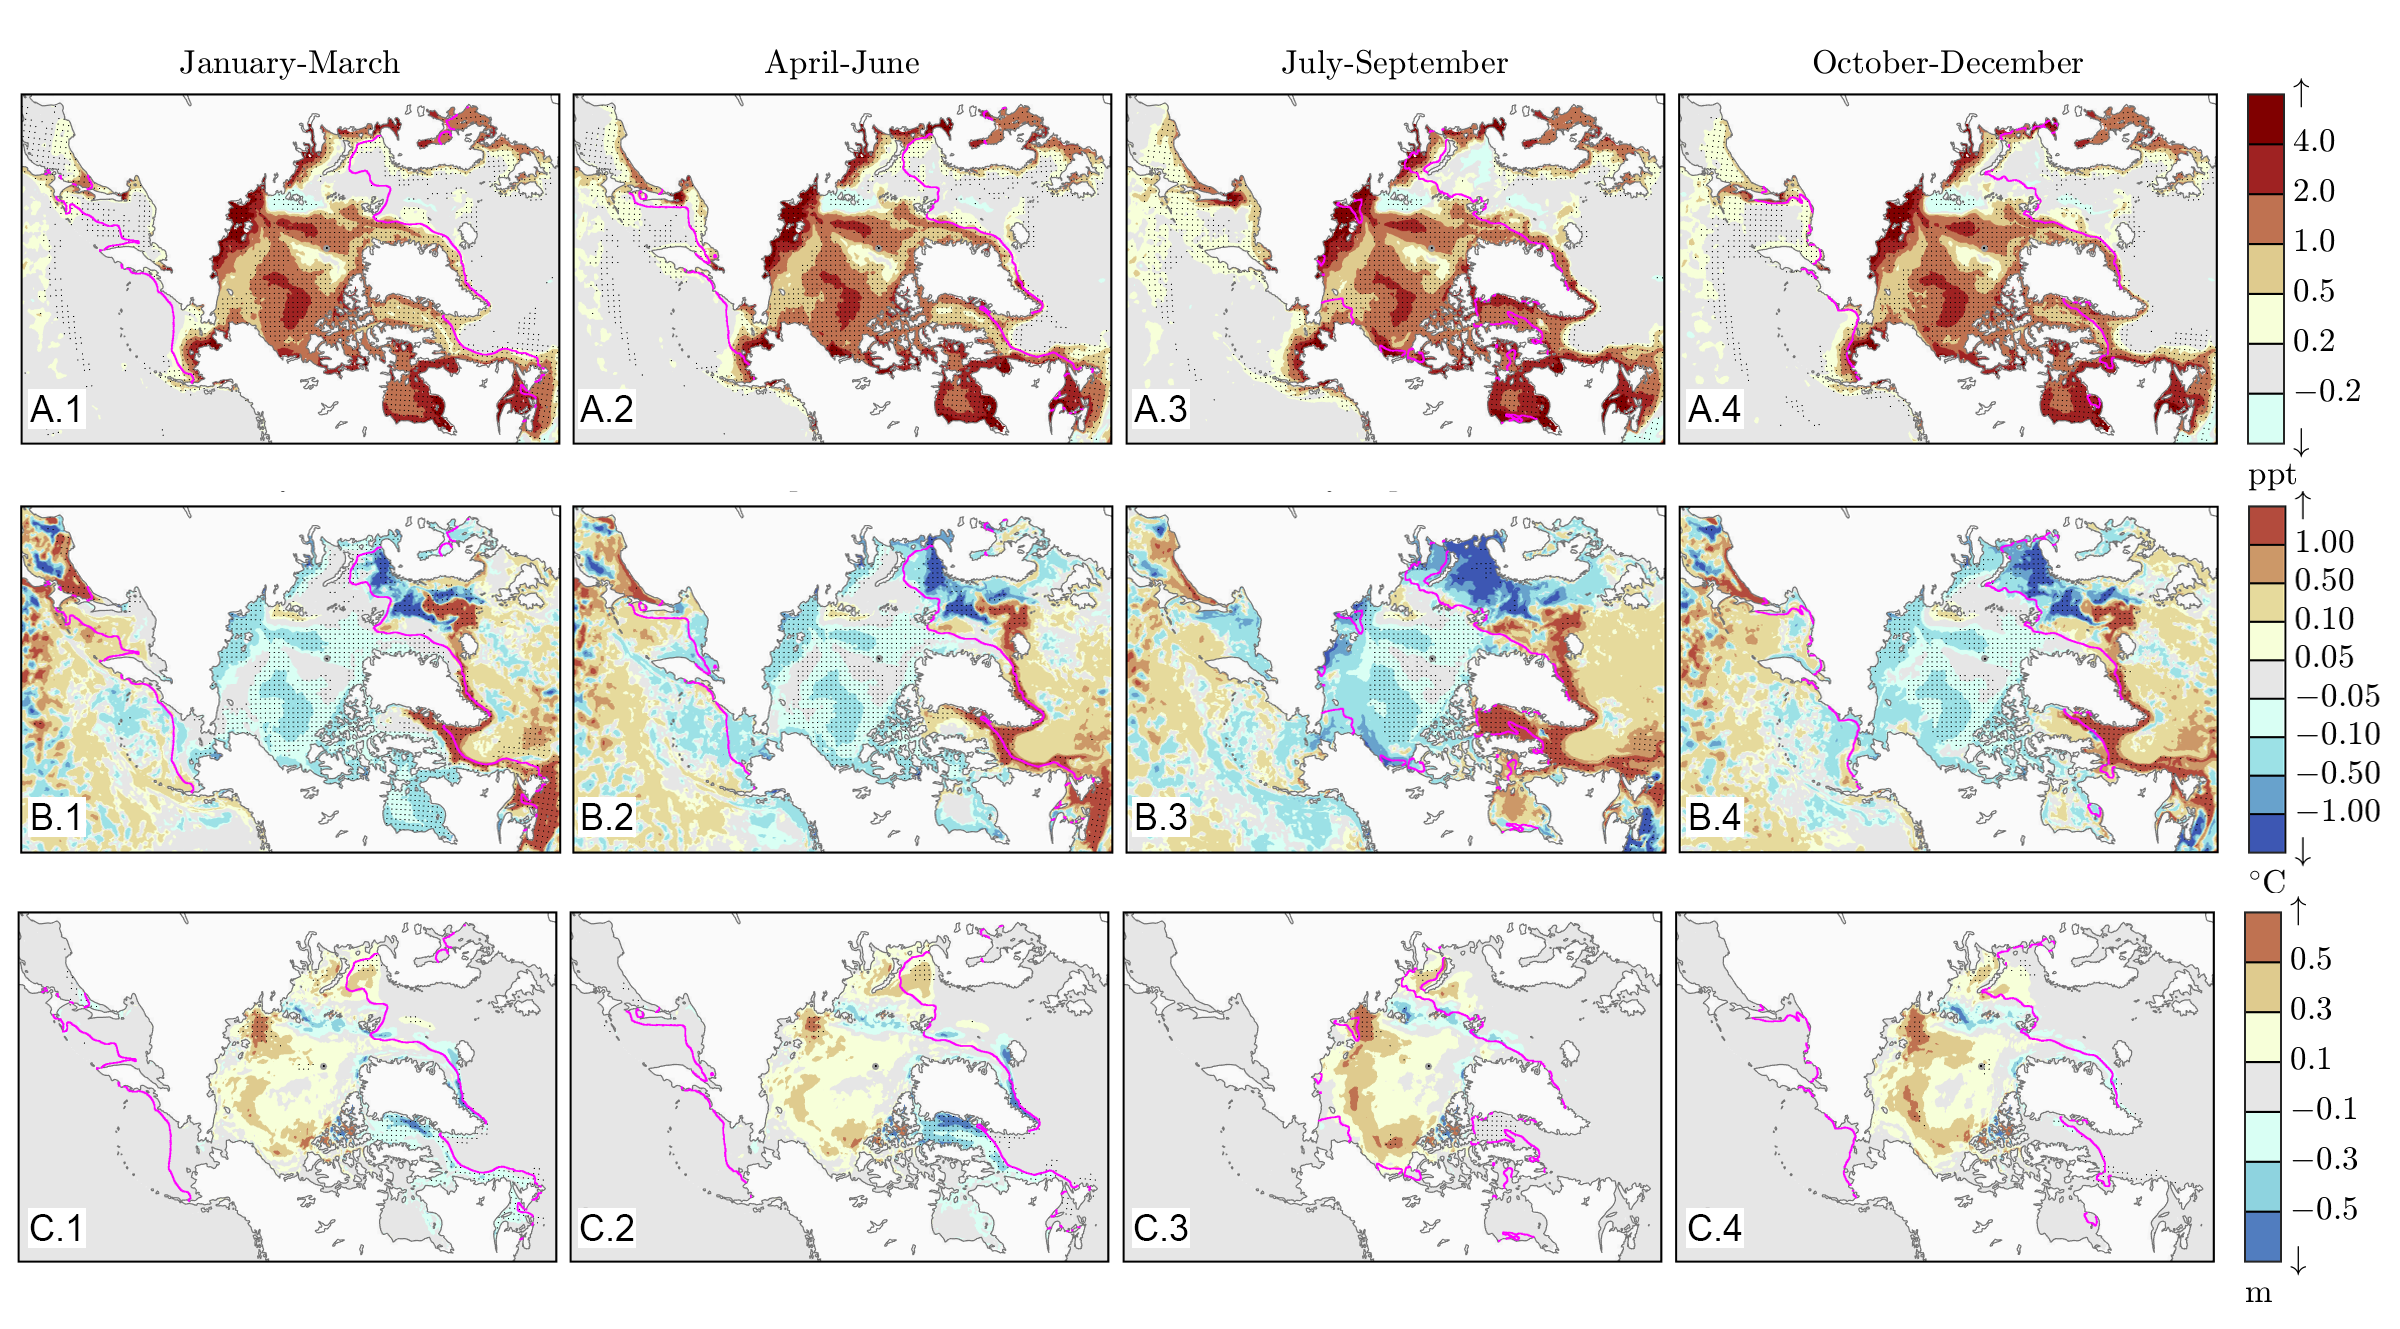
\includegraphics[width=18cm,keepaspectratio]{ocean_combine}
\caption{Seasonal difference ($RASM_{NOROF}$ - $RASM_{CONTROL}$) in mean sea surface salinity (top), sea surface temperature (middle), and sea ice thickness (bottom) (2000-2009). Stippling denotes differences that are statistically significant at the 95\%  confidence interval. The magenta contour represents the observed 15\% sea ice concentration contour. }
\label{fig:ocean_maps}
\end{figure}

\subsection{Routing Processes}

We have shown that RVIC simulates the primary characteristics of the seasonal hydrograph across the Arctic region by capturing the differences in cold and warm season streamflow behavior.
The RVIC model, coupled within RASM, effectively delivers streamflow to all coastal grid points draining to the POP model domain.
We have also demonstrated that the IRFs are relatively easy to parameterize in RVIC through the use of a simple optimization procedure.

While we have shown that RVIC, coupled within RASM, is able to capture the first order behavior of streamflow processes affecting the timing and shape of the annual hydrograph, we recognize it may not be well suited to capture many of the second order processes unique to the Arctic.
For example, there is no mechanism in the RVIC model to account for non-linear routing processes such as overbank flow, wetlands, ice jams, reservoir operations, and industrial or agricultural withdrawals.
\citet{Adam_2007} highlight the importance of representing the reservoir influences to capture the annual hydrograph in the Lena, Yenisei, and Ob' Rivers.
Errors caused by not explicitly representing these processes are apparent, for example, in the Nelson River (bottom of Figure \ref{fig:hydrographs}), where RVIC produces a naturalized hydrograph that bears little resemblance to the observed hydrograph which is highly influenced by reservoir operations.
Ice dam dynamics during the spring melt affect many of the high-latitude rivers and are also not well represented using a linear routing model.
However, due to the timestep of the analysis here, we do not believe these processes contribute significantly to the errors in streamflow timing, nor are they likely to significantly impact the coupling with the ocean model.

While the initial implementation of the RVIC model coupled within RASM completes the freshwater cycle, it does not provide explicit mechanisms to deterministically route other runoff properties, such as heat, nutrients, or sediments.
Previous studies \citep[e.g.][]{vanVliet_2011,vanVliet_2012}, using the original \citet{Lohmann_1996} model, have included representations of water quality and temperature in uncoupled simulations.
\citet{Lammers_2007} used observations to provide an estimate of the heat flux derived from streamflow from the Russian portion of the Arctic basin (0.2 $W/m^2$).
While this heat flux into the Arctic ocean is unlikely to significantly impact the regional ocean energy budget, it may play an important role in the spring melt of sea ice near the outlet of large rivers.

\subsection{Coastal Streamflow Flux Dataset}
Beyond introducing the RVIC streamflow routing model, this paper also describes the associated coastal streamflow flux dataset which has been made publically available.
This dataset includes daily streamflow at all 50-km coastal grid cells in the RASM domain.
Relative to existing coastal streamflow flux datasets used by the ocean modeling community (e.g. $D2009$, and $CORE.v2$), this dataset includes the following improvements:

\begin{itemize}
  \item Spatial resolution: the dataset is provided on a 50-km near equal area stereographic grid which is a finer resolution than existing datasets.
  \item Temporal resolution: the dataset includes mean daily streamflow fluxes between September 1, 1979 and December 31, 2014. Limited by the monthly availability of the observations in $D2009$, $CORE.v2$ only included mean monthly streamflow fluxes.
  The higher temporal frequency of this dataset will better represent hydrologic extremes such as floods and low flows, and may enable improved mesoscale process representation in ocean models (e.g. eddies, freshwater plumes).
  \item Self-consistent: Blended forcing datasets that combine model results with observations often include spatial and temporal inconsistencies as well as non-uniform biases. We have shown that the RVIC model in RASM adequately reproduces the observed streamflow hydrograph. Because the streamflow routing in gauged and ungauged regions is done identically within RASM, this dataset should be expected to have similar performance in ungauged areas.
  \item Greenland fluxes: In section \ref{sec:coastal_streamflow}, we highlighted the improved representation of the freshwater flux from Greenland. Although RASM does not include a dynamic ice-sheet model like the one used in the development of $Bamber_{GR}$, the snowmelt and streamflow routing behavior is a significant improvement, relative to $CORE.v2$.
\end{itemize}

\section{Conclusions}
\label{sec:conclusions_ch4}

The RVIC streamflow routing model is a sink-to-source river routing scheme that has been coupled within the Regional Arctic System Model, completing the hydrologic cycle between the land and ocean model components.
In this paper, we have introduced the RVIC model, demonstrated its ability to simulate the first-order routing processes in the Arctic, shown the  importance of the runoff flux in a coupled ocean modeling application, and provided a new dataset of spatially consistent high-resolution coastal streamflow fluxes for ocean modeling.
In doing so, we conclude the following:

\begin{itemize}
  \item Linear routing models, such as RVIC, can be applied within coupled model frameworks to provide high temporal and spatial frequency runoff to ocean models.
  RVIC is computationally inexpensive and is relatively easy to parameterize, two features that add to its applicability in a wide range of coupled climate modeling applications.
  \item Using the remapping and upscaling approach of IRFs described in section ~\ref{sec:remap}, we introduced a new method for developing IRFs using dissimilar flow direction and routing grids.
  From an implementation perspective, this flexibility greatly expands RVIC's utiity for a range of modeling applications using arbitrarily shaped LSM grids, including irregularly shaped polygons (e.g. sub-basin scale hydrologic response units).
  Although not specifically discussed in this paper, we hypothesize that this method preserves the small-scale routing behavior while facilitating routing to be done on a coarser land surface grid.
  This point may warrant additional evaluation in follow-up studies.
  \item A relatively simple optimization procedure can provide significantly better routing model performance.
  Of course, a more thorough parameter selection procedure could be envisioned in which watersheds would be calibrated individually using spatially-distributed velocity and diffusivity parameters derived directly from original sources (e.g. digital elevation models).
  However, the spatial and temporal scales of interest in this study did not warrant this level of optimization.
  \item More complex routing schemes are likely required to adequately capture additional fluxes related to streamflow routing.
  In our discussion, we have highlighted the fact that RVIC is not particularly well suited to handle the routing of additional quantities such as stream temperature, nutrients, or sediments.
  We recognize that the representation of these quantities may be important to a range of biogeophysical processes in the near-surface ocean in coupled models.
  New, more complex, and physically based routing models, such as the recently developed MOSART model \citep{Li_2013}, offer some potential to provide additional process representation.
  The obvious challenge with these models is developing and tuning the required input parameters across large, data-spare regions.
  \item The presence of runoff in the RASM ocean and sea ice system has led to decreased SSS, increased SSTs, and decreased sea ice thickness in the Central Arctic basin.
  This result aligns with the findings of observational studies \citep[e.g.][]{Morison_2012}.
  \item We have produced a self-consistent high-resolution (spatial and temporal) coastal streamflow dataset for the Pan-Arctic region.
  Ungauged areas show particularly large improvements relative to $CORE.v2$.
  The dataset is provided at a daily timestep in netCDF file format for the dates between September 1, 1979, and December 31, 2014.
\end{itemize}

{\bf Acknowledgments}
This research was supported under United States Department of Energy (DOE) grants DE-FG02-07ER64460 and DE-SC0006856 to the University of Washington, and DE-SC0005783 and DE-SC0005522 to the Naval Postgraduate School.
Supercomputing resources were provided through the United States Department of Defense (DOD) High Performance Computing Modernization Program at the Army Engineer Research and Development Center and the Air Force Research Laboratory.
The dataset described in this paper is publicly available via the University of Washington (https://digital.lib.washington.edu/researchworks).

%
\chapter{On the relationship between Arctic winter precipitation and minimum sea ice extent}
\label{chap:winter_prec}

This chapter is to be submitted to \textit{Geophysical Research Letters} as

\hangbibentry{Hamman_2016f}

\section*{Abstract}

Over the past three decades, the Arctic has experienced large declines in summer sea ice cover, permafrost extent and spring snow cover, as well as increases in winter precipitation.
This study explores the relationship between declining Arctic sea ice extent and early winter precipitation across the high-latitude Arctic land masses.
The first part of this paper presents the observed relationship between sea ice extent and winter precipitation.
Using satellite estimates of sea ice extent and precipitation data based on a combination of in-situ observations and global reanalyses, we show that early winter precipitation is negatively correlated with summer sea ice extent and that this relationship is strongest before the year 2000.
After 2000, around the time sea ice extent minima began to decline most rapidly, the relationship between sea ice extent and early winter precipitation degenerates.
This indicates that other processes are driving changes in sea ice extent and winter precipitation.
We hypothesize that the observed correlations between sea ice extent and high winter precipitation are related to anomalous patterns in ocean evaporation and sea ice extent in the fall.
To better understand the physical mechanisms driving the observed changes in the Arctic climate system and the sensitivity of the Arctic climate system to declining sea ice, we have used the fully-coupled Regional Arctic System Model (RASM) to simulate three distinct sea ice climates.
The first climate represents normal sea ice extent, while the second and third represent reduced summer sea ice extent.
The second part of this paper analyzes these three RASM simulations, in conjunction with our observation-based analysis, to understand the relationship between poleward moisture transport, sea ice extent, evaporation from the Arctic Ocean, and precipitation.
We will present the RASM-simulated Arctic water budget and demonstrate the role of sea ice extent in driving winter precipitation anomalies.
Finally, we use the Self-Organizing Map (SOM) machine learning technique to identify characteristic patterns of ocean evaporation, sea ice extent, and polar cap convergence that contribute to anomalies in early winter precipitation.

\section{Introduction}
\label{sec:intro_ch5}

In the past three decades, the Arctic region has experienced unprecedented changes in key cryospheric processes.
Rapid declines in sea ice cover have been accompanied by reductions in permafrost extent and spring snow cover, as well as increases in winter precipitation and winter snow accumulations \citep{Kohler_2006,Callaghan_2011,Bulygina_2009}.
These combined changes have had a marked impact on the regional and global climate systems.
Driving much of these changes has been a regional warming trend that is nearly twice as large as the global mean \citep{Serreze_2006c,Screen_2010}.
This disparity in temperature increases is often referred to as Arctic Amplification and is largely explained by the ice-albedo feedback \citep{Curry_1995}.
While this is likely the primary mechanism that leads to rapid warming in the Arctic, other, secondary feedback processes are also at play.
One such feedback process relates the state and fluxes of the Arctic Ocean (sea surface temperatures or SSTs, sea ice cover, evaporation) to precipitation over land, which modulates winter snow cover and permafrost health.

Observational evidence of an amplified hydrologic cycle \citep{Stocker_2005} has been found in the form of increasing precipitation \citep{Rawlins_2006}, runoff \citep{Peterson_2002}, and winter snow accumulations \citep{Kohler_2006,Bulygina_2009}.
While global average precipitation is expected to increase following a response to warming via the Clausius-Clapeyron relationship \citep[e.g. ][]{Held_2006,Stephens_2008,Byrne_2015}, precipitation increases in the Arctic are expected to exceed the global average \citep{Stocker_2005}.
Analysis of the collection Earth system models (ESMs) in the Coupled Model Intercomparison Project Phase 5 \citep[CMIP5; ][]{Taylor_2012} by \citet{Bintanja_2014} indicates that annual precipitation changes in the Arctic may exceed 50\%, with the largest relative increases in the winter over the Arctic Ocean when precipitation has typically been low.
\citet{Bintanja_2014} also identify that most of these changes are due to precipitation sourced from enhanced local evaporation related to retreating sea ice.
This somewhat contradicts previous work that suggested increased poleward moisture transport as the main driver of Arctic precipitation increases.
Combined with the large intermodel spread of precipitation changes in their study, this contradiction brings into question the sensitivity of the response of Arctic precipitation to reduced sea ice in modern ESMs.
ESMs, along with statistical models, tend to poorly represent the observed decline in summer sea ice extent.
This is evidenced by the intermodel spread among the 39 ESMs analyzed by \citet{Bintanja_2014}.
In their study, changes in sea ice extent between the beginning and end of the twenty-first century ranged between 31-66\%, while changes in precipitation varied by a factor of three to four.

Conceptually, a warmer Arctic Ocean with less sea ice will lead to increased surface evaporation and may lead to enhanced divergence of moisture onto land in the form of precipitation.
Because high-latitude land areas are predominantly below freezing in the fall, increases in precipitation during this season are expected to produce deeper snow packs.
This process would then act to insulate the underlying ground during winter and suppress cold season cooling of high-latitude permafrost \citep{Osterkamp_1999,Zhang_2005,Lawrence_2010}.
Further permafrost degradation may be attributed to earlier spring snow melt driven by regional warming and possibly by increased surface infiltration of warm meltwater \citep{Lawrence_2010}.

How the Arctic climate will respond to such large temperature and sea ice changes has been at the forefront of recent studies \citep[e.g. ][]{Kazutoshi_2014,Simmonds_2014,Wegmann_2015,Vihma_2014}.
Here, we investigate the relationship between Arctic winter precipitation, ocean evaporation, and sea ice extent to better understand the terrestrial precipitation response to the ongoing sea ice decline.
Our a priori hypothesis is that the reductions in sea ice extent would lead to increases in evaporation from the central portions of the Arctic Ocean and precipitation over land during the fall and early winter months.
We explore this hypothesis using three simulations spanning a range of sea ice climates from a fully-coupled regional ESM described in Section \ref{sec:data_models_ch5}.
In Section \ref{sec:results_ch5} we present our analysis of these simulations, first computing the regional freshwater budget following \citet{Serreze_2006a}, then using the Self-Organizing Map (SOM) machine learning technique for dimension reduction and pattern evaluation \citep{Kohonen_1998,Hewitson_2002}.

\section{Data and Methods}
\label{sec:data_models_ch5}

\subsection{Models}
\label{sec:models}
We use three simulations from the Regional Arctic System Model \citep[RASM; ][]{Hamman_2016a,Roberts_2015a}.
RASM is a high-resolution, fully-coupled regional ESM that has been recently developed to improve the representation of coupled Arctic processes.
RASM is comprised of individual land \citep[see ][]{Hamman_2016a}, atmosphere \citep[see ][]{Cassano_2016}, ocean \citep[see ][]{Roberts_2015a}, sea ice \citep[see ][]{Roberts_2015a}, and runoff \citep[see ][]{Hamman_2016b} components, coupled via the CESM flux coupler \citet{Craig_2011}.
In RASM, the atmosphere is forced at its lateral boundaries with the ERA-Interim Reanalysis \citep{Dee_2011} and the ocean's closed boundaries are relaxed to the climatology from \citet{Steele_2001}.
It is important to note that spectral nudging is applied to temperature and winds in RASM above 500 hPa.
From a practical perspective, this nudging means that the synoptic scale circulation patterns in all three RASM simulations closely match those of ERA-Interim \citep{Glisan_2013}.
The land, atmosphere, and runoff components in RASM are applied on a 50 km near equal area polar stereographic grid while the ocean and sea ice are applied on a 1/12$^{\circ}$ rotated pole mesh.

Each of the three RASM simulations used here were run from September 1, 1979 through December 31, 2014, although our analysis begins after a 10-year spinnup to allow for the stabilization of the ocean and sea ice components under coupled forcings.
\citet{Hamman_2016b} provide a complete description of the configuration of RASM for the baseline $RASM_{CONTROL}$ simulation.
Two sensitivity simulations, $RASM_{RSI}$ and $RASM_{RSH}$, representing intermediate and high reductions in sea ice extent are also analyzed.
The configuration of these simulations is identical to $RASM_{CONTROL}$ except in the parameterization of sea ice albedos, which is summarized in Table \ref{table:sims}.
Sea ice albedo is reduced in both simulations to promote accelerated spring sea ice melt and reduced sea ice extent in the summer and fall.
This method of altering the radiative properties of sea ice allows for fully-coupled, self-consistent simulations in RASM and avoids issues with prescribing unphysical surface conditions.

\begin{table}[]
    \centering
    \caption{Summary of RASM simulations used in this chapter.}
    \label{table:sims}
    \begin{tabular}{|l|p{4in}|}
    \hline
    \textbf{Dataset} & \textbf{Sea Ice / Ocean Configuration}                                                                                                         \\ \hline
    $RASM_{CONTROL}$    & Default RASM (see \citet{Hamman_2016b})                                                                                                          \\ \hline
    $RASM_{RSI}$         & \begin{tabular}[c]{@{}l@{}}Ocean: No changes\\ Sea Ice: Snow albedo -0.5 std. dev. of observed.\end{tabular}                                   \\ \hline
    $RASM_{RSH}$         & \begin{tabular}[c]{@{}p{3.5in}}Ocean: No changes\\ Sea Ice: No sea ice initial condition, reduced snow/ice/pond albedo -2.0 std. dev.
    \end{tabular} \\ \hline
    \end{tabular}
\end{table}

\subsection{Datasets}
\label{sec:data}
Observations of sea ice extent are taken from the National Snow and Ice Data Center (NSIDC) Weekly Sea Ice Extent product \citep{Brodzik_2013}.
Gridded precipitations observations between 1979 and 2014 are taken from CRU TS v.3.23 \citep{Harris_2014}.
We also used monthly mean precipitation data ERA-Interim \citep[referred to hereafter as ERA; ][]{Dee_2011} and NASA’s Modern-Era Retrospective Analysis for Research and Applications \citep[MERRA; ][]{Rienecker_2011}.
These two datasets, originally provided at their respective native resolution of 0.75$^{\circ}$x0.75$^{\circ}$ and 0.5$^{\circ}$ x 0.667$^{\circ}$ spatial resolutions, were resampled to RASM's land/atmosphere grid for use in this study.

\subsection{Self-Organizing Maps}
In Section \ref{sec:rasm_results}, we present results using the Self-Organizing Map \citep{Kohonen_1998,Hewitson_2002} technique.
SOMs are a useful technique for dimension reduction, allowing for the identification of unique climatological patterns.
They are are a type of unsupervised machine learning, utilizing artificial neural networks to create a lower-dimensional representation of high-dimensional datasets.
SOMs have been previously applied in studies of polar climatology to study synoptic scale atmospheric circulation \citep[e.g. ][]{Cassano_2007}, extreme weather events \citep[e.g. ][]{Cassano_2015,Glisan_2016}, and coupled ocean-atmosphere processes \citep[e.g. ][]{DuVivier_2016}.

In our analysis, we trained a 2x4 SOM, using standardized ocean evaporation anomalies north of 55$^{\circ}$ N from each of the three RASM simulations described in Section \ref{sec:models} for individual fall months (October - December) between 1985 and 2014.
In total, the training dataset was comprised of 270 months of evaporation anomalies.
Standardized anomalies were calculated using the climatology calculated from the entire analysis period.
We used a evaluation metric of Euclidean distance, a learning rate of 0.001, and a maximum number of iterations of 2000.
The shape of the 2x4 SOM was chosen to provide a sufficient number of unique patterns while maximizing the average number of samples in each pattern.
% BN: Should the training domain be limited to that of Figure 4?  % JH: I have tried that and we can go over those results. I remember them not being particularly easy to understand.
The SOM was initialized with random fields from a standard normal distribution. % BN: This doesn't mean much to people who have not used SOMs. What is the implication of this choice for initialization?
% JH: True, but since there are other ways to initialize a som, I think it is important that we state our methodology.
% BN: Are all cells independent?
% JH: No. The each month is put into an individual node.
Further details on the SOM algorithm can be found in \citet{Reusch_2005} or \citet{Cassano_2015}.

\section{Results and Discussion}
\label{sec:results_ch5}
\subsection{Observational evidence}
% Motivation and establishing a connection between sea ice extent and precipitation
Our hypothesized relationship between precipitation and sea ice extent builds on the observed interannual covariation of precipitation and sea ice extent across the central Arctic drainage basin.
Here we define the central Arctic drainage basin as the land areas draining to the core sea ice regions of the Arctic ocean, including the Siberian Shelf (mainly the Kolyma and Lena Rivers) and Canadian coast (mainly the Mackenzie River).
% BN: A figure would help in describing the central arctic. You can probably overlay this on Figure 2 or just refer to Figure 4.
Figure \ref{fig:prec_ice_ts} presents the timeseries of observed annual minimum sea ice extent and October-December precipitation in the central Arctic drainage basin from the MERRA and ERA reanalysis and CRU datasets.
Using the Spearman rank-order correlation measure \citep{Spearman_1904}, the MERRA, ERA, and CRU datasets exhibit correlations of -0.38, -0.40, and -0.52 respectively.
The observed relationship (i.e., negative correlations) is most prominent prior to 2000.
This raises the question whether the two processes are related through a physical coupling that is limited by a threshold mechanism or whether they are perhaps driven by a common forcing.

\begin{figure}
  \centering
  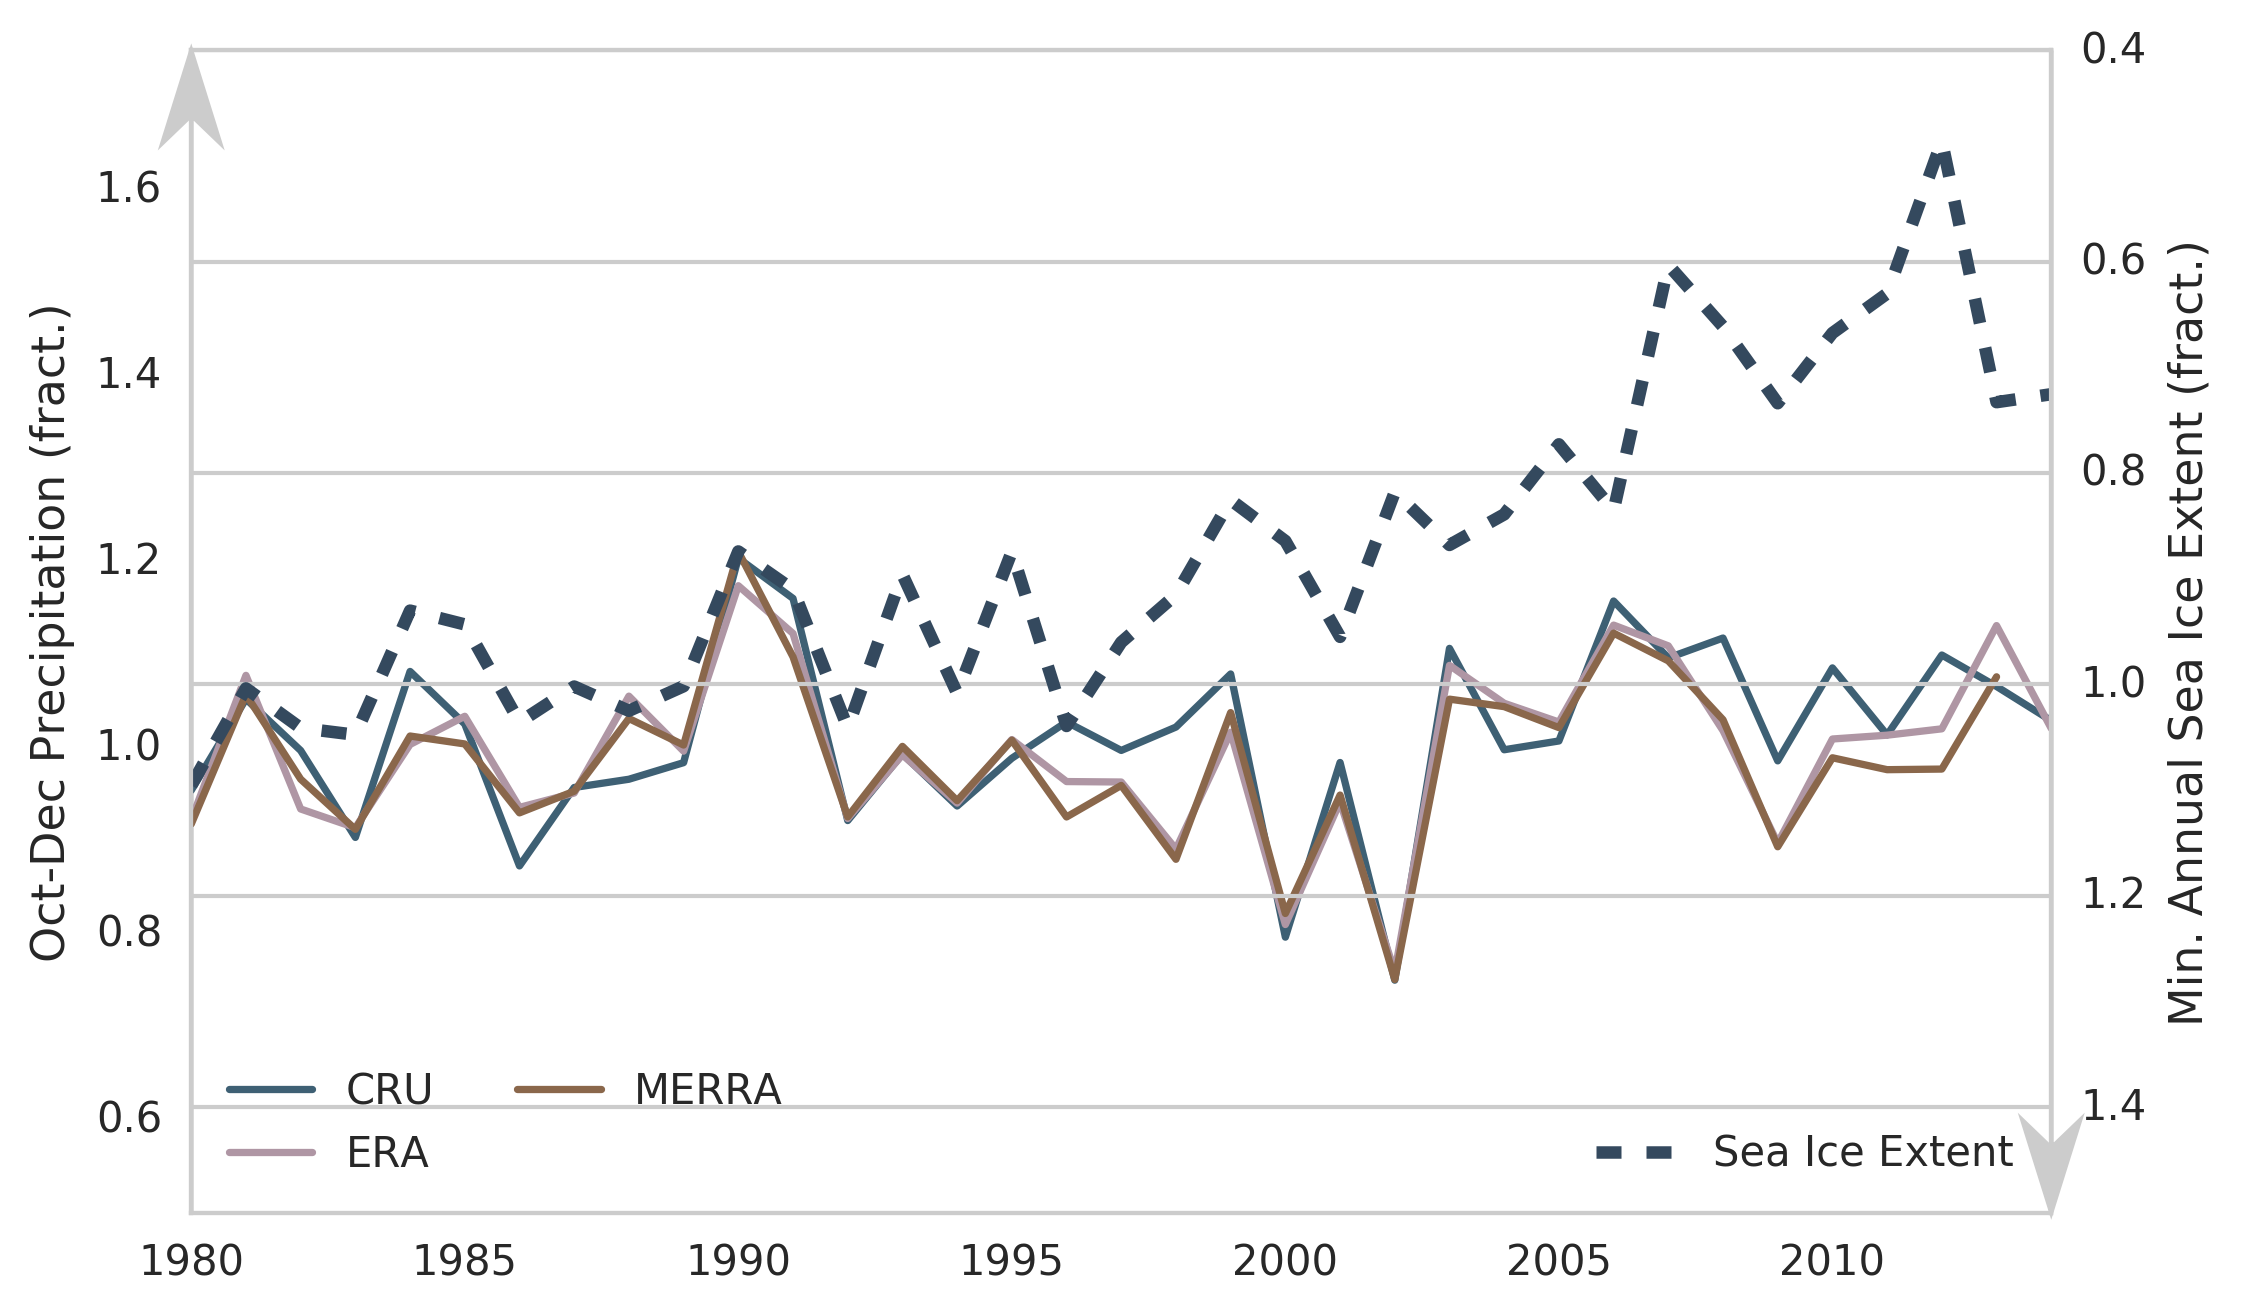
\includegraphics[width=12cm,keepaspectratio]{prec_seaice_ts}
  \caption{Timeseries (1980-2015) of fall precipitation (Oct - Dec) over the central Arctic drainage basin, (left axis) compared to minimum annual sea ice extent (right axis). Note that the right axis is inverted. Units for both axes are fraction of the 1980-1990 mean.}
  \label{fig:prec_ice_ts}
\end{figure}

Figure \ref{fig:prec_spatial_corr} shows the Spearman rank-order correlation coefficients between minimum annual sea ice extent and October-December precipitation from the CRU dataset at each grid cell within the RASM domain.
Across most of the domain, the correlations are found to be below zero, with the most negative correlations occurring across Siberia and North America.
Correlations across northern Europe are predominantly near zero or positive. % BN: But is Europe part of the central Arctic drainage as you describe it earlier? I think you need to mask these figures to ONLY show the part that is actually used in analysis (the lines in Figure 1).
% JH: I've masked the spatial figure for the RVIC drainage and just called out the northern Europe piece.
Generally, a moderately consistent relationship exists between sea ice extent and precipitation, especially in the high-latitude regions of the study domain.
In the following sections, we will investigate possible mechanisms for this relationship.

\begin{figure}
  \centering
  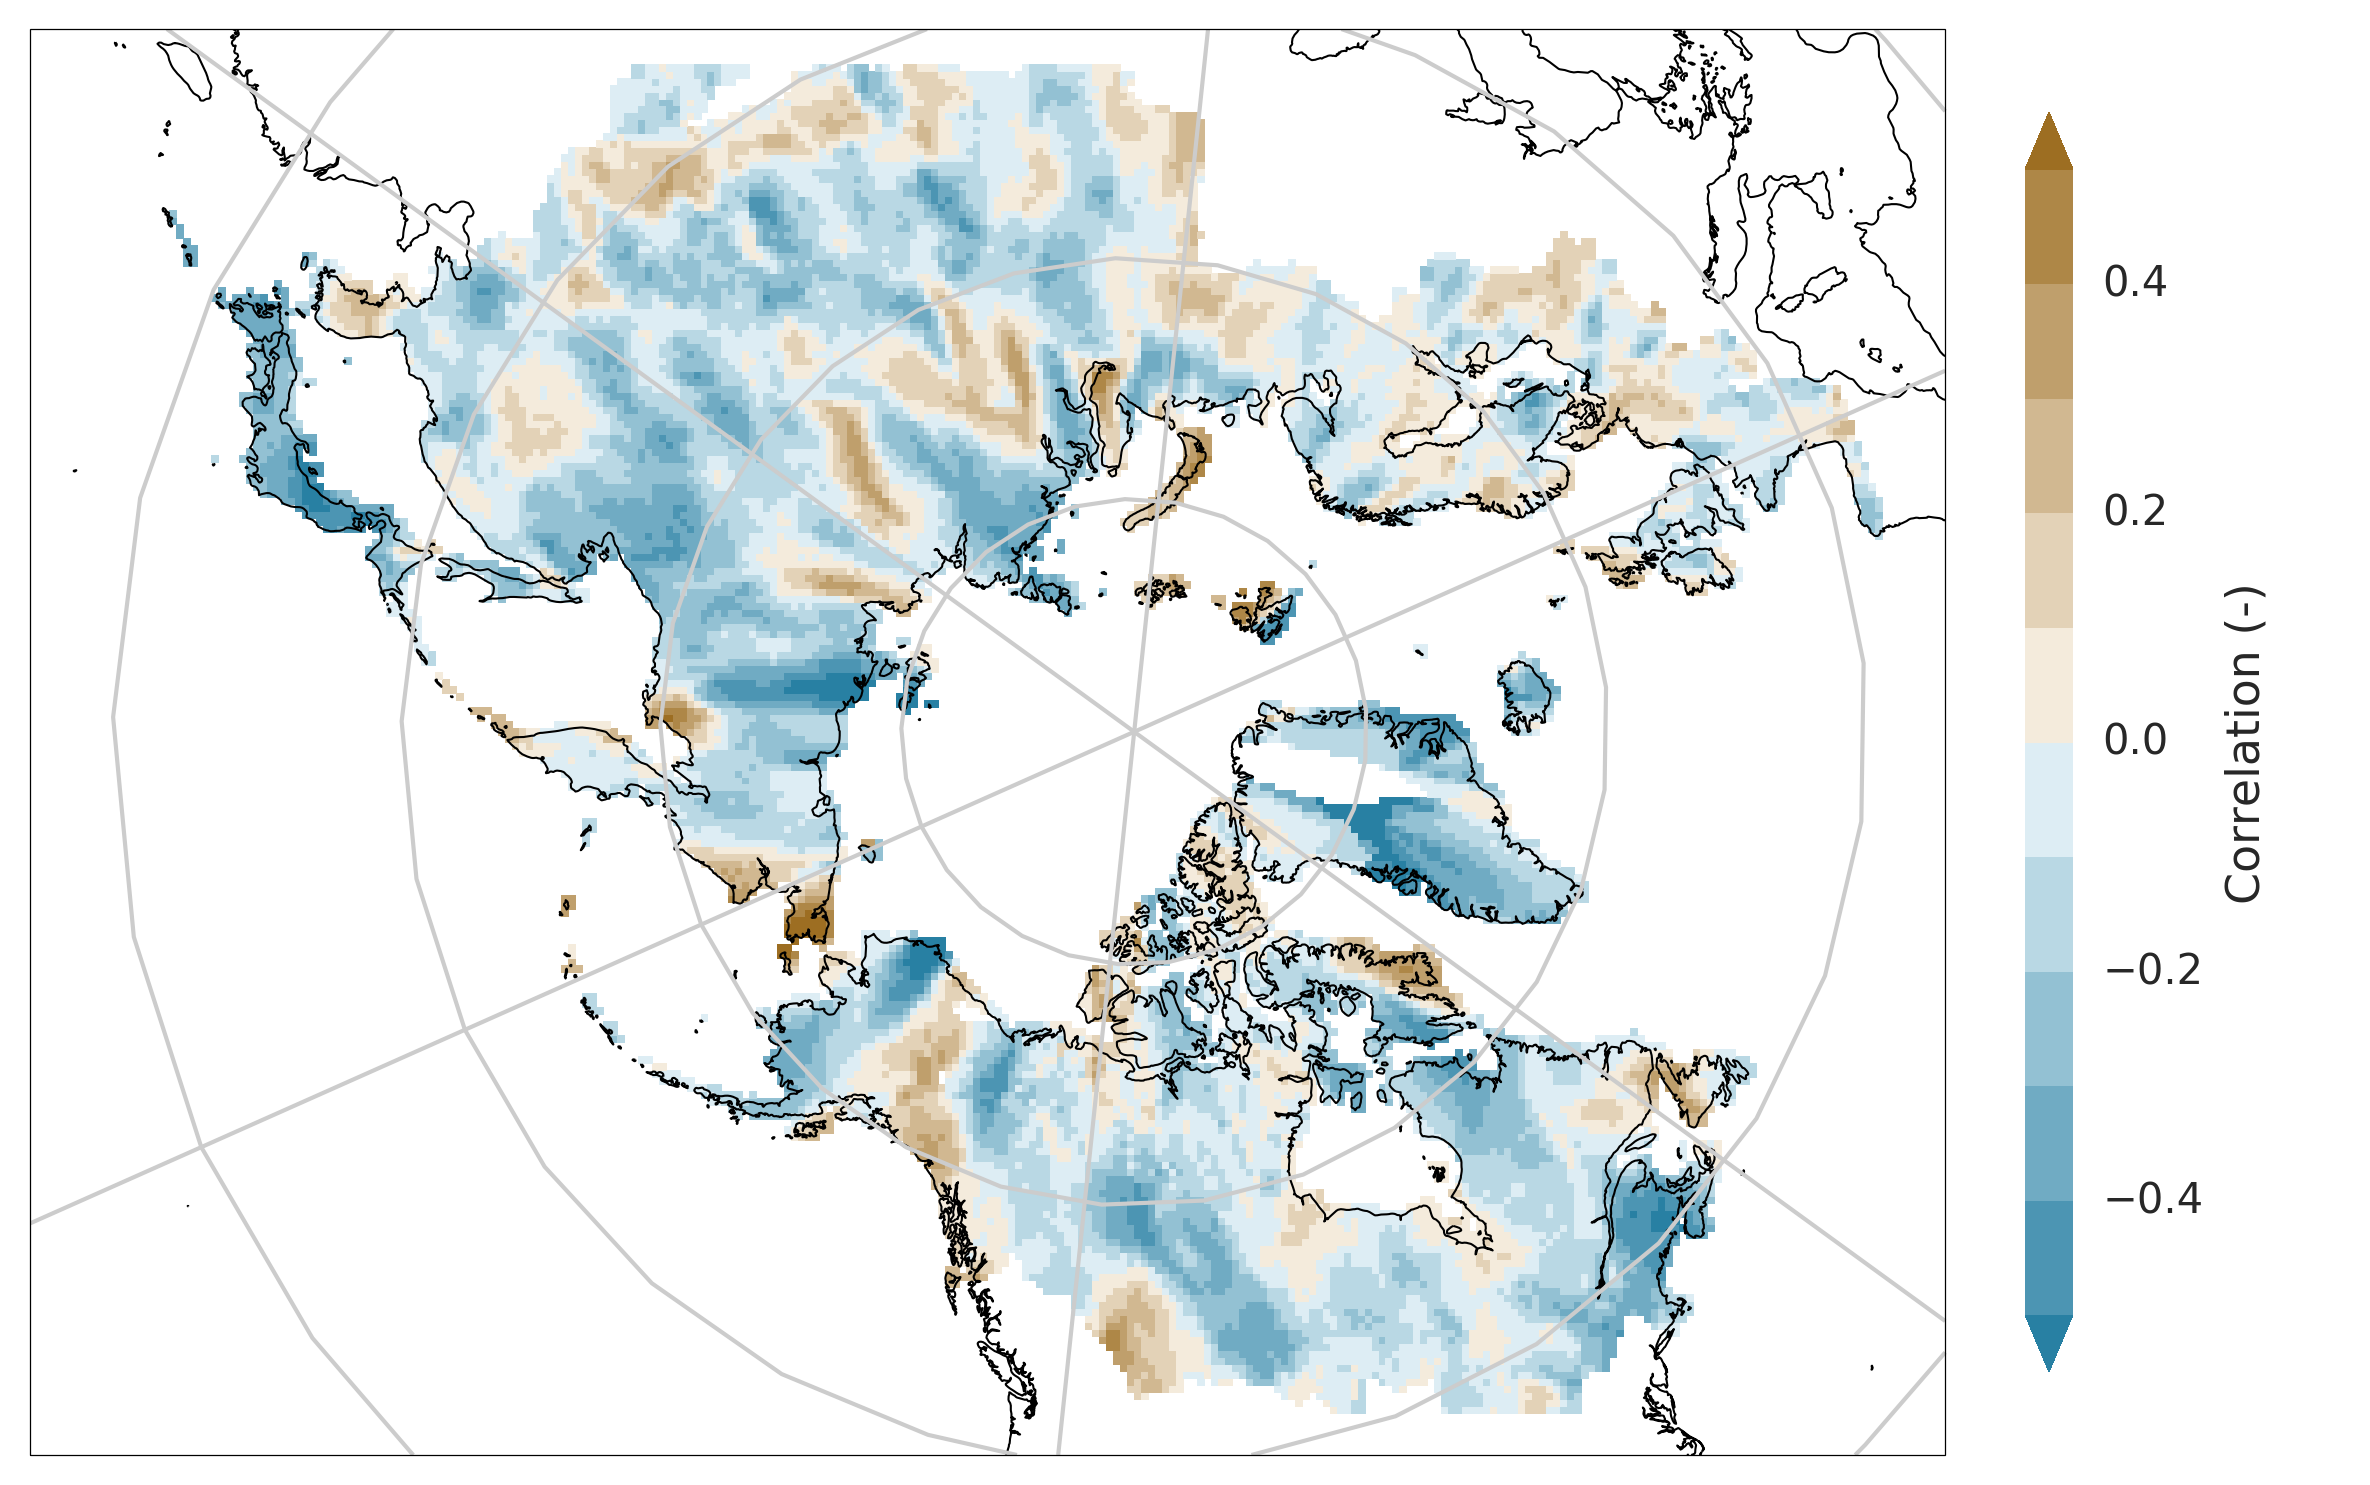
\includegraphics[width=12cm,keepaspectratio]{cru_correlation}
  \caption{Spearman rank-order correlation coefficients between observed minimum annual sea ice extent and gridded Oct-Dec precipitation from CRU. Time period 1980-2015.}
  \label{fig:prec_spatial_corr}
\end{figure}

\subsection{RASM simulations}
\label{sec:rasm_results}

% RASM sea ice sensitivity

% BN: This section needs to be beefed up.

% BN: Include some spatial maps of sea ice extents and delve a bit deeper into the results. Do we have minimum sea ice extents at the right time and in the right years (since we are using reanalysis to drive the simulation I assume so.)
% JH: This will have to be done after we submit the dissertation.
Figure \ref{fig:sea_ice_box} shows box-and-whisker plots of sea ice extent from the three RASM simulations described in Section \ref{sec:data_models_ch5} compared to the NSIDC observation-based estimates.
Compared to $RASM_{CONTROL}$, $RASM_{RSI}$ and $RASM_{RSH}$ have reductions in minimum annual sea ice extents of 16\% and 49\% respectively.
In the fall, these simulations include smaller reductions in mean sea ice cover of 3\% and 11\% respectively.
However, compared to the RASM simulations, the observations of sea ice extent demonstrate significantly more interannual variability.
Individual months can be clearly seen in \ref{fig:sea_ice_box} with the lowest values in each simulation corresponding to Octobers, the middle values corresponding to Novembers, and the highest values corresponding to Decembers.
The RASM simulations have interannual standard deviations for each of these months that are 1.6 to 3.5 times smaller than the observations.
This last point may be an artifact of the processing of the daily NSIDC timeseries and is something that we are currently looking into.
 % BN: Perhaps, but you need to discuss the odd distribution of the RASM simulations. Whereas the observation are somewhat evenly distributed across the full range of extents, the RASM simulations show an odd distribution, which appears tri-modal. They either cluster near the mean/median or near the extremes. This is true for all three simulations, which seems very odd to me. Are you sure nothing went wrong in the processing. I am very suspicious that there is not a single year that falls in large parts of the distribution of extents. As a reviewer this would be a red flag that something is not right. You need to check this figure with Andrew and include a discussion.

 % BN: Don't use "assert", because you can assert whatever you want but that does not make it so. In this case, I would argue that there is something fishy and you need to provide some more analysis. We cannot just say this is good enough. Representing a map with the mean sea ice extent in each state (or from a simulation that is close to the center of each cluster) may provide insight into what is going on.

 % BN: Discuss the combination of the three datasets under the SOM discussions. It is not immediately clear to me why you can do that (or what you gain by doing so)

\begin{figure}
  \centering
  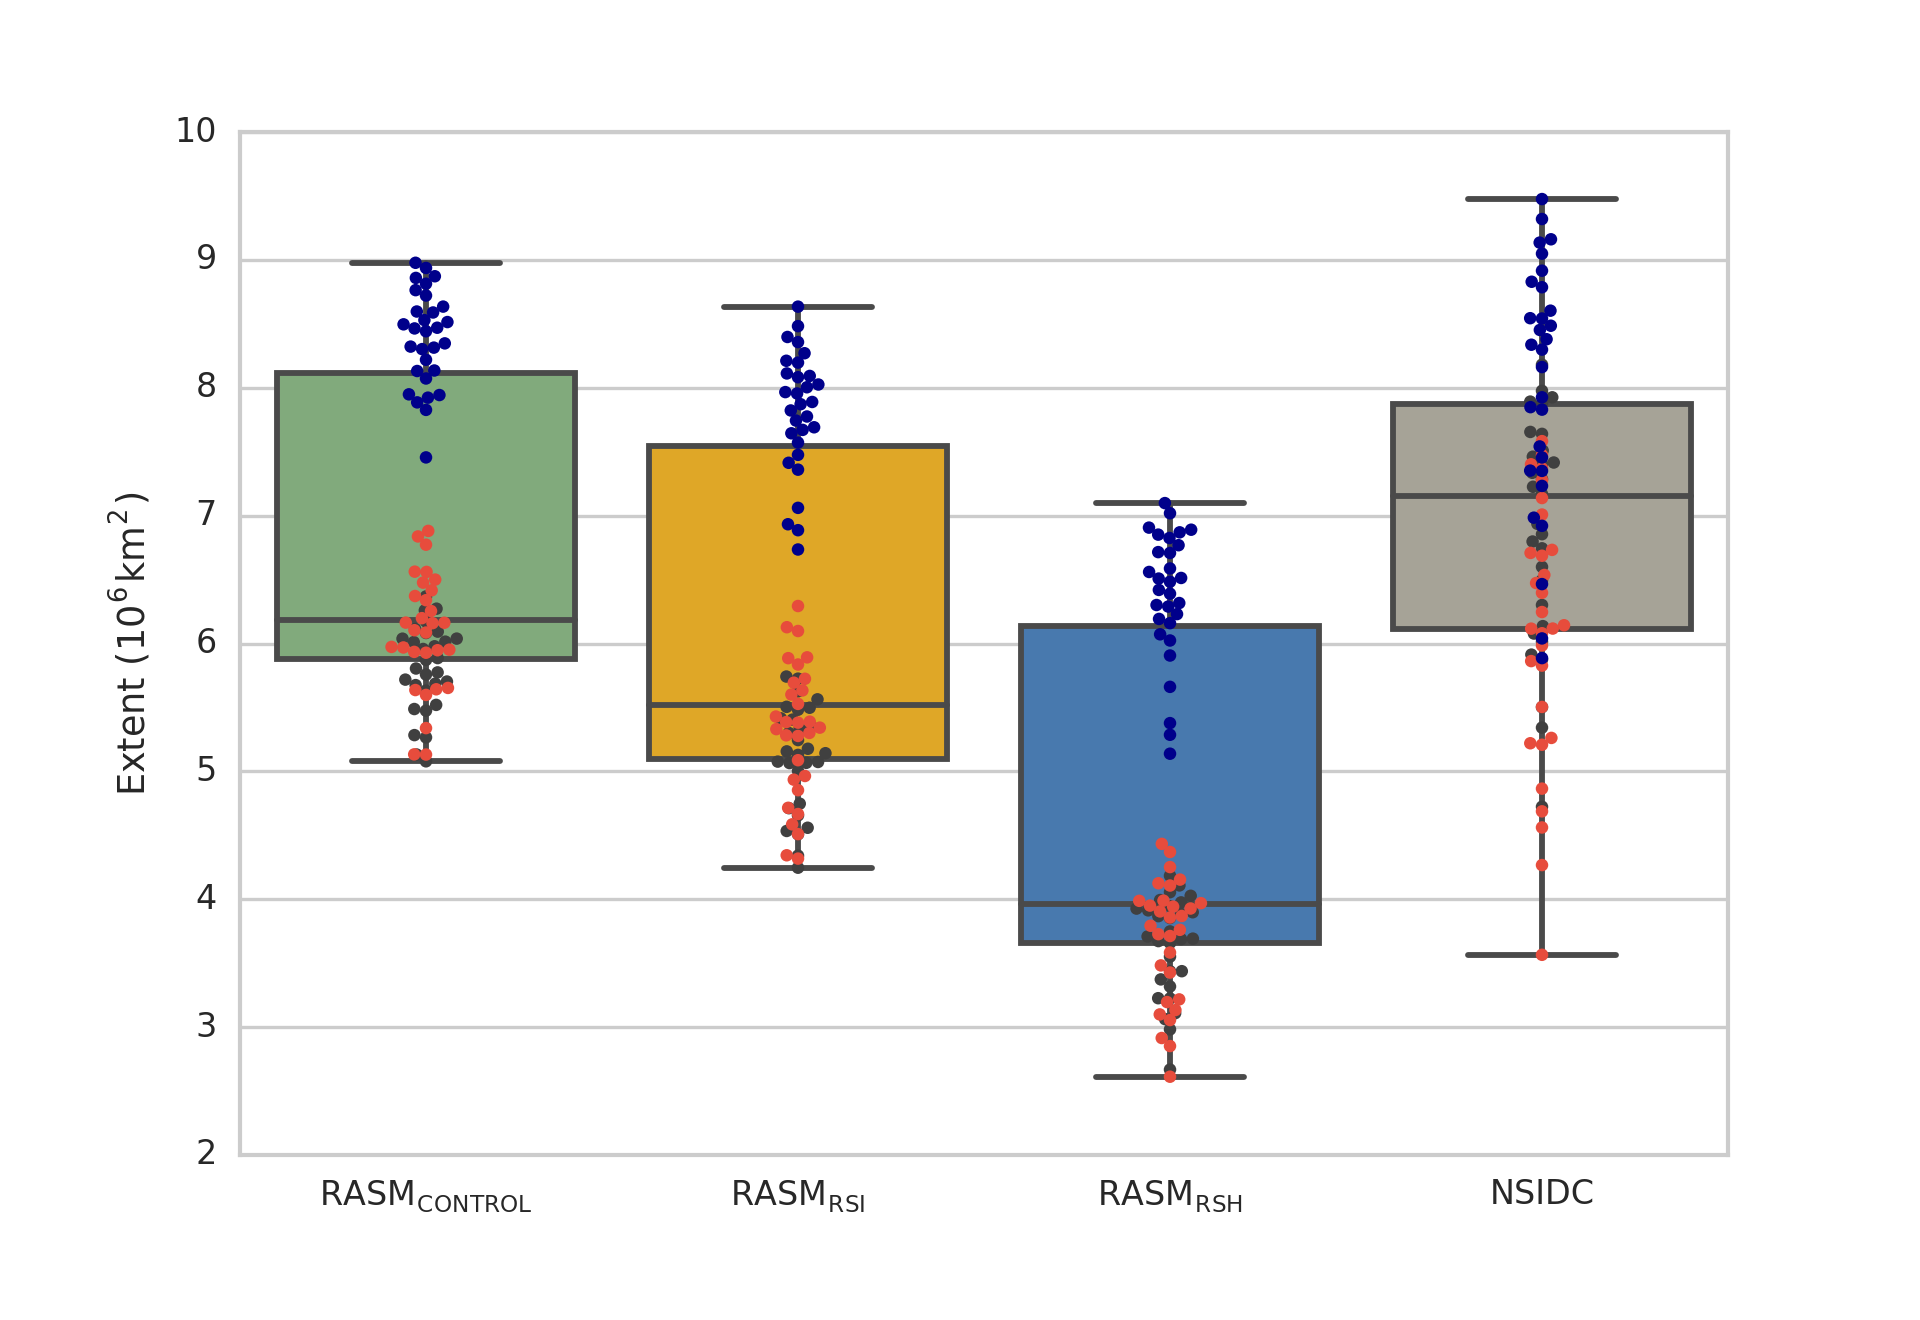
\includegraphics[width=12cm,keepaspectratio]{seaice_boxplots}
  \caption{Distribution of fall (Oct - Dec) sea ice extent in RASM and the NSIDC sea ice index. Time period 1985-2015.}
  \label{fig:sea_ice_box}
\end{figure}

% water budget changes
Figure \ref{fig:fwb} presents the freshwater budget for the three RASM simulations, summarized for the fall months (October-December).
The total moisture convergence for the three simulations are all within 0.05\% of one another, this suggests that changes in .
The reductions in sea ice extent in $RASM_{RSI}$ and $RASM_{RSH}$ are coincident with increases in ocean evaporation of 13\% and 52\%, respectively.
These changes in evaporation from the ocean translate to more modest increases in precipitation over the ocean of 3\% and 11\%.
Associated reductions in convergence over the ocean mask, defined here as P-E between October and December, are found to be 2\% and 10\%. % BN: Is a 2% change meaningful? JH: I'm not sure what you mean.
Finally, while precipitation over land is found to increase relative to the baseline case for both $RASM_{RSI}$ and $RASM_{RSH}$, the increases are relatively small (1\% and 3\% respectively).
These increases in precipitation are sufficient to explain the resulting change in storage (e.g. snow) over land.
Summarizing the water budget, we find that the forced decreases in $RASM_{RSI}$ and $RASM_{RSH}$ lead to significant increases in ocean evaporation but relatively small changes in precipitation over land, despite relatively large changes in ocean evaporation.
Changes in the spatial patterns of precipitation between the three RASM simulations (not shown) lack a regional signal.
While this muted response may be partially explained by the limited interannual variability in the RASM sea ice extent, it also indicates that changes in evaporation from the Arctic Ocean will have to be accompanied with changes in circulation patterns if increases in precipitation are to be attributed to sea ice loss.

\begin{figure}
  \centering
  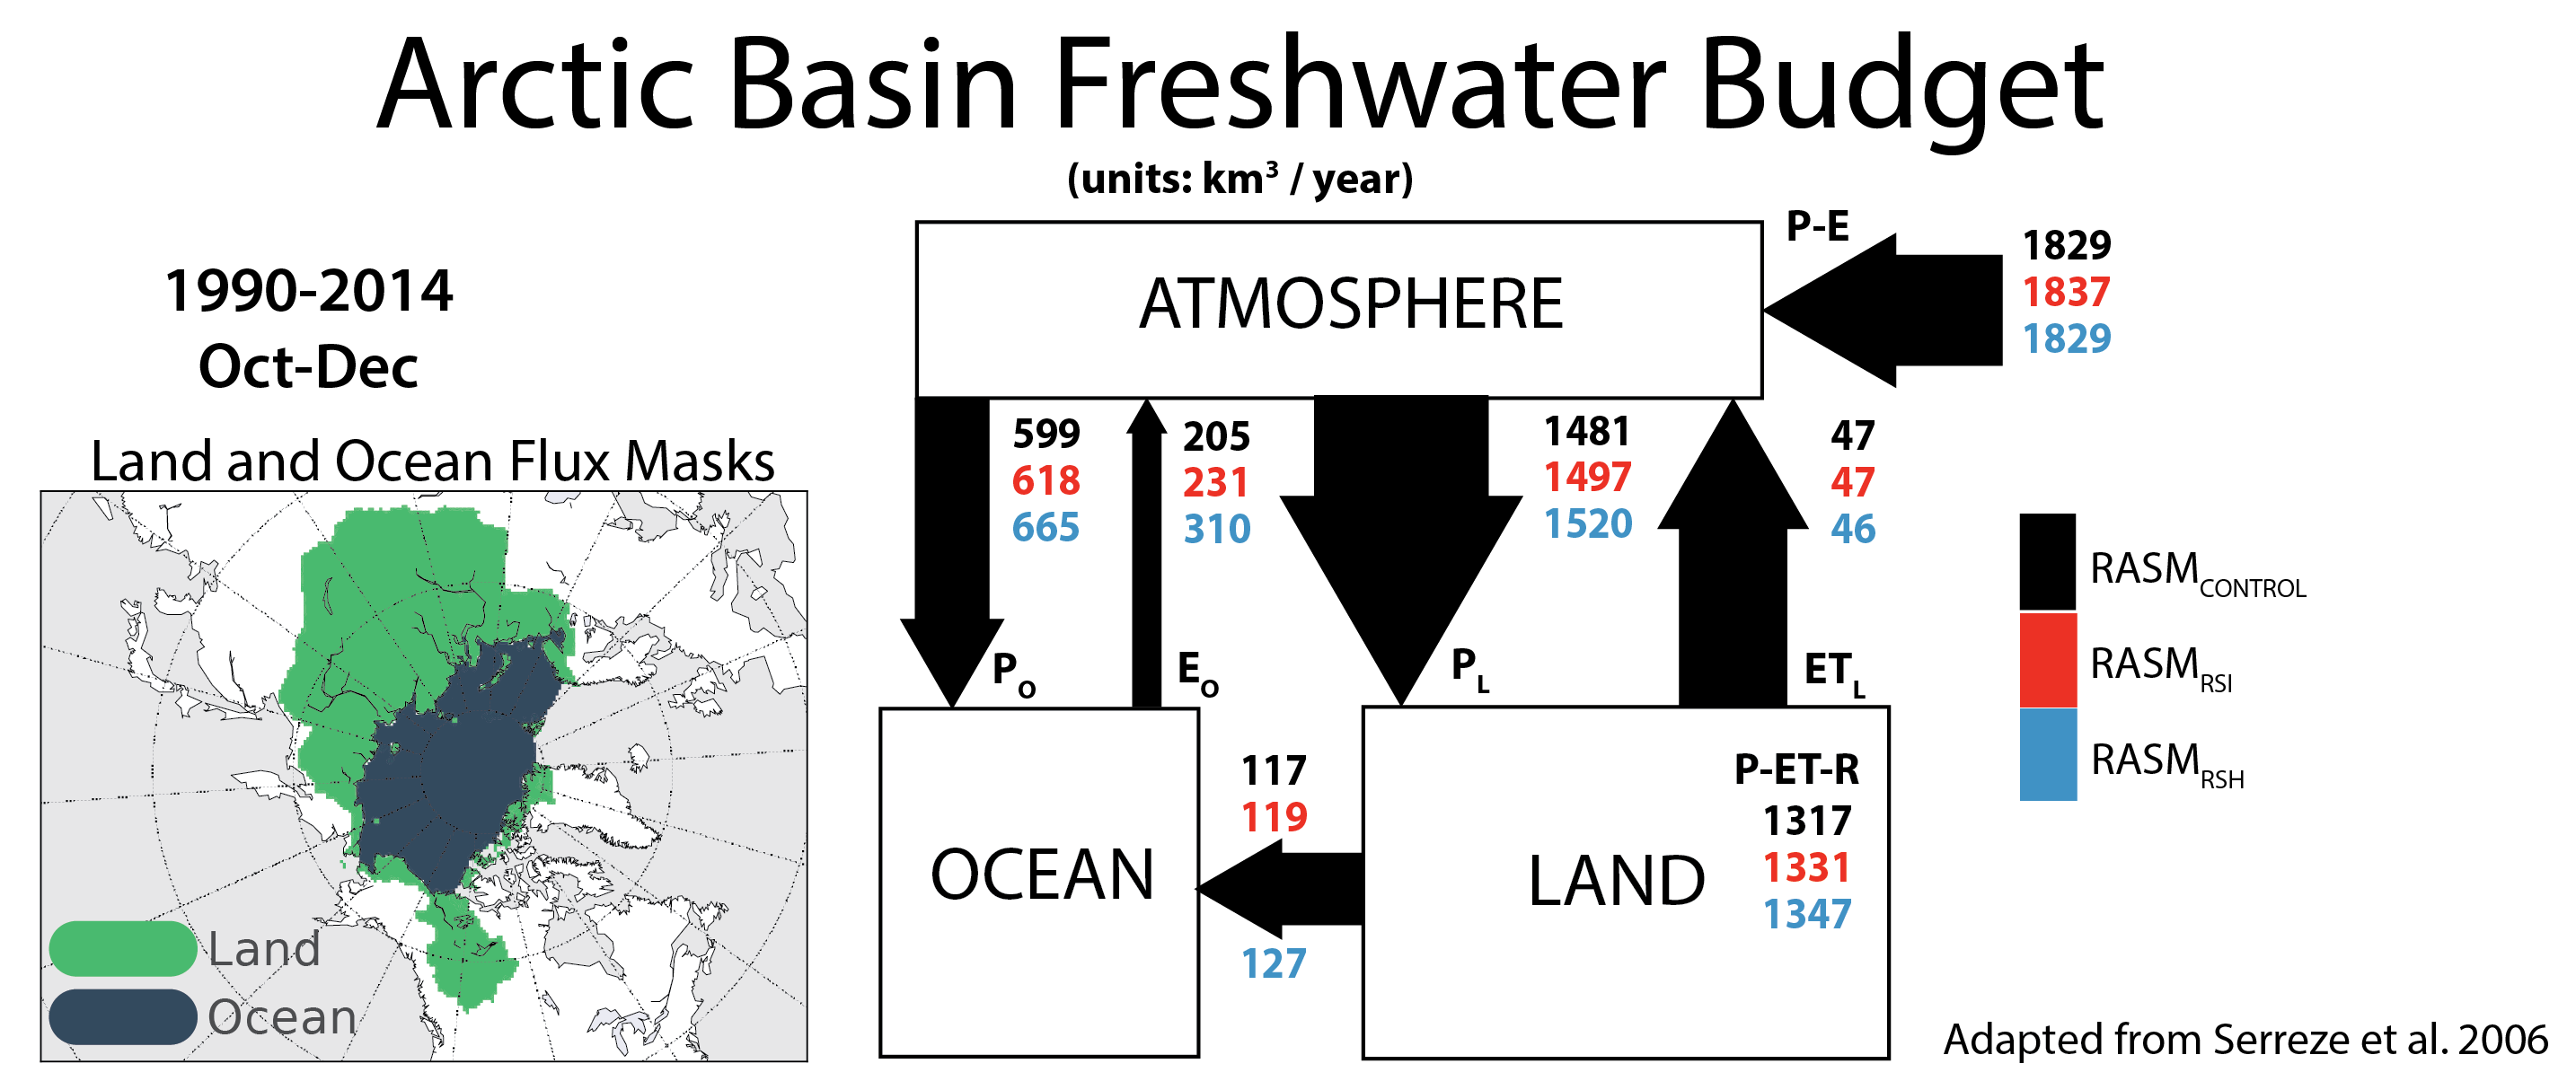
\includegraphics[width=14cm,keepaspectratio]{fresh_water_budget}
  \caption{Arctic freshwater budget, adapted from \citet{Serreze_2006a}.}
  \label{fig:fwb}
\end{figure}

% BN: My main problem with this section is that it reads as if you have found a tool and you are now going to use it just because you have it rather than because you think it may be the best tool for the job. It lacks proper motivation of why you are using SOMs and as a result, the outcomes are rather ambivalent. "I used this technique called SOM and this is what I found". You need to restructure this and provide better motivation for the technique. Rather than being guided by the technique, lead the discussion by what you are interested in (is increased precipitation in the central Arctic a result of a decrease in sea ice extent)? The story is about the latter, not about the technique. Reframing it that way will lead to a better discussion. That starts by removing the "Self-Organizing Maps" as a stand-alone section. It's merely a technique. Focus on the story.
% JH: I've worked to tie the SOM analysis into the story a bit better.

% SOM analysis
We have applied the Self-Organizing Maps technique on standardized evaporation anomalies across the Arctic Ocean to better understand the coupling between ocean sourced evaporation and anomalies in precipitation over land during the fall season.
As we saw in our previous water budget analysis, fairly large relative increases in ocean evaporation led to fairly small changes in precipitation over land.
In applying SOMs, as we do in this section, we will be able to connect regional patterns of ocean evaporation, sea ice, and atmospheric circulation to precipitation patterns over land.

% MASTER SOM
The full, trained Kohonen Layer (or Master SOM) is shown in Figure \ref{fig:master_som}.
The SOM algorithm identified characteristic spatial patterns of evaporation anomalies, with patterns of positive evaporation anomalies toward the top left of Figure \ref{fig:master_som} and patterns of negative evaporation anomalies toward the bottom right.
Here we focus our analysis on four SOM nodes that exhibit the largest hit rate (number of months in a particular pattern) and evaporation patterns of interest: (0,1), (0,3), (1,0), and (1,2).
We will show that the first two SOMs represent generally wet patterns (high precipitation) while the second two represent generally dry patterns (low precipitation) by mapping these patterns to their coincident patterns of precipitation.
In each of these patterns, the combined position, sign, and magnitude of evaporation anomalies in the central Arctic, Kara/Barents sea, and North Atlantic Ocean are characteristically different.

\begin{figure}
  \centering
  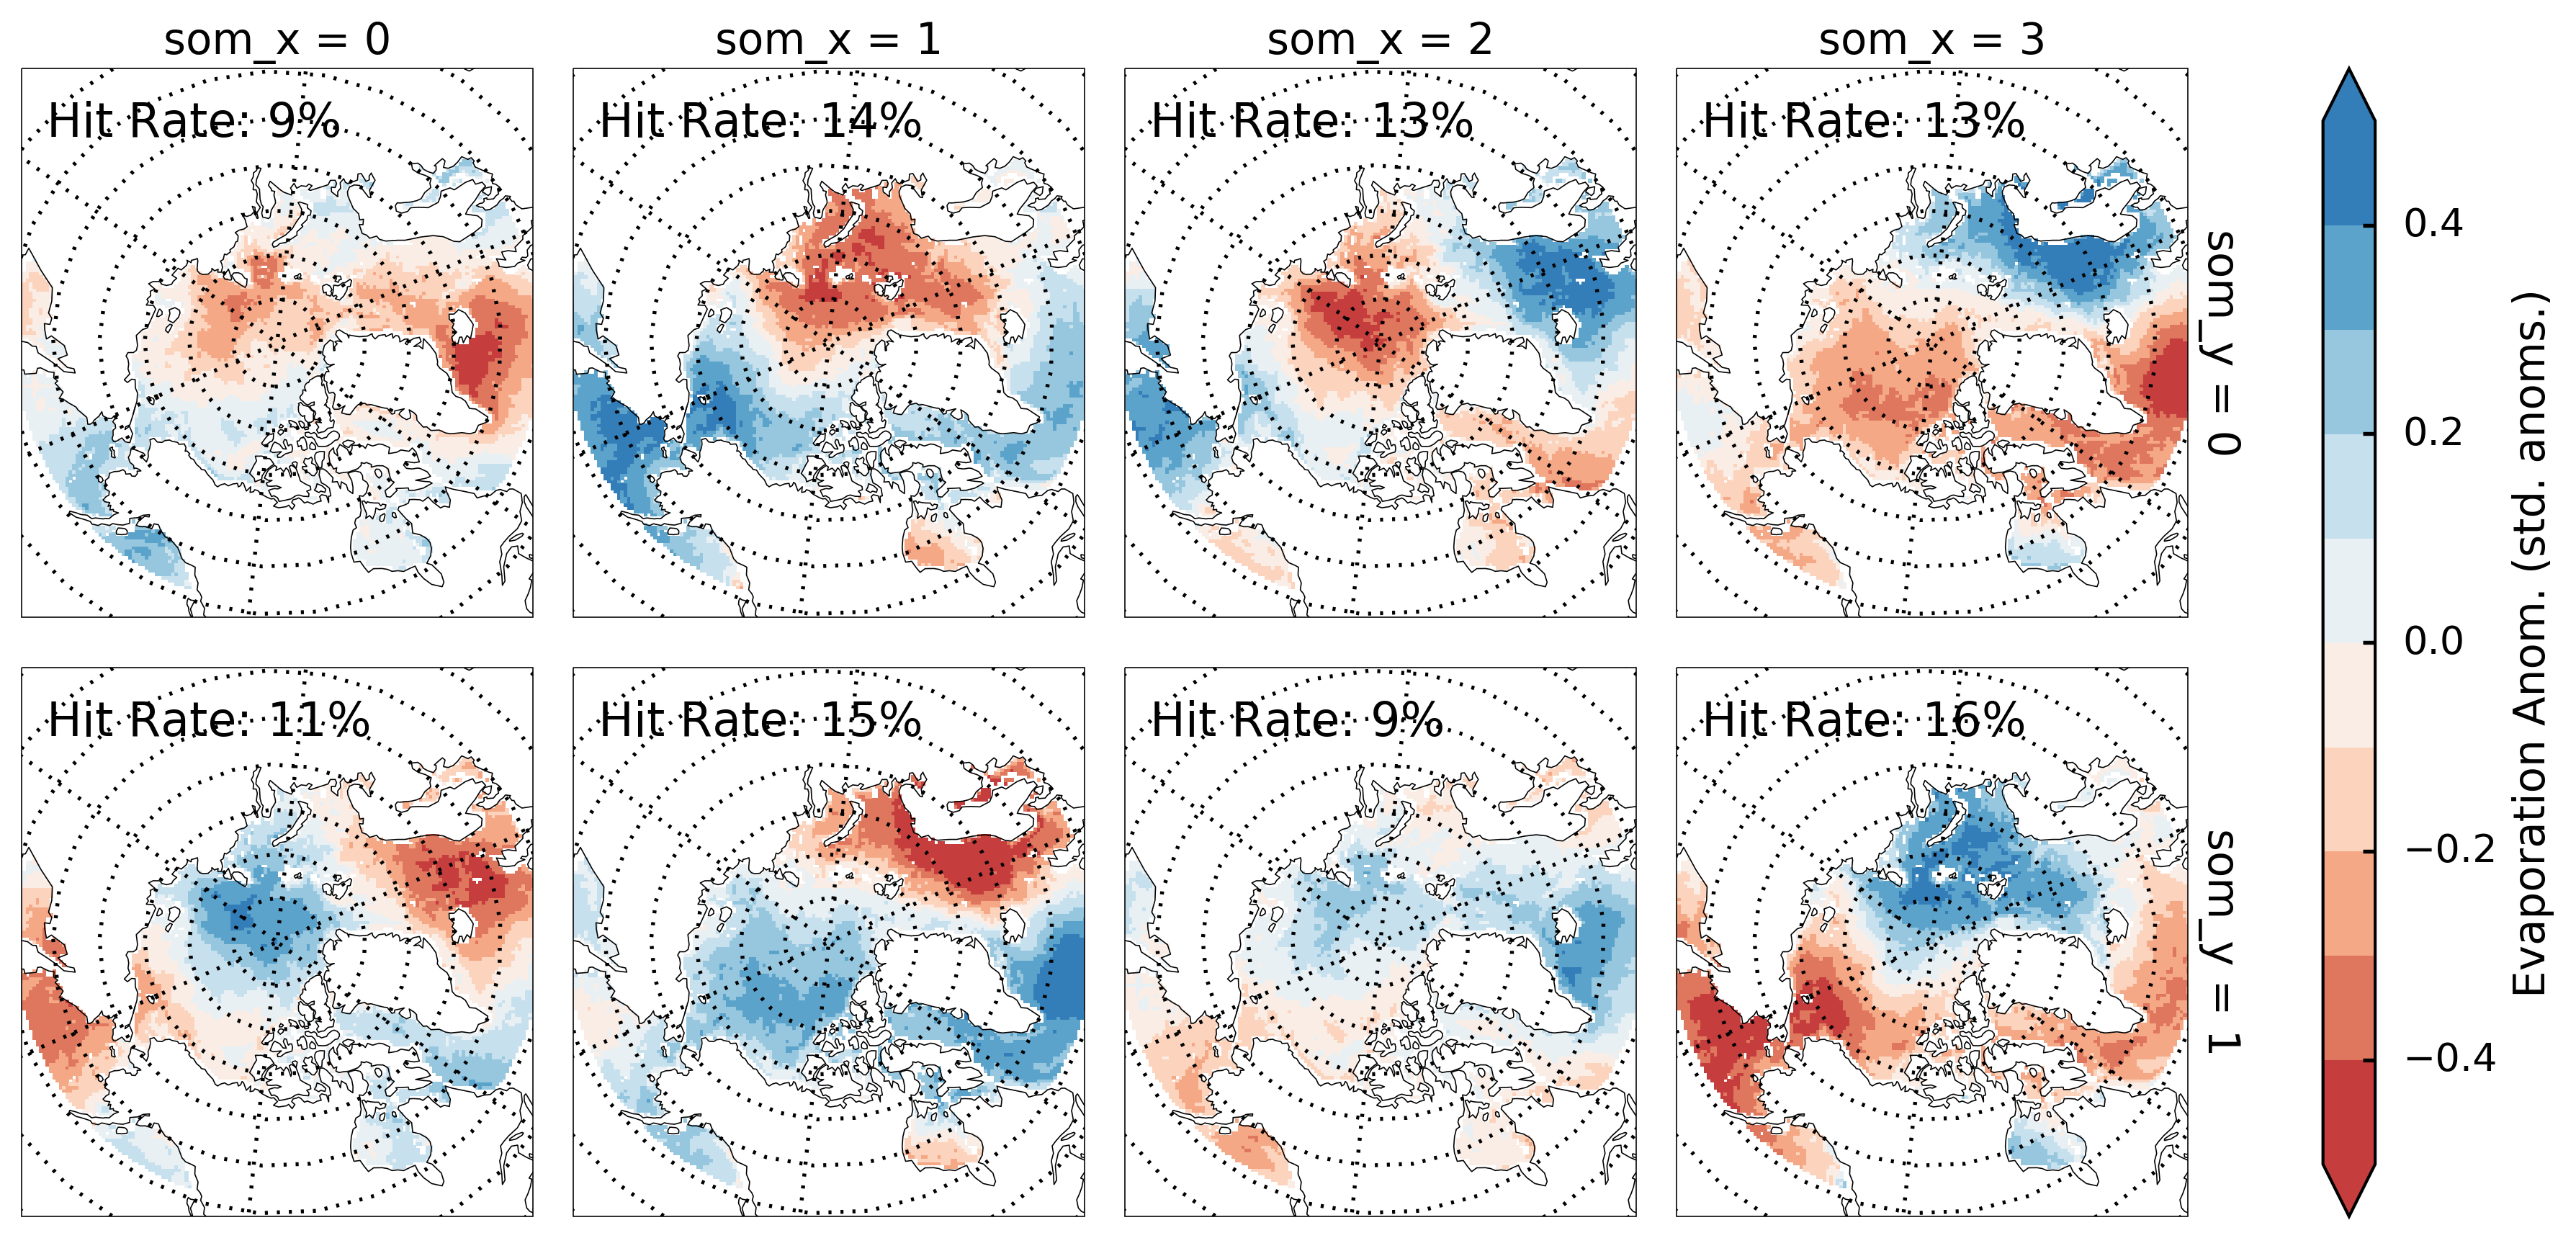
\includegraphics[width=14cm,keepaspectratio]{master_som}
  \caption{Master SOM. The hit rate, shown as the percentage of all the months (270) in the training dataset in each pattern, is shown in the top left corner.}
  \label{fig:master_som}
\end{figure}

% Composite SOM
Figure \ref{fig:composite_som} presents the mapped fields for the four SOM nodes discussed above.
Each of the mapped fields represent the composite mean of all months assigned to SOM node.
Here we focus on ocean evaporation, sea level pressure (SLP), sea ice concentration, precipitation over land, and snow water equivalent.
For node (0,1), anomalously high evaporation rates from the North Atlantic are accompanied by anomalously low pressure in the region.
This combination is found to lead to positive precipitation anomalies over Northern Europe.
Node (0,3) exhibits positive evaporation anomalies in the Kara and Barents Seas and negative evaporation anomalies in the North Atlantic.
SLPs for this node are anomalously high across North America from Alaska to Greenland, indicating a southward shift of the storm track.
Corresponding precipitation anomalies for node (0,3) are positive over eastern Europe and central Siberia.
Neither of the wet nodes have sea ice concentration anomalies that can be clearly tied to evaporation or precipitation anomalies.
The lack of correspondence between sea ice and evaporation anomalies indicates that variability in the fall evaporation flux in RASM is largely being driven by patterns in the ocean and atmosphere.

\begin{figure}
  \centering
  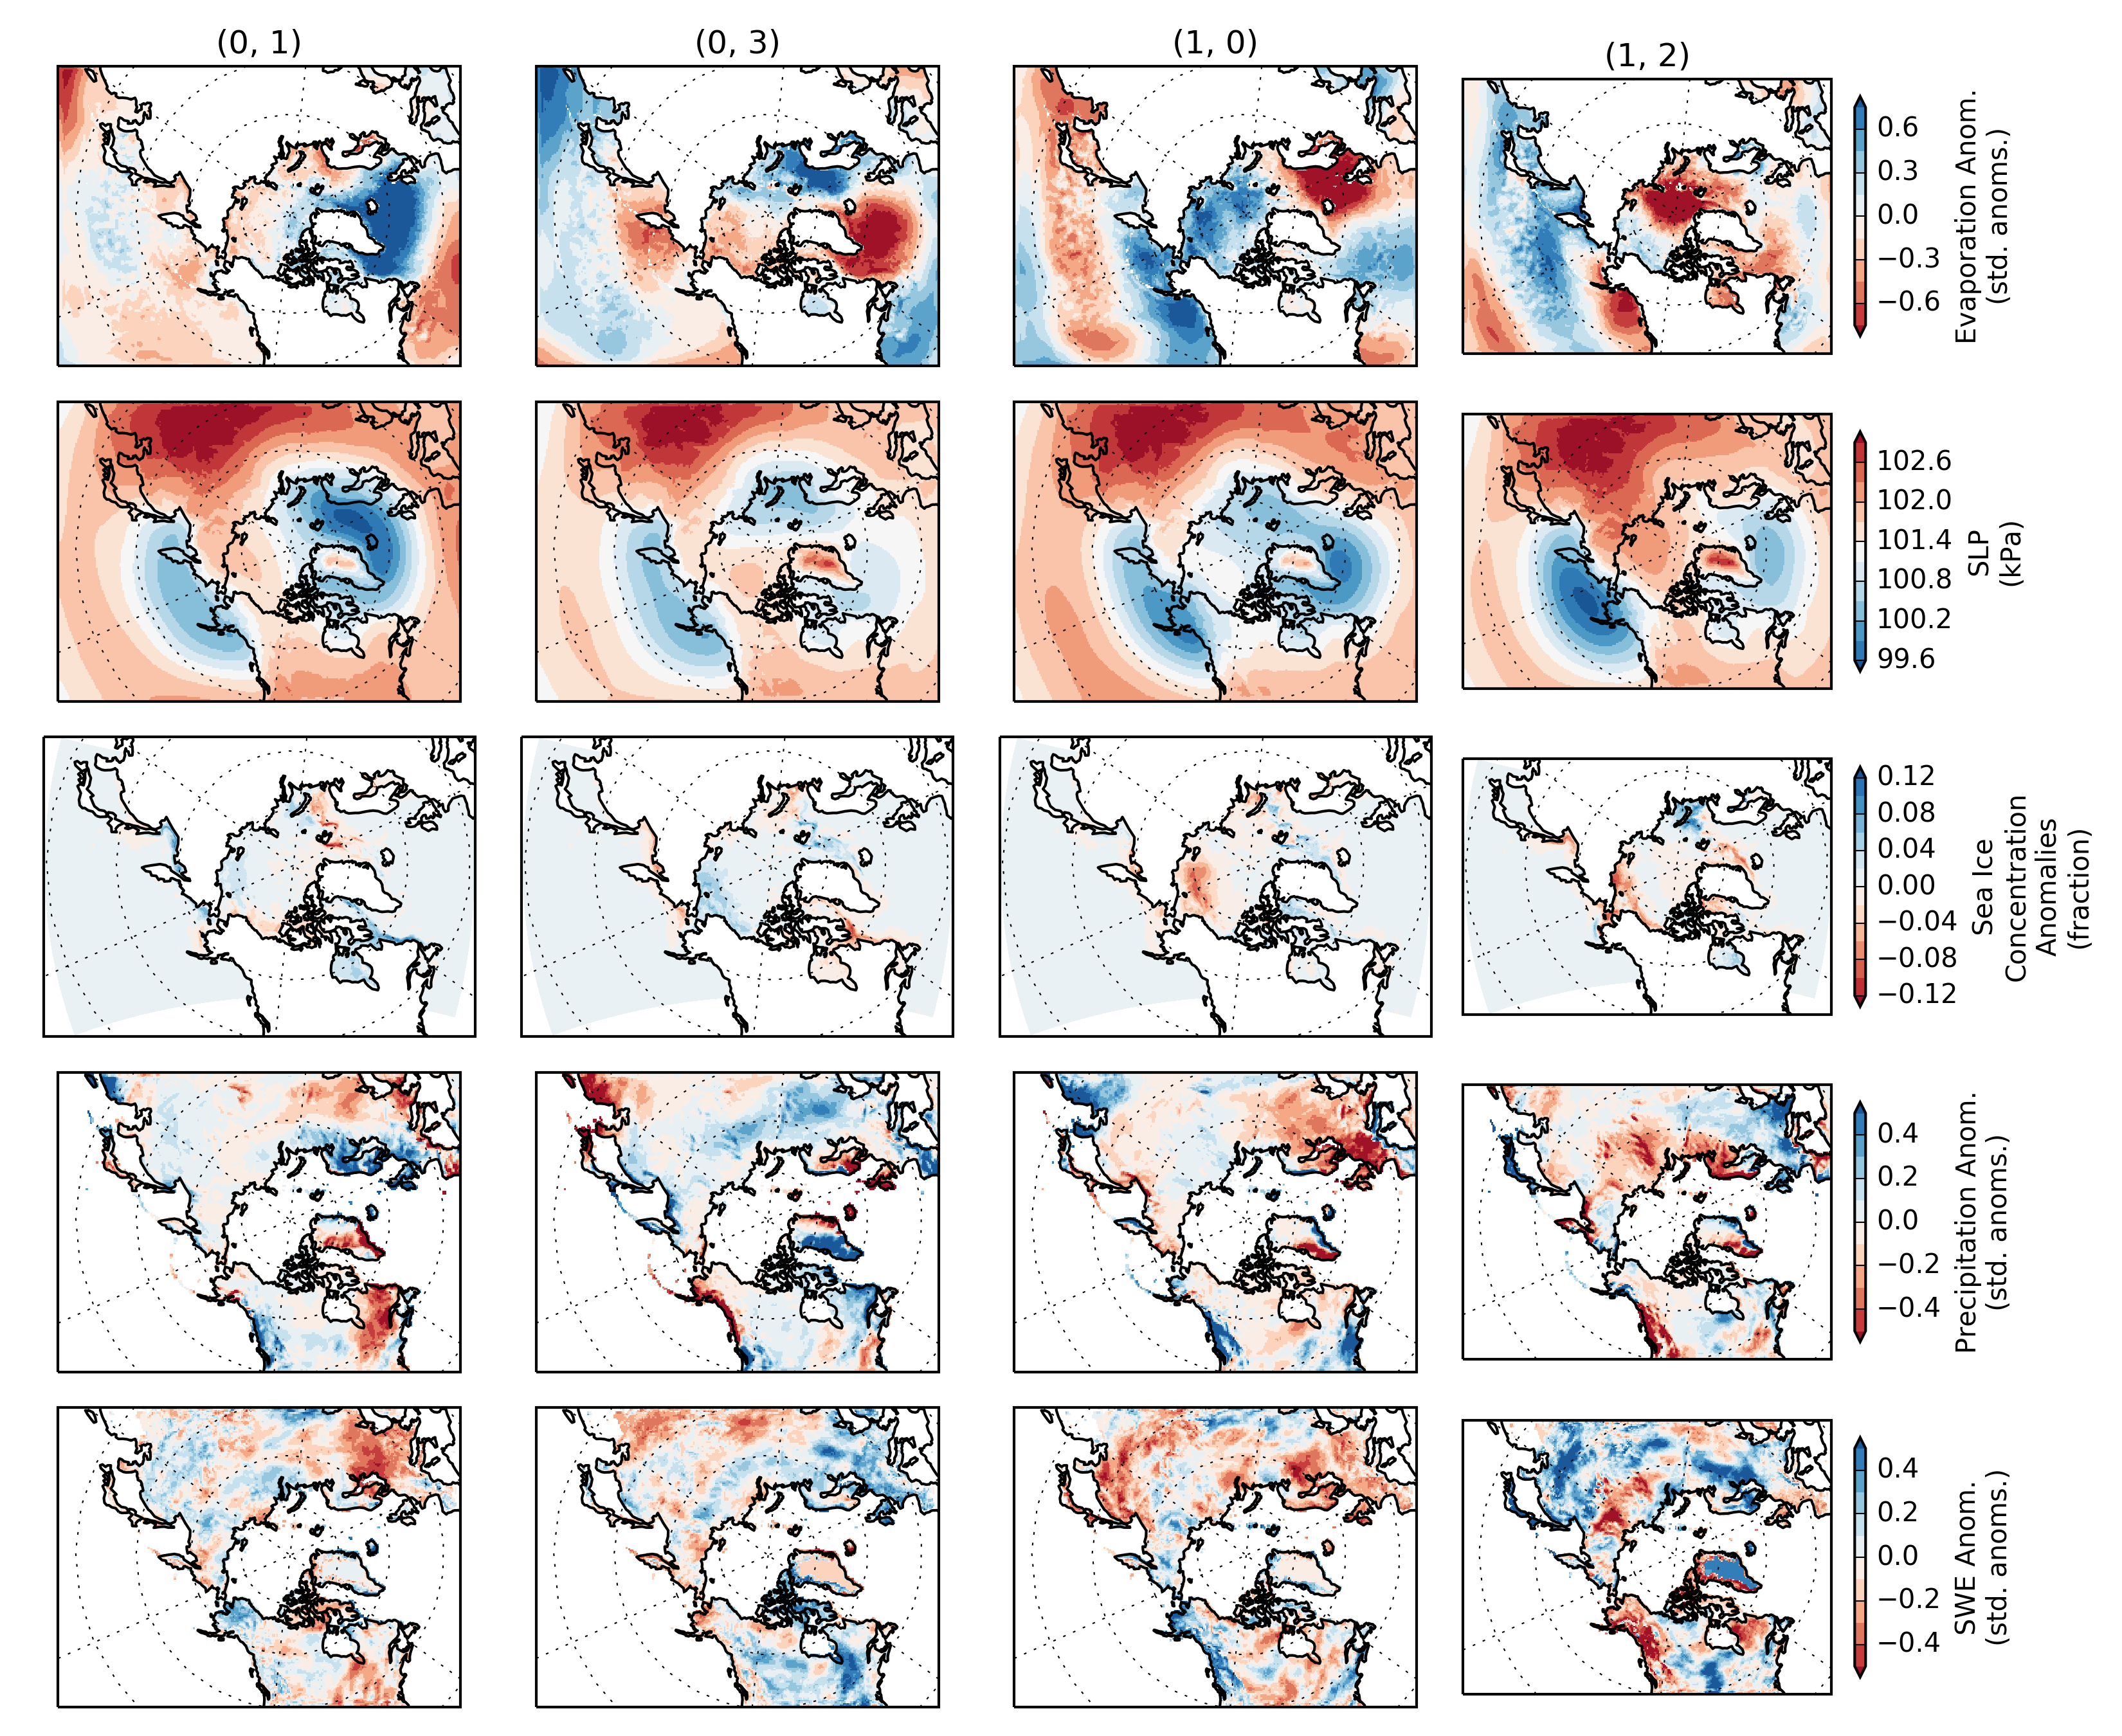
\includegraphics[width=15cm,keepaspectratio]{composite_som}
  \caption{SOM nodes (0,1), (0,3), (1,0), and (1,2) mapped to ocean evaporation, sea level pressure (SLP), sea ice concentration, precipitation over land, and snow water equivalent. Except for sea level pressure, values plotted are the average anomalies across all the members of each node.}
  \label{fig:composite_som}
  % BN: I don't know how to interpret the ET units
  % BN: Should this analysis be limited to the Central Arctic?
\end{figure}
% TODO: get the subplots to align better

The selected dry nodes, (1,0) and (1,2), are characterized by negative evaporation anomalies east and north of Greenland, respectively, and positive anomalies in the central Arctic and Siberian Shelf.
Both nodes are mapped to negative sea ice concentration anomalies along the Siberian Shelf.
In node (1,2), positive sea ice concentration anomalies in the Kara Sea correspond to the negative anomalies ocean evaporation, although the spatial extent is considerable larger in the evaporation anomalies.
Node (1,2) also includes positive SLP anomalies across the central Arctic.

% Hit Map
The trained SOM can be used to identify the frequency of occurrence of each pattern as a function of month (October, November, or December) and RASM simulation ($RASM_{CONTROL}$, $RASM_{RSI}$, or $RASM_{RSH}$).
Figure \ref{fig:som_hit_freq} plots the mapping frequency, by month and simulation, for each node in the 2x4 SOM.
Node (0,1), which has a large region of positive evaporation anomalies across the North Atlantic, occurs nearly twice as frequently in $RASM_{RSH}$ as in $RASM_{CONTROL}$.
The opposite is found in node (0,3), where the hit frequency is found to decrease under reduced sea ice conditions.
Interestingly, the hit frequency for dry nodes [e.g. (1,0) and (1,2)] is mostly stable between the simulations.
On the whole, the SOM analysis indicates that decreasing sea ice extent and the associated evaporation changes are most likely to contribute to wetting trends over land when these changes are accompanied by a shift in atmospheric circulation [e.g. node (0,3)].
Global climate models tend to suggest that future Arctic climate will be stormier \citep{Vavrus_2012} and that winter circulation patters may trend toward a more variable pattern.
However, the fact that the patterns with large shifts in frequency [(0,1) and (1,2)] shift in directions that limit the impact of sea ice loss, indicates that the precipitation response may be dampened.

\begin{figure}
  \centering
  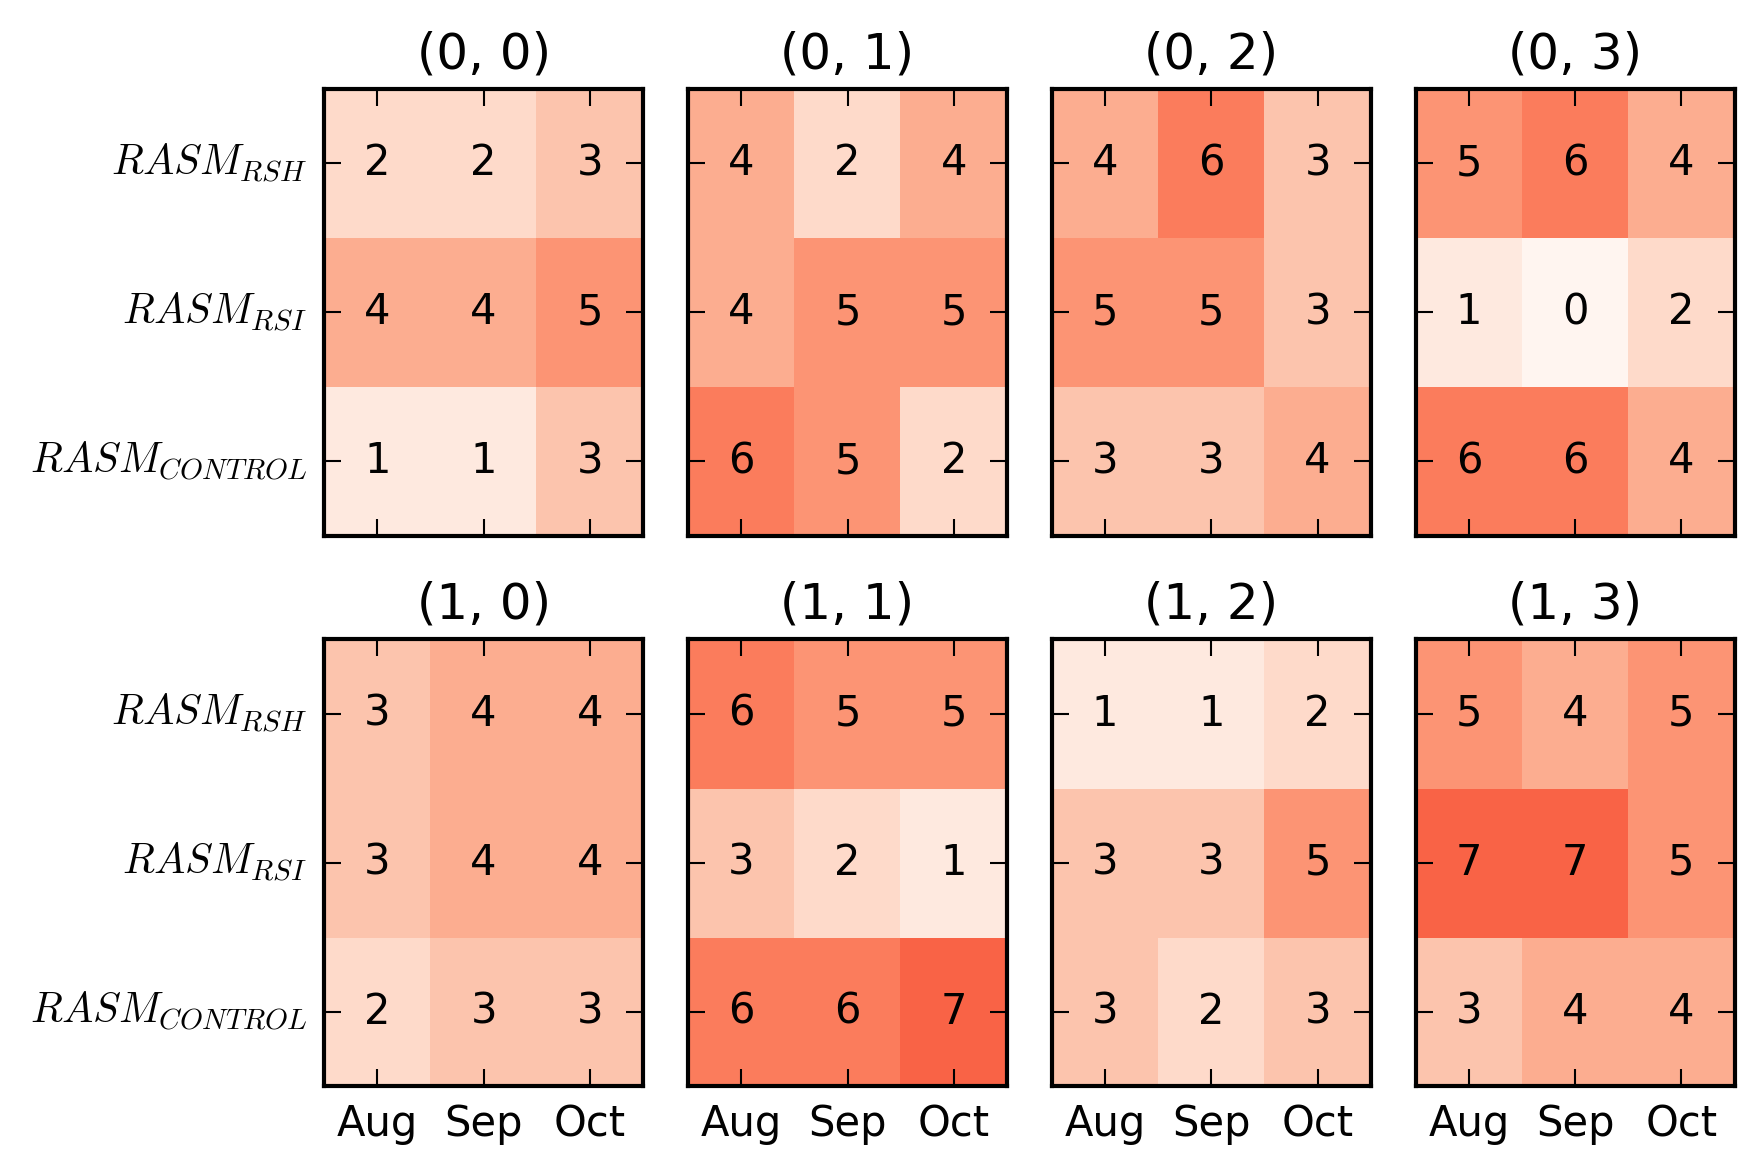
\includegraphics[width=10cm,keepaspectratio]{som_hit_freq}
  \caption{SOM hit frequency by month and RASM simulation.}
  \label{fig:som_hit_freq}
\end{figure}

\section{Conclusions}
\label{sec:conclusions_ch5}

We have investigated the relationship between sea ice extent and early winter precipitation over the Pan Arctic land masses.
We have demonstrated observed interannual covariation between sea ice extent and precipitation over land.
Our initial hypothesis was that variations in sea ice extent were a driving factor in precipitation over land in the fall.
A water budget analysis highlighted that although relatively large changes in winter evaporation from the Arctic Ocean are expected (50\% in our simulation with the lowest sea ice concentration), these changes are proportionally small when compared to the precipitation flux over land.
Furthermore, the modest increases in terrestrial fall season precipitation simulated by RASM under reduced sea ice conditions indicate that there will have to be significant circulation changes in the future if ocean sourced evaporation is likely to significantly impact precipitation over land.
Our SOM analysis has also pointed us in this direction, which is that the ties between evaporation and precipitation are only robust under certain atmospheric circulations.
Across Eurasia, the dominant coupling between precipitation and Arctic Ocean evaporation requires low pressure anomalies over the central Arctic, similar to the negative phase of the Arctic Oscillation \citep{Thompson_1998}.
Previous work by \citet{Cassano_2014}, using partially coupled global simulations with prescribed sea ice, has also indicated that reductions in sea ice extent in the fall may contribute negative sea level pressure anomalies over the Arctic Ocean.

Of particular interest is the sea ice state in the Kara and Barents Seas.
As sea ice declines, we expect that this coupling will become stronger, especially if the Arctic is to become stormier.
We have found that sea ice retreat along the Siberian shelf and north Alaskan coast is holds less influence on precipitation regional patterns.
In these areas, the circulation patterns (low pressure in North Pacific) tend to limit the influence of enhanced evaporation along the retreating ice edge.

\chapter{Conclusions and Recommendations}
\label{chap:conclusions}

\section{Conclusions}
The primary goal of this dissertation was to develop and apply the Regional Arctic System Model (RASM) to better represent and understand key hydroclimatological processes in the Arctic.
This work was motivated by four main research needs: 1) the need to better understand land surface process behavior specific to the Arctic, 2) the need to better understand the coupled interactions between the high-latitude land surface and the other core physical climate components, 3) the need to better understand how changes in the global climate system will manifest in the Arctic, and 4) the need to improve model capacity for process representation and prediction.

The development of RASM attempts to address these gaps.
As a regional model, RASM inherently includes fewer degrees of freedom than a global model would \citep[e.g. ][]{Deser_2016}, as it is limited by its specified horizontal boundary conditions.
While this fact limits RASM's applicability in studies of global scale, it uniquely positions RASM as a tool for addressing questions regarding regional processes.
RASM is also computationally less expensive than global models would be if run at the same temporal and spatial resolutions.
This has proven to be immensely useful in the development of RASM as it has allowed for numerous iterations of model versions.
The combination of these two points supports RASM's use as a testbed for high-resolution coupled model development.

This dissertation was made up of three core chapters.
The first two focused on the development and evaluation of the land surface (Chapter \ref{chap:land_surface}) and streamflow routing (Chapter \ref{chap:streamflow}) model components within RASM.
In Chapter \ref{chap:fall_prec}, RASM was used to evaluate how changes in sea ice cover in the Arctic Ocean impacted precipitation patterns over land.

In Chapter \ref{chap:land_surface}, we introduced a novel coupling of the Variable Infiltration Capacity (VIC) model within RASM.
We evaluated how RASM compared to a range of observations, including in situ measurements of turbulent fluxes and streamflow, gridded climatological datasets of precipitation and temperature, and remote sensing estimates of snow and surface albedo.
We also compared the performance of RASM's land surface model with the ERA-Interim and MERRA global reanalysis models, identifying the largest differences in the partitioning of turbulent heat fluxes.
Our comparisons identified areas where VIC was performing better than these reanalyses, such as in the partitioning of precipitation into streamflow and evapotranspiration.
We also identified areas where the representation of the land surface in VIC and RASM could be improved, such as the representation of soil thermal and canopy processes, motivating ongoing development on the land, atmosphere, and streamflow routing model components.

We introduced a new river routing scheme (RVIC) for coupled climate models in Chapter \ref{chap:streamflow}.
In this chapter, we evaluated streamflow simulated by RVIC in RASM against in situ observations and other model based datasets, characterizing the sources of biases in the RASM streamflow flux.
We illustrated the impact streamflow has on the coupled ice-ocean system using two coupled RASM simulations, one with the streamflow flux delivered to the ocean, the other without.
Associated with this chapter is a new coastal streamflow dataset for ocean modeling applications.
This dataset is of higher spatial and temporal resolution than existing datasets used by the ocean modeling community, and provides substantial improvement in the representation of coastal streamflow in ungauged areas such as Greenland and the Canadian Archipelago.

Chapter \ref{chap:fall_prec} applied RASM to better understand how fall precipitation may change given reductions in sea ice cover.
Motivating this chapter was an observation based correlation analysis that indicated that minimum annual sea ice extent and fall season precipitation (August - October) were inversely correlated across most of the pan-Arctic land areas.
In this chapter, we evaluated three RASM simulations, with varying levels of sea ice extent, testing the hypothesis that the observed correlations between sea ice extent and high latitude precipitation are related to anomalous patterns in ocean evaporation and sea ice extent in the fall season.
A water budget analysis for the central Arctic Ocean and surrounding land mass indicated that relatively small decreases in RASM-simulated fall season sea ice extent (3\% and 11\%) can lead to increases in evaporation from the Ocean as high 50\%.
However, we show that changes in precipitation are much smaller (1-3\%).
Finally, using a machine learning technique for pattern recognition, we show that the strongest coupling between sea ice and terrestrial precipitation patterns occurs when there is anomalously high ocean sourced evaporation in the Kara and Barents Sea accompanied by a northeastward shift of the Icelandic Low.

Chapters \ref{chap:land_surface} and \ref{chap:streamflow} were principally model development chapters.
While working on this dissertation, I developed the RVIC streamflow routing model \citep[see also \ref{sec:rvic_dev} ;][]{Hamman_2015,Hamman_2016b} and participated as a core development member of the VIC model \citep[see also \ref{sec:vic_dev}]{Hamman_2016c,Hamman_2016d}.
While the majority of this work extended existing models or reapplied existing algorithms, my contribution focused on implementing new features as well as improving model extensibility and reproducibility.
While the majority of the ideas that made up the models in chapter \ref{chap:land_surface} and \ref{chap:streamflow} were not new, their application in RASM required extensive effort, both in terms of software infrastructure and model tuning and enabled new model experiments.
Furthermore, the evaluation of these models required the development of unique methods for comparing datasets derived from observations and models with the underlying objective of understanding and improving the model.

\section{Recommendations}
The development of RASM version 1.0 has enabled many new scientific opportunities.
Each of the three core chapters in this dissertation exemplify ways that RASM can be used in the future.
Chapter \ref{chap:land_surface} is an example of how RASM can be used as a testbed for improved model performance of individual component couplings.
This chapter discusses specific examples of how, during the development of RASM version 1.0, we implemented new approaches to improve the representation of the land surface in RASM.
Chapter \ref{chap:streamflow} is an example of how RASM can be used to evaluate the impact that an additional process representation (e.g. streamflow) can have in a coupled model.
Chapter \ref{chap:streamflow} demonstrates how RASM may be used for dataset development, providing improved forcing data for uncoupled model applications.
Finally, Chapter \ref{chap:fall_prec} provides an example of how RASM can be used to test the sensitivity of coupled processes at a regional scale, apart from global feedbacks.

Both RASM and VIC continue to be actively developed.
Further development of the VIC land surface scheme has been enabled by the recent release of VIC version 5.0 \citep[see also \ref{sec:vic_dev}][]{Hamman_2016c,Hamman_2016d}.
The incorporation of this updated version of VIC within RASM will allow for improved representation of soil thermal processes (e.g. permafrost), canopy-atmosphere interactions, and blowing snow.
The application and evaluation of RASM at higher spatial resolutions is also an important next step in the development of the project.
Eight years ago, when the RASM project began, 50 km spatial resolution was relatively high for a regional climate model and about 2-4 times higher resolution than typical global models.
In the years since, global models have steadily increased their resolution with many CMIP5 models using 1 degree spatial resolution (111 km at the equator, less in the Arctic).
Future development should focus on making RASM truly stand out as a high-resolution regional model by increasing spatial resolution to 10-25 km.


\printendnotes

% ==========   Bibliography
\nocite{*}   % include everything in the uwthesis.bib file
% \bibliographystyle{plain}
\bibliographystyle{uwthesis}
\bibliography{uwthesis}

% ==========   Appendices
\appendix
\raggedbottom\sloppy
\chapter{The Land Surface Climate in the Regional Arctic System Model - Supplemental Materials}
\label{chap:land_surface_sup}

This appendix includes the supplemental materials from chapter \ref{chap:land_surface}.
This material has been published in its current form in the \textit{Journal of Climate}.
\textcopyright American Meteorological Society.
Used with permission.
\begin{itemize}
    \item \bibentry{Hamman_2016a}.
\end{itemize}

\section{Figures}

\begin{figure}
    \centering
    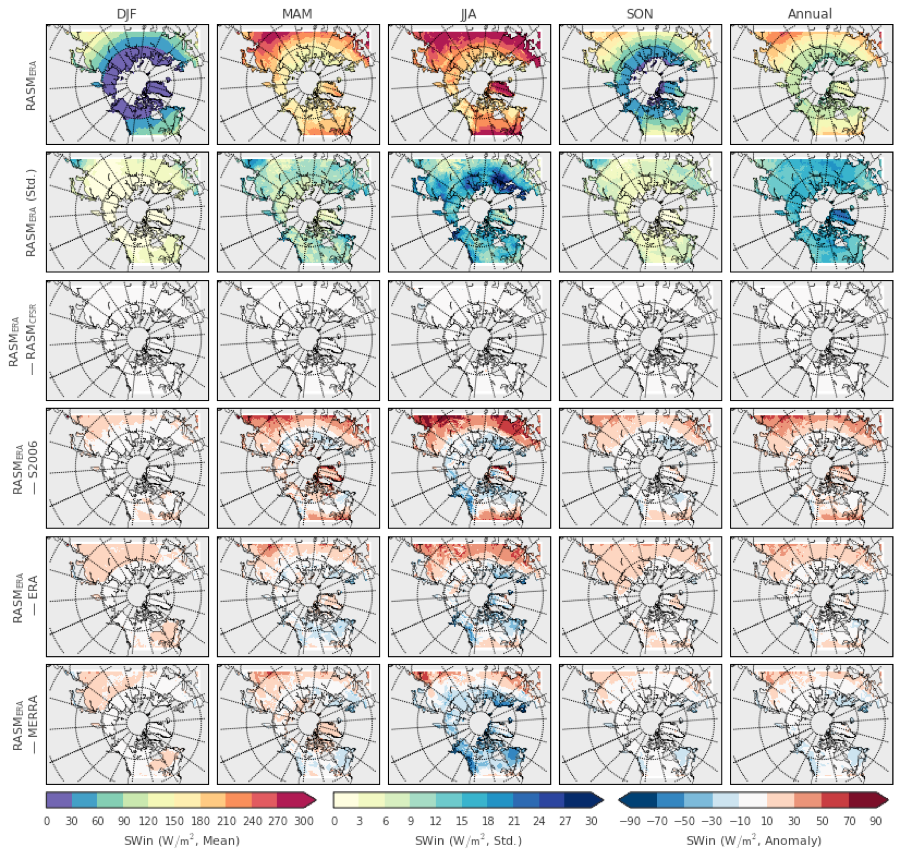
\includegraphics[width=12cm,keepaspectratio]{ch3_S1}
    \caption{Seasonal and annual average downward shortwave radiation (SWin).
    Time period: Sep. 1989 – Aug. 2014.}
\end{figure}

\begin{figure}
    \centering
    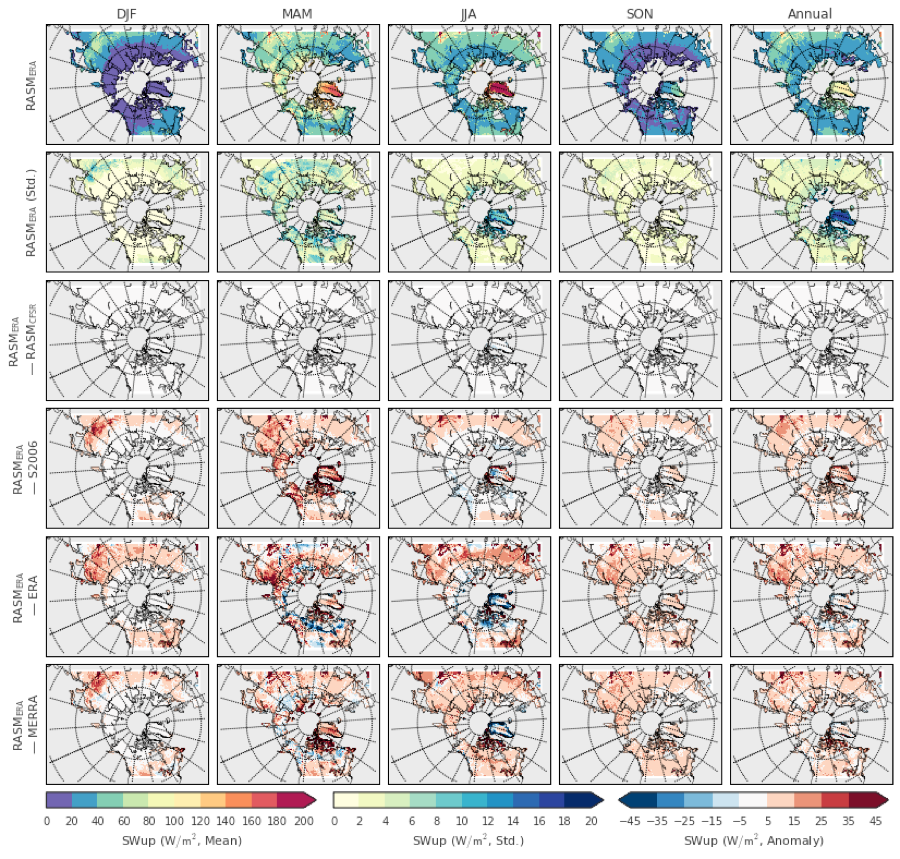
\includegraphics[width=12cm,keepaspectratio]{ch3_S2}
    \caption{Seasonal and annual average upward (reflected) shortwave radiation (SWup).
    Time period: Sep. 1989 – Aug. 2014.}
\end{figure}

\begin{figure}
    \centering
    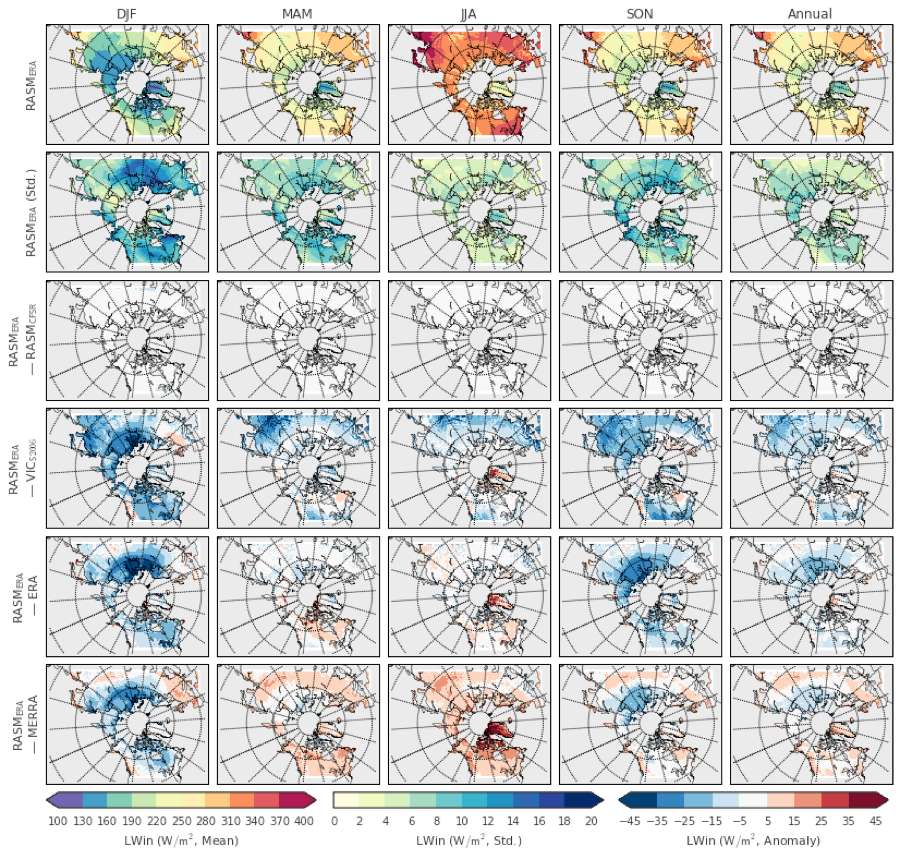
\includegraphics[width=12cm,keepaspectratio]{ch3_S3}
    \caption{Seasonal and annual average downward longwave radiation (LWin).
    Time period: Sep. 1989 – Aug. 2014.}
\end{figure}

\begin{figure}
    \centering
    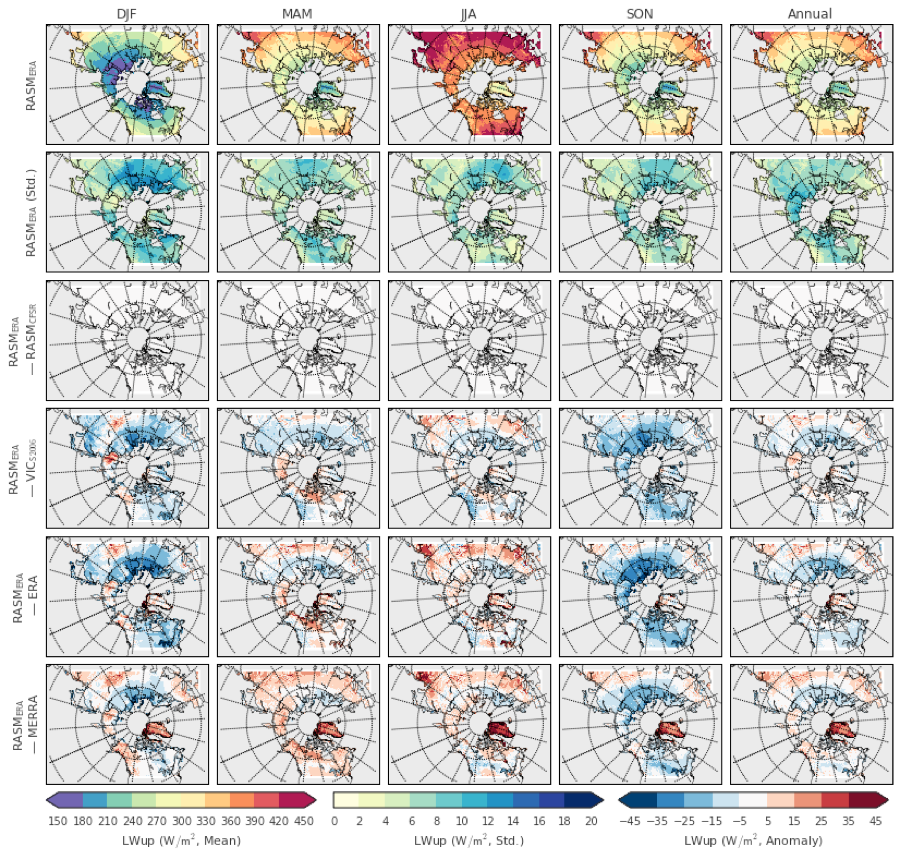
\includegraphics[width=12cm,keepaspectratio]{ch3_S4}
    \caption{Seasonal and annual average upward longwave radiation (LWup).
    Time period: Sep. 1989 – Aug. 2014.}
\end{figure}

\begin{figure}
    \centering
    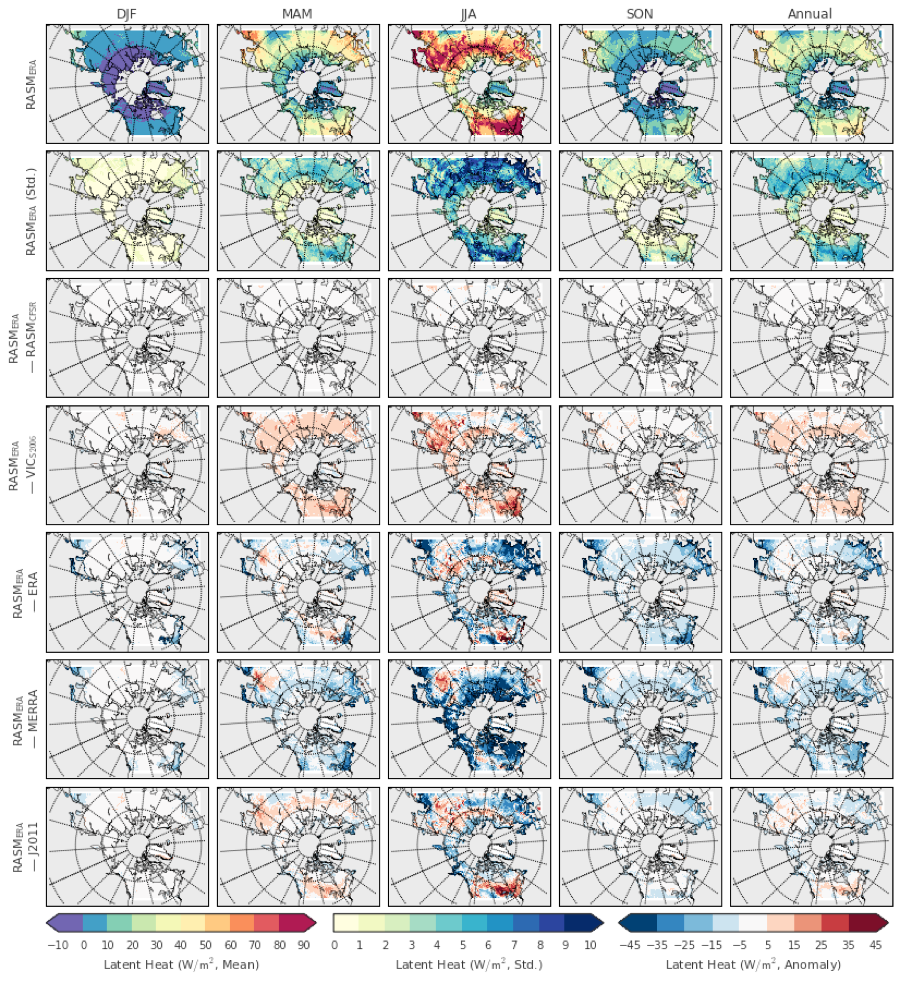
\includegraphics[width=12cm,keepaspectratio]{ch3_S5}
    \caption{Seasonal and annual average latent heat flux (LE).
    Time period: Sep. 1989 – Aug. 2014.}
\end{figure}

\begin{figure}
    \centering
    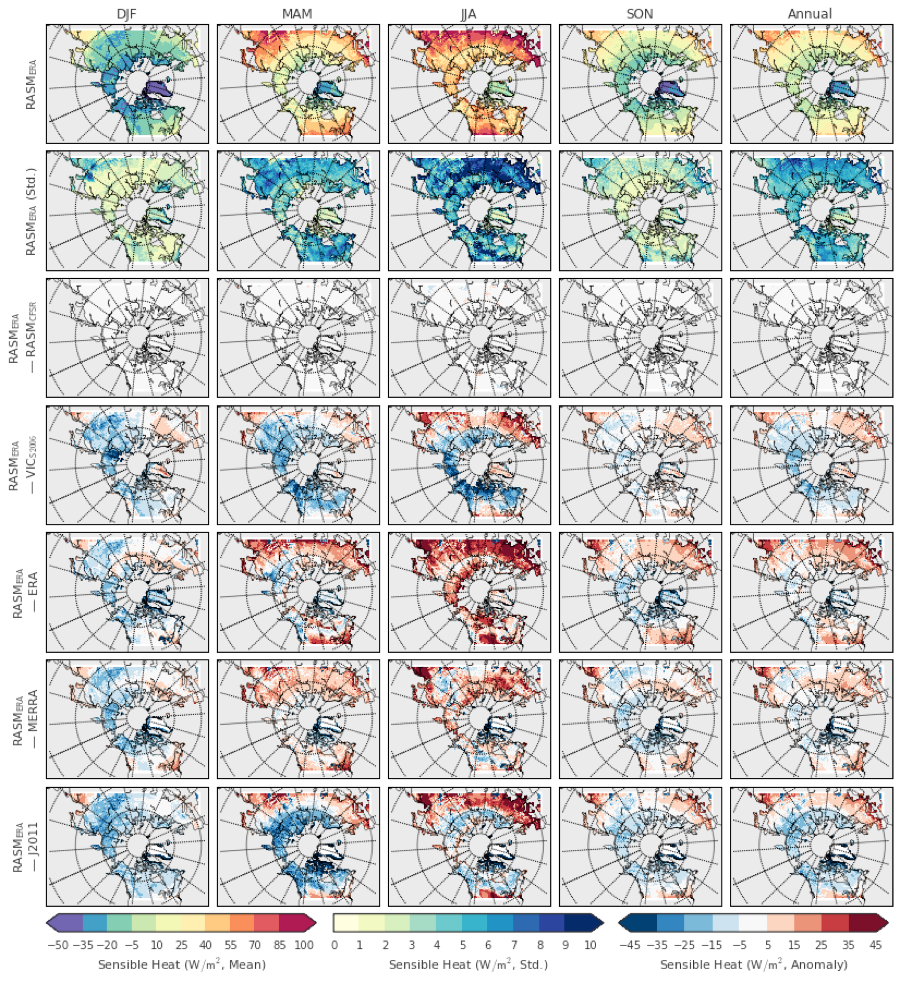
\includegraphics[width=12cm,keepaspectratio]{ch3_S6}
    \caption{Seasonal and annual average sensible heat flux (H).
    Time period: Sep. 1989 – Aug. 2014.}
\end{figure}

\begin{figure}
    \centering
    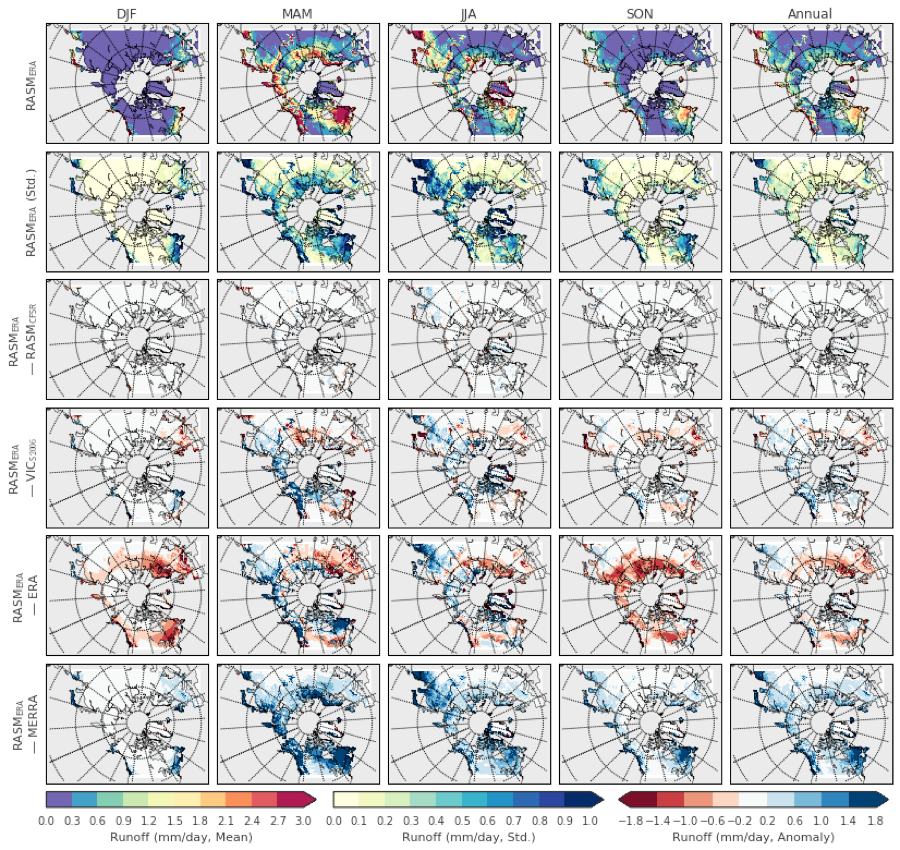
\includegraphics[width=12cm,keepaspectratio]{ch3_S7}
    \caption{Seasonal and annual runoff (Q).
    Time period: Sep. 1989 – Aug. 2014.}
\end{figure}

\begin{figure}
    \centering
    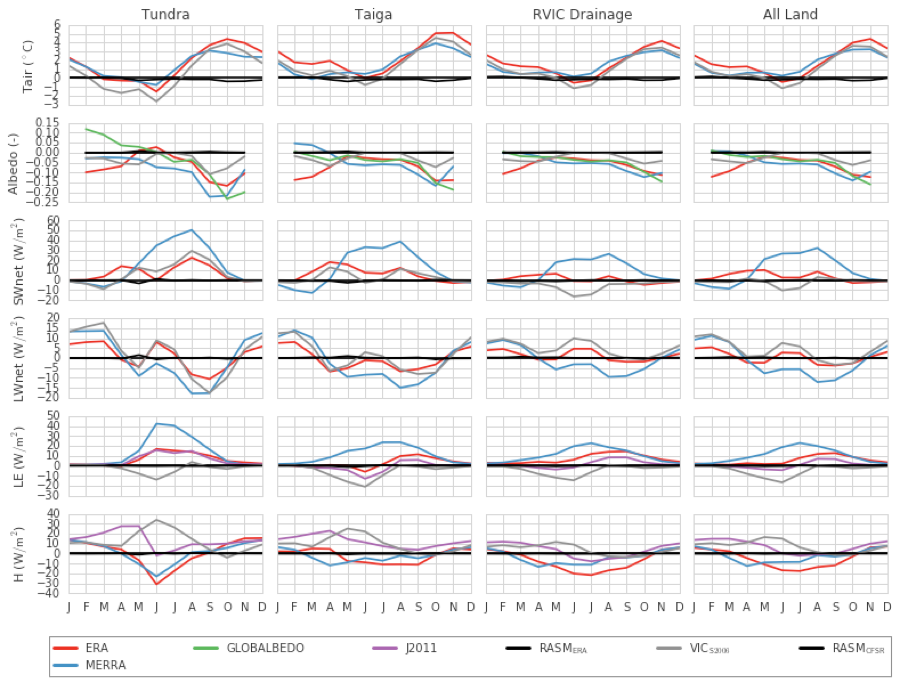
\includegraphics[width=12cm,keepaspectratio]{ch3_S8}
    \caption{Difference (RASM – X) in average seasonal cycles of surface air temperature (Tair), albedo, net shortwave radiation (SWnet), net longwave radiation (LWnet), latent heat flux (LE), and sensible heat flux (H) for tundra, taiga, RVIC drainage, and full model domain.
    Time period: 1990-2014.}
\end{figure}

\begin{figure}
    \centering
    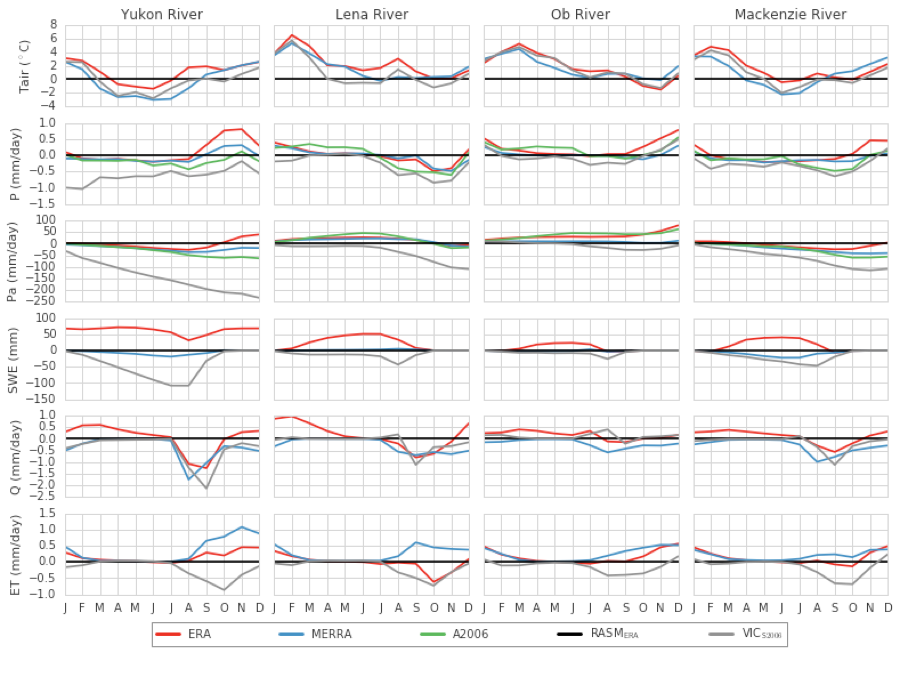
\includegraphics[width=12cm,keepaspectratio]{ch3_S9}
    \caption{Difference (RASM – X) in average seasonal cycles of surface air temperature (Tair), precipitation (P), accumulated precipitation (Pa), runoff (Q), evapotranspiration (ET) and snow water equivalent (SWQ) for four of the largest river basins in the RASM domain.
    Time period: 1990-2014.}
\end{figure}

\section{Tables}

\begin{table}[]
\centering
\caption{Summary of land surface parameters used by the VIC model.}
\label{table:s1}
\resizebox{\textwidth}{!}{
\begin{tabular}{ll}
\hline
\textbf{Parameters}                                                        & \textbf{Values or Source}           \\ \hline
Physical parameters (soil density, saturated hydraulic conductivity, etc.) & \citet{Sheffield_2006}              \\
Calibratable parameters (baseflow, infiltration, etc.)                     & \citet{Sheffield_2006},             \\
                                                                           & Inside Permafrost Region: Dsmax ≈ 0 \\
Soil depths                                                                & 0.1 m / 0.9 m / 2.5 m               \\
Vegetation resistance parameters                                           & \citet{Nijssen_1997}                \\
Canopy Layers                                                              & 1                                   \\
Land Surface Emissivity                                                    & 0.97                                \\
Bare Surface Albedo                                                        & 0.55                                \\
Fresh Snow Albedo                                                          & 0.85                                \\
Maximum Snow Covered Vegetation Albedo                                     & \citet{Barlage_2005}                \\ \hline
\end{tabular}
}
\end{table}

\begin{table}[]
\centering
\caption{Summary of land-atmosphere coupled variables in RASM.}
\label{table:s2}
 \resizebox{\textwidth}{!}{
\begin{tabular}{ll}
\hline
Coupled Fields – Coupler to Land (units)                   & Coupled Fields – Land to Coupler (units)            \\ \hline
Height of atmosphere lowest model level (m)                & Liquid runoff flux (kg m-1 s-1)                     \\
Zonal wind at atmosphere lowest model level (m/s)          & Surface temperature (K)                             \\
Meridional wind at atmosphere lowest model level (m/s)     & 2-m reference air temperature (K)                   \\
Potential temperate at atmosphere lowest model level (K)   & 2-m reference specific humidity (-)                 \\
Specific humidity at atmosphere lowest model level (-)     & Direct, visible surface albedo (-)                  \\
Atmospheric pressure at atmosphere lowest model level (Pa) & Direct, near-infrared surface albedo (-)            \\
Temperature at atmosphere lowest model level (K)           & Diffuse, visible surface albedo (-)                 \\
Downwelling longwave radiation flux (W m-2)                & Diffuse, near-infrared surface albedo (-)           \\
Direct near-infrared shortwave radiation flux (W m-2)      & Snow height (m)                                     \\
Direct visible shortwave radiation flux (W m-2)            & Log Z0 (-)                                          \\
Diffuse near-infrared shortwave radiation flux (W m-2)     & Zonal wind stress (Pa)                              \\
Diffuse visible shortwave radiation flux (W m-2)           & Meridional wind stress (Pa)                         \\
Convective liquid precipitation flux (kg m-1 s-1)          & Latent heat flux (W m-2)                            \\
Large scale liquid precipitation flux (kg m-1 s-1)         & Sensible heat flux (W m-2)                          \\
Convective frozen precipitation flux (kg m-1 s-1)          & Upwelling longwave radiation flux (W m-2)           \\
Large scale frozen precipitation flux (kg m-1 s-1)         & Evaporation flux (kg m-1 s-1)                       \\
                                                           & Net shortwave radiation flux at the surface (W m-2) \\ \hline
\end{tabular}
}
\end{table}

\begin{table}[]
\centering
\caption{Summary of comparison datasets used to compare to RASM land surface output.}
\label{table:s3}
\resizebox{\textwidth}{!}{
\begin{tabular}{llllll}
\hline
\textbf{Dataset}                                                                 & \textbf{Label} & \textbf{Data Type}              & \textbf{Spatial Coverage}        & \textbf{Temporal Coverage} & \textbf{Reference}           \\ \hline
ECMWF’s ERA-interim Reanalysis                                                   & ERA            & Reanalysis                      & Global - T255 (approx. 80 km)    & 1979-present               & \citet{Dee_2011}             \\
                                                                                 &                &                                 &                                  & 3-hourly                   &                              \\
NASA’s Modern-Era Retrospective Analysis for Research and Applications           & MERRA          & Reanalysis                      & Global – 1/2$^{\circ}$ × 2/3 $^{\circ}$            & 1979-present               & \citet{Rienecker_2011}       \\
                                                                                 &                &                                 &                                  & 3-hourly                   &                              \\
Global Meteorological Forcing Dataset for land surface modeling                  & S2006          & Bias Corrected Reanalysis       & Global - 1$^{\circ}$                      & 1948-2010, 3-hourly        & \citet{Sheffield_2006}       \\
Global 1/2$^{\circ}$ Gridded Meteorological VIC Forcing Data Set                          & A2006          & Bias Corrected Reanalysis       & Global Land – 0.5$^{\circ}$               & 1948-2007, daily           & \citet{Adam_2006}            \\
Northern Hemisphere EASE-Grid 2.0 Weekly Snow Cover Extent, Version 4            & NSIDC          & Remote Sensing                  & Northern Hemisphere Land - 25 km & 1966-2014, weekly          & \citet{Brodzik_2013}         \\
ESA High Resolution Global Albedo Data Set                                       & GlobAlbedo     & Remote Sensing                  & Global Land – 1km                & 1998-2011, monthly         & \citet{Muller_2012}          \\
Empirically Upscaled Gridded FLUXNET Data Set                                    & J2011          & Reanalysis / Observations       & Global Land – 0.5$^{\circ}$               & 1982-2011                  & \citet{Jung_2011}            \\
Regional, Electronic, Hydrographic Data Network For the Arctic Region, Version 4 & R-ArcticNET    & In-situ Streamflow Observations & Pan-arctic, 3754 gauges          & 1960-2001,                 & \citet{Lammers_2001}         \\
                                                                                 &                &                                 &                                  & monthly                    &                              \\
AmeriFlux: Regional flux tower network database                                  & AmeriFlux      & In-situ Flux Tower Observations & Global, 2 stations used          & 1994-1995 (used)           &                              \\ \hline
\end{tabular}
}
\end{table}

\begin{table}[]
\centering
\caption{Variables analyzed and datasets each variable is compared to.}
\label{table:s4}
\resizebox{\textwidth}{!}{

\begin{tabular}{lll}
\hline
\textbf{Variable}     & \textbf{Abbreviation} & \textbf{Compared to:}        \\ \hline
2m Air Temperature    & Tair                  & ERA, MERRA, S2006, AmeriFlux \\
Surface Albedo        & Albedo                & ERA, MERRA, GlobAlbedo       \\
Shortwave Radiation   & SW\{in,up,net\}       & ERA, MERRA, S2006            \\
Longwave Radiation    & LW\{in,up,net\}       & ERA, MERRA, S2006            \\
Latent Heat           & LH                    & ERA, MERRA, J2011, AmeriFlux \\
Sensible Heat         & H                     & ERA, MERRA, J2011, AmeriFlux \\
Total Precipitation   & P                     & ERA, MERRA, S2006, A2006     \\
Total Runoff          & Q                     & ERA, MERRA, R-ArcticNET      \\
Evapotranspiration    & ET                    & ERA, MERRA                   \\
Snow Water Equivalent & SWQ                   & ERA, MERRA                   \\
Snow Cover Extent     & SCE                   & ERA, MERRA, NSIDC            \\ \hline
\end{tabular}
}
\end{table}

\begin{table}[]
\centering
\caption{Seasonal and annual averages for selected variables for the tundra and taiga bioregions. Time period 1990-2014.}
\label{table:s5}
\resizebox{\textwidth}{!}{

\begin{tabular}{lllllllllll}
Taiga                                          &                              &        &        &        & Tundra &        &        &        &        &        \\
                                               & DJF                          & MAM    & JJA    & SON    & Annual & DJF    & MAM    & JJA    & SON    & Annual \\
Albedo (-)                                     &                              &        &        &        &        &        &        &        &        &        \\
ERA                                            & 0.3                          & 0.26   & 0.15   & 0.19   & 0.2    & 0.53   & 0.54   & 0.29   & 0.33   & 0.4    \\
MERRA                                          & 0.47                         & 0.3    & 0.12   & 0.16   & 0.2    & 0.55   & 0.51   & 0.2    & 0.27   & 0.33   \\
RASMCFSR                                       & 0.44                         & 0.32   & 0.18   & 0.3    & 0.27   & 0.62   & 0.57   & 0.31   & 0.54   & 0.45   \\
RASMERA                                        & 0.44                         & 0.32   & 0.18   & 0.3    & 0.26   & 0.62   & 0.57   & 0.3    & 0.54   & 0.44   \\
Bowen Ratio, B (-)                             &                              &        &        &        &        &        &        &        &        &        \\
2.82                                           & 1.2                          & 0.52   & -0.22  & 0.42   & 2.98   & 1.52   & 0.28   & -1.57  & -0.17  & 2.82   \\
-48.06                                         & 0.6                          & 0.51   & -0.06  & 0.37   & 54.5   & 0.46   & 0.67   & -1.33  & 0.36   & -48.06 \\
-9                                             & 1.14                         & 0.76   & -1     & 0.53   & 108.32 & -0.08  & 1.44   & 14.62  & -1.59  & -9     \\
14.27                                          & 1.13                         & 0.76   & -0.44  & 0.54   & 18.6   & -1.15  & 1.55   & 1.81   & -0.94  & 14.27  \\
Evapotranspiration, ET (mm/day)                &                              &        &        &        &        &        &        &        &        &        \\
ERA                                            & 0.06                         & 0.82   & 2.35   & 0.59   & 0.95   & 0.07   & 0.33   & 1.33   & 0.3    & 0.51   \\
MERRA                                          & 0.08                         & 1.14   & 3.09   & 0.69   & 1.25   & 0      & 0.48   & 2.15   & 0.27   & 0.72   \\
RASMCFSR                                       & 0.01                         & 0.82   & 2.32   & 0.32   & 0.86   & -0.02  & 0.29   & 1.01   & 0.08   & 0.34   \\
RASMERA                                        & 0.01                         & 0.84   & 2.32   & 0.32   & 0.88   & -0.02  & 0.29   & 1.02   & 0.08   & 0.35   \\
Latent Heat Flux, LE (W/m2)                    &                              &        &        &        &        &        &        &        &        &        \\
ERA                                            & 2.08                         & 24.72  & 67.81  & 17.41  & 27.95  & 2.01   & 10.42  & 38.49  & 8.81   & 14.9   \\
MERRA                                          & 2.46                         & 33.94  & 87.85  & 19.74  & 35.92  & 0.05   & 14.86  & 61.26  & 7.82   & 20.92  \\
RASMCFSR                                       & 0.44                         & 24.41  & 66.11  & 9.31   & 24.95  & -0.76  & 9.04   & 29.07  & 2.27   & 9.85   \\
RASMERA                                        & 0.47                         & 24.91  & 66.13  & 9.41   & 25.41  & -0.76  & 9.1    & 29.3   & 2.37   & 10.08  \\
Net Longwave Radiation Flux, LWnet (W/m2)      &                              &        &        &        &        &        &        &        &        &        \\
ERA                                            & -32.74                       & -56.8  & -58.39 & -40.51 & -47.07 & -31.08 & -43.81 & -45.65 & -35.25 & -38.92 \\
MERRA                                          & -28.91                       & -54.3  & -65.93 & -44.15 & -48.32 & -21.81 & -42.68 & -60.67 & -33.28 & -39.59 \\
RASMCFSR                                       & -39.52                       & -53.29 & -55.62 & -38.71 & -46.72 & -38.18 & -47.65 & -48.93 & -33.59 & -42.01 \\
RASMERA                                        & -39.57                       & -53.89 & -55.72 & -38.55 & -46.99 & -38.21 & -48.03 & -48.86 & -33.45 & -42.18 \\
P-E (mm/day)                                   &                              &        &        &        &        &        &        &        &        &        \\
ERA                                            & 0.9                          & 0.49   & 0.26   & 1.25   & 0.73   & 0.73   & 0.58   & 0.52   & 1.13   & 0.74   \\
MERRA                                          & 0.86                         & 0.18   & -0.73  & 1.06   & 0.35   & 0.77   & 0.43   & -0.39  & 1.1    & 0.48   \\
RASMCFSR                                       & 0.97                         & 0.62   & 0.04   & 1.31   & 0.74   & 0.84   & 0.74   & 0.7    & 1.33   & 0.91   \\
RASMERA                                        & 0.96                         & 0.6    & 0.07   & 1.32   & 0.73   & 0.83   & 0.73   & 0.73   & 1.36   & 0.91   \\
Precipitation, P (mm/day)                      &                              &        &        &        &        &        &        &        &        &        \\
ERA                                            & 0.96                         & 1.31   & 2.61   & 1.85   & 1.68   & 0.8    & 0.91   & 1.85   & 1.43   & 1.25   \\
MERRA                                          & 0.94                         & 1.33   & 2.36   & 1.74   & 1.59   & 0.83   & 0.94   & 1.8    & 1.42   & 1.25   \\
RASMCFSR                                       & 0.98                         & 1.44   & 2.36   & 1.63   & 1.6    & 0.82   & 1.02   & 1.72   & 1.41   & 1.24   \\
RASMERA                                        & 0.97                         & 1.44   & 2.39   & 1.64   & 1.61   & 0.81   & 1.02   & 1.75   & 1.44   & 1.26   \\
Total Runoff, Q (mm/day)                       &                              &        &        &        &        &        &        &        &        &        \\
ERA                                            & 0.55                         & 1.18   & 0.92   & 1.07   & 0.93   & 0.21   & 0.87   & 1.38   & 0.9    & 0.84   \\
MERRA                                          & 0.1                          & 0.76   & 0.31   & 0.18   & 0.34   & 0.09   & 0.72   & 0.83   & 0.22   & 0.46   \\
RASMCFSR                                       & 0.13                         & 1.51   & 0.8    & 0.47   & 0.72   & 0.09   & 1.49   & 1.55   & 0.43   & 0.89   \\
RASMERA                                        & 0.13                         & 1.51   & 0.8    & 0.47   & 0.73   & 0.09   & 1.52   & 1.54   & 0.45   & 0.91   \\
Runoff Ratio, Q/P (-)                          &                              &        &        &        &        &        &        &        &        &        \\
ERA                                            & 0.52                         & 0.93   & 0.33   & 0.58   & 0.53   & 0.18   & 0.95   & 0.88   & 0.62   & 0.68   \\
MERRA                                          & 0.06                         & 0.49   & 0.11   & 0.07   & 0.17   & 0.04   & 0.59   & 0.42   & 0.1    & 0.29   \\
RASMCFSR                                       & 0.06                         & 0.98   & 0.31   & 0.22   & 0.4    & 0.03   & 1.38   & 0.93   & 0.23   & 0.69   \\
RASMERA                                        & 0.07                         & 0.98   & 0.31   & 0.22   & 0.4    & 0.03   & 1.42   & 0.91   & 0.23   & 0.7    \\
                                               & Sensible Heat Flux, H (W/m2) &        &        &        &        &        &        &        &        &        \\
ERA                                            & -13.76                       & 29.02  & 34.23  & -2.46  & 11.67  & -10.3  & 5.79   & 21.67  & -1.26  & 3.95   \\
MERRA                                          & -11.78                       & 20.58  & 40.64  & -1.28  & 11.97  & -12.27 & 7.06   & 36.81  & -4.92  & 6.61   \\
RASMCFSR                                       & -17.72                       & 28.49  & 45.2   & -0.82  & 13.68  & -29.25 & 2.65   & 41.17  & -15.93 & -0.45  \\
RASMERA                                        & -17.5                        & 28.76  & 45.39  & -0.84  & 14.16  & -29.2  & 2.92   & 41.05  & -15.93 & -0.09  \\
Downward Shortwave Radiation Flux, SWin (W/m2) &                              &        &        &        &        &        &        &        &        &        \\
ERA                                            & 25.37                        & 175.49 & 209.65 & 57.52  & 116.63 & 8.99   & 159.39 & 198.4  & 34.99  & 100.02 \\
MERRA                                          & 26.22                        & 172.98 & 231.39 & 67.5   & 124.22 & 8.89   & 150.52 & 214.45 & 40.59  & 103.25 \\
RASMCFSR                                       & 33.22                        & 169.3  & 206.52 & 65.92  & 118.34 & 11.57  & 158.58 & 186.52 & 39.69  & 98.62  \\
RASMERA                                        & 33.63                        & 170.28 & 206.83 & 65.7   & 119.72 & 11.71  & 159.17 & 185.69 & 39.36  & 99.62  \\
Net Shortwave Radiation Flux, SWnet (W/m2)     &                              &        &        &        &        &        &        &        &        &        \\
ERA                                            & 18.05                        & 129.79 & 178.98 & 46.96  & 93.15  & 4.73   & 74.21  & 138.21 & 24.08  & 60.08  \\
MERRA                                          & 14.13                        & 121.24 & 204.8  & 56.8   & 99.03  & 3.92   & 71.68  & 174.74 & 30.3   & 69.94  \\
RASMCFSR                                       & 19.12                        & 114.79 & 169.92 & 46.63  & 87.31  & 4.74   & 67.21  & 128.81 & 19.1   & 54.68  \\
RASMERA                                        & 19.38                        & 116.15 & 170.2  & 46.59  & 88.57  & 4.8    & 68.12  & 128.74 & 19.14  & 55.57  \\
Upward Shortwave Radiation Flux, SWup (W/m2)   &                              &        &        &        &        &        &        &        &        &        \\
ERA                                            & 7.32                         & 45.7   & 30.67  & 10.56  & 23.48  & 4.26   & 85.18  & 60.19  & 10.92  & 39.94  \\
MERRA                                          & 11.71                        & 50.68  & 26.62  & 10.64  & 24.82  & 4.79   & 75.79  & 44.91  & 10.25  & 33.79  \\
RASMCFSR                                       & 14.11                        & 54.5   & 36.61  & 19.29  & 31.03  & 6.83   & 91.37  & 57.7   & 20.59  & 43.94  \\
RASMERA                                        & 14.25                        & 54.13  & 36.63  & 19.1   & 31.15  & 6.91   & 91.05  & 56.95  & 20.22  & 44.05  \\
Surface Air Temperature, Tair (C)              &                              &        &        &        &        &        &        &        &        &        \\
ERA                                            & -20.36                       & -2.88  & 14.07  & -2.36  & -2.86  & -25.58 & -12.62 & 7.6    & -8.17  & -9.66  \\
MERRA                                          & -21.59                       & -4     & 14.55  & -3.36  & -3.58  & -24.8  & -11.2  & 8.36   & -8.76  & -9.08  \\
RASMCFSR                                       & -23.28                       & -4.46  & 13.12  & -7.15  & -5.44  & -28.49 & -12.08 & 7.21   & -12.84 & -11.54 \\
RASMERA                                        & -23.39                       & -4.28  & 13.3   & -6.9   & -5.21  & -28.39 & -11.9  & 7.38   & -12.45 & -11.24
\end{tabular}
}
\end{table}

\appendix
\raggedbottom\sloppy

\chapter{Scientific Software Development}
\label{chap:software}

\section{Introduction}
In conjunction with the preparation of this dissertation, I have had the opportunity to contribute to a range of open source software projects.
In this section, I briefly introduce the main projects that I have contributed to and that contributed to this dissertation.
Some of these tools were developed specifically for the scientific research included in this chapter (e.g. RASM and RVIC) while others were tools used for processing and analysis of scientific data (e.g. xarray).
VIC version 5.0.0 was a major development project, developed to provide additional infrastructure to the VIC model and enabling a new scientific applications in RASM and other VIC applications.

Nearly all of the software I have written and used during my time working on this dissertation is publicly available and open-source.
With the exception of the RASM model source code, the other packages described in this section were developed entirely in the open.
Transparent scientific software development facilitates reuse and extension and review by the broader scientific community

\section{VIC Version 5}
\label{sec:vic_dev}
The Variable Infiltration Capacity (VIC) model is a macro-scale semi-distributed hydrologic model.
VIC development began in the early 1990s and it has been used extensively, applied from basin to global scales.
VIC has been applied in a many use cases, including the construction of hydrologic data sets, trend analysis, data evaluation and assimilation, forecasting, coupled climate modeling, and climate change impact analysis.
Ongoing operational applications of the VIC model include the University of Washington's drought monitor and forecast systems, and NASA's land data assimilation systems.
The development of VIC version 5 focused on reconfiguring the legacy VIC source code to support a wider range of modern modeling applications.
The VIC source code has been moved to a public Github repository to encourage participation by the broader user and developer.
The reconfiguration has separated the physical core of the model from the driver, which is responsible for memory allocation, pre- and post-processing and I/O.
VIC 5 includes four drivers that use the same physical model core: classic, image, CESM, and Python.
The classic driver supports legacy VIC configurations and runs in the traditional time-before-space configuration.
The image driver includes a space-before-time configuration, NetCDF I/O, and uses MPI for parallel processing.
This configuration will facilitate the direct coupling of streamflow routing, reservoir, and irrigation processes within VIC.
The image driver is the foundation of the CESM driver; which couples VIC to CESM's CPL7 and a prognostic atmosphere.
The Python driver provides interactive access to the functions and datatypes of VIC's physical core from a Python interface.
Finally, VIC 5.0 is distributed with a robust test infrastructure, components of which routinely run during development using the Travis CI continuous integration service.

\section{RASM}
\label{sec:rasm_dev}

The RASM model has been described in detail in Chapters \ref{chap:rasm}, \ref{chap:land_surface}, \ref{chap:streamflow}.
The source code that makes up RASM is scheduled to be released upon publication of Maslowski et al (Manuscript in preparation).

% Brunke_2016

\section{RVIC}
\label{sec:rvic_dev}

RVIC is a source-to-sink linear routing model used to route streamflows from runoff produced in macro-scale hydrologic models such as VIC.
RVIC is written in a combination Python and C and is publicly available in \citet{Hamman_2015}
RVIC's convolution routine included in RASM has been written in Fortran and will be distributed with the rest of the RASM source code.

\section{xarray}
\label{sec:xarray_dev}

\textbf{xarray} is an community built, open source project, and Python package that provides a toolkit and data structures for N-dimensional labeled arrays \citep{Hoyer_2016}.
I have been contributing to the \textbf{xarray} project since May 2014 and the package has been a core tool in this dissertation.
\textbf{xarray} includes an API inspired by pandas \citep{mckinney_2010} and the Common Data Model for self-described scientific data \citep{Rew_1990,Brown_1993}.
Key features of the \textbf{xarray} package include label-based indexing and arithmetic, interoperability with the core scientific Python packages (e.g., pandas, NumPy \citep{Jones_2001}, Matplotlib \citep{van_der_Walt_2011}), out-of-core computation on datasets that don't fit into memory, a wide range of serialization and input/output options (e.g. netCDF, HDF, GRIB1/2), and advanced multi-dimensional data manipulation tools such as group-by and resampling.
It has been widely adopted in the geoscience community \citep[e.g.][]{xgcm,Dawson_2016a,Dawson_2016b}, but has also been used in physics \citep[e.g.][]{pycalphad}, time series analytics \citep{cesium}, and finance.
On
\textbf{xarray} is licensed as an open
source package using the Apache, v2.0 license.
A complete description of \textbf{xarray} is available in \citet{Hoyer_2016} and in the \textbf{xarray} documentation \citep{xarray_docs}.


\vita{Joseph (Joe) J. Hamman was born on July 31, 1984 in Phoenix Arizona.
He Graduated from Prescott High School, Prescott Arizona in May of 2003.
Joe earned a Bachelor of Science in Civil Engineering from the Department of Civil and Environmental Engineering at the University of Arizona in May of 2007.
He earned a Master of Science in Civil Engineering from the Department of Civil and Environmental Engineering at the University of Washington in June of 2012.
Joe defended this dissertation on October 3, 2016 at the University of Washington.
}

\end{document}
